\documentclass[12pt,oneside]{report}
% ===================== Codificacion e idioma =====================
\usepackage[utf8]{inputenc}
\usepackage[T1]{fontenc}
\usepackage[spanish,es-noquoting,es-nolists,es-noshorthands]{babel}
\usepackage{lmodern}
\usepackage{microtype}

% ===================== Matematicas =====================
\usepackage{amsmath,amssymb,amsthm,mathtools}
\usepackage{bm}

% ===================== Formato =====================
\usepackage[letterpaper,margin=2.6cm,bottom=3cm,headheight=16pt]{geometry}
\usepackage{setspace}
\usepackage{graphicx}
\usepackage{booktabs}
\usepackage{longtable}
\usepackage{array}
\usepackage{multirow}
\usepackage{float}
\usepackage[font=small,labelfont=bf,width=.92\textwidth]{caption}
\usepackage{subcaption}
\usepackage{enumitem}
\usepackage{xcolor}
\usepackage{fancyhdr}
\usepackage[ruled,vlined,linesnumbered,spanish]{algorithm2e}
\usepackage{tikz}
\usetikzlibrary{arrows.meta,positioning,calc,decorations.pathreplacing,shapes.geometric}
\usepackage[round,authoryear]{natbib}
\usepackage{xurl}
\usepackage[hidelinks,breaklinks]{hyperref}
\usepackage[nameinlink,spanish]{cleveref}


% ===================== Listados de codigo fuente =====================
\usepackage{listings}

% listings no maneja UTF-8 por si mismo con pdflatex: hay que declarar
% explicitamente cada caracter acentuado. Sin esto, los comentarios en
% espanol del codigo fuente salen truncados o con caracteres perdidos.
\lstset{
  inputencoding=utf8,
  extendedchars=true,
  literate=%
    {á}{{\'a}}1 {é}{{\'e}}1 {í}{{\'i}}1 {ó}{{\'o}}1 {ú}{{\'u}}1
    {Á}{{\'A}}1 {É}{{\'E}}1 {Í}{{\'I}}1 {Ó}{{\'O}}1 {Ú}{{\'U}}1
    {ñ}{{\~n}}1 {Ñ}{{\~N}}1 {ü}{{\"u}}1 {Ü}{{\"U}}1
    {¿}{{?`}}1 {¡}{{!`}}1 {°}{{\textdegree}}1 {º}{{\textordmasculine}}1
    {–}{{--}}1 {—}{{---}}1 {“}{{``}}1 {”}{{''}}1 {‘}{{`}}1 {’}{{'}}1
    {…}{{\ldots}}1 {≤}{{$\leq$}}1 {≥}{{$\geq$}}1 {×}{{$\times$}}1
    {Δ}{{$\Delta$}}1 {∂}{{$\partial$}}1 {α}{{$\alpha$}}1 {λ}{{$\lambda$}}1
    {μ}{{$\mu$}}1 {φ}{{$\varphi$}}1 {ρ}{{$\rho$}}1 {σ}{{$\sigma$}}1
    {τ}{{$\tau$}}1 {θ}{{$\theta$}}1 {γ}{{$\gamma$}}1 {δ}{{$\delta$}}1
    {ε}{{$\varepsilon$}}1 {∞}{{$\infty$}}1 {≠}{{$\neq$}}1 {→}{{$\to$}}1
    {∈}{{$\in$}}1 {·}{{\textperiodcentered}}1
}

\definecolor{codfondo}{HTML}{FAFAFA}
\definecolor{codcomentario}{HTML}{5E7A87}
\definecolor{codclave}{HTML}{0057A3}
\definecolor{codcadena}{HTML}{9B5000}
\definecolor{codnumero}{HTML}{9AA5AD}
\definecolor{codmarco}{HTML}{DEE3E6}

\lstdefinestyle{python}{
  language=Python,
  basicstyle=\ttfamily\scriptsize,
  keywordstyle=\color{codclave}\bfseries,
  commentstyle=\color{codcomentario}\itshape,
  stringstyle=\color{codcadena},
  numberstyle=\ttfamily\tiny\color{codnumero},
  numbers=left, numbersep=7pt,
  backgroundcolor=\color{codfondo},
  frame=single, framerule=.4pt, rulecolor=\color{codmarco},
  breaklines=true, breakatwhitespace=false,
  postbreak=\mbox{\textcolor{codnumero}{$\hookrightarrow$}\space},
  showstringspaces=false,
  tabsize=4,
  captionpos=b,
  xleftmargin=1.6em, xrightmargin=.2em,
  aboveskip=1.1em, belowskip=1.1em,
  morekeywords={self,True,False,None,dataclass,field,replace},
}
\lstset{style=python}
\renewcommand{\lstlistingname}{Listado}
\renewcommand{\lstlistlistingname}{Índice de listados}

% ===================== Colores =====================
\definecolor{azultesis}{HTML}{0072B2}
\definecolor{naranja}{HTML}{E69F00}
\definecolor{verdetesis}{HTML}{009E73}
\definecolor{rojotesis}{HTML}{D55E00}
\definecolor{grisclaro}{HTML}{F2F2F2}
\definecolor{grismedio}{HTML}{7F7F7F}

\hypersetup{colorlinks=true, linkcolor=azultesis, citecolor=verdetesis,
            urlcolor=azultesis, linktoc=all}

% ===================== Encabezados =====================
\pagestyle{fancy}
\fancyhf{}
\renewcommand{\headrulewidth}{0.3pt}
\fancyhead[L]{\small\nouppercase{\leftmark}}
\fancyhead[R]{\small\thepage}
\fancypagestyle{plain}{\fancyhf{}\renewcommand{\headrulewidth}{0pt}\fancyfoot[C]{\small\thepage}}

% ===================== Entornos de teorema =====================
\theoremstyle{plain}
\newtheorem{theorem}{Teorema}[chapter]
\newtheorem{proposition}[theorem]{Proposición}
\newtheorem{lemma}[theorem]{Lema}
\newtheorem{corollary}[theorem]{Corolario}
\theoremstyle{definition}
\newtheorem{definition}[theorem]{Definición}
\newtheorem{example}[theorem]{Ejemplo}
\newtheorem{assumption}[theorem]{Hipótesis}
\theoremstyle{remark}
\newtheorem{remark}[theorem]{Observación}
\newtheorem{criticism}[theorem]{Discusión crítica}
\crefname{criticism}{discusión crítica}{discusiones críticas}
\Crefname{criticism}{Discusión crítica}{Discusiones críticas}
\crefname{remark}{observación}{observaciones}
\Crefname{remark}{Observación}{Observaciones}
% Ecuaciones: solo el número entre paréntesis, p. ej. «de (3.11)».
\crefformat{equation}{(#2#1#3)}
\Crefformat{equation}{(#2#1#3)}
\crefrangeformat{equation}{(#3#1#4) a~(#5#2#6)}
\crefmultiformat{equation}{(#2#1#3)}{ y~(#2#1#3)}{, (#2#1#3)}{ y~(#2#1#3)}
\Crefmultiformat{equation}{(#2#1#3)}{ y~(#2#1#3)}{, (#2#1#3)}{ y~(#2#1#3)}

% Caja para los resultados originales del trabajo
\usepackage[most]{tcolorbox}
\newtcolorbox{aporte}[1][]{
  colback=grisclaro, colframe=azultesis, boxrule=.6pt, arc=1.6pt,
  left=6pt,right=6pt,top=5pt,bottom=5pt, #1}

% ===================== Notacion =====================
\newcommand{\R}{\mathbb{R}}
\newcommand{\N}{\mathbb{N}}
\newcommand{\Prob}{\mathbb{P}}
\newcommand{\Esp}{\mathbb{E}}
\newcommand{\ind}{\mathbf{1}}
\newcommand{\dB}{\partial_B}
\newcommand{\dC}{\partial}
\newcommand{\KA}{\mathit{KA}}
\newcommand{\VP}{\mathit{VP}}
\newcommand{\CONAB}{\mathit{CONAB}}
\newcommand{\SMLV}{\mathit{SMLV}}
\newcommand{\AUF}{\mathit{AUF}}
\newcommand{\RAB}{\mathit{RAB}}
\newcommand{\CAI}{\mathit{CAI}}
\newcommand{\DURA}{\mathit{DURA}}
\newcommand{\npx}[2]{{}_{#1}p_{#2}}
\newcommand{\nqx}[2]{{}_{#1}q_{#2}}
\newcommand{\med}{\operatorname{med}}
\newcommand{\sgn}{\operatorname{sgn}}
\newcommand{\dom}{\operatorname{dom}}
\newcommand{\Lip}{\operatorname{Lip}}
\DeclareMathOperator*{\argmin}{arg\,min}

% Espaciado de tablas
\renewcommand{\arraystretch}{1.15}
\setlength{\tabcolsep}{5pt}

% Titulos de capitulo compactos
\usepackage{titlesec}
\titleformat{\chapter}[display]
  {\normalfont\huge\bfseries\color{azultesis}}
  {\chaptertitlename\ \thechapter}{14pt}{\Huge}
\titlespacing*{\chapter}{0pt}{-18pt}{28pt}

% Enlace al repositorio de la tesis (codigo, tablas completas y aplicacion).
\newcommand{\repositorio}{\url{https://github.com/elagosd/tesis-rentas-vitalicias}}

% Generado automaticamente por py/generar_macros_tex.py -- NO editar a mano.
\newcommand{\datoSMLV}{1\,750\,905}
\newcommand{\datoKAmin}{440\,140\,099}
\newcommand{\datoKAminMill}{440}
\newcommand{\datoPendienteAfin}{245{,}1050}
\newcommand{\datoPendienteAUF}{245{,}5588}
\newcommand{\datoSaltoAUF}{0{,}4538}
\newcommand{\datoCondicionamientoDirecto}{245{,}1}
\newcommand{\datoCondicionamientoInverso}{4079{,}9}
\newcommand{\datoNMeses}{1439}
\newcommand{\datoVigenciaCorte}{1321}
\newcommand{\datoAniosProyeccion}{119{,}9}
\newcommand{\datoAniosVigencia}{110{,}1}
\newcommand{\datoRhoQuiebre}{1{,}001262}
\newcommand{\datoRhoQuiebrePct}{0{,}1262}
\newcommand{\datoAnchoRacimo}{1{,}1488}
\newcommand{\datoNumQuiebres}{333}
\newcommand{\datoIPCuno}{6{,}34}
\newcommand{\datoIPCdos}{4{,}77}
\newcommand{\datoIPClp}{3{,}00}
\newcommand{\datoDeslizamiento}{0{,}13}
\newcommand{\datoGastosReserva}{5{,}0}
\newcommand{\datoCambioGrupo}{0{,}6}
\newcommand{\datoInteresRP}{4{,}20}
\newcommand{\datoGastosRP}{1{,}5}
\newcommand{\datoDeslizRPalto}{4{,}23}
\newcommand{\datoDeslizRPbajo}{2{,}53}
\newcommand{\datoCrecCAI}{5{,}0}
\newcommand{\datoVolCAI}{6{,}0}
\newcommand{\datoUFR}{3{,}0}
\newcommand{\datoAlphaSW}{0{,}10}
\newcommand{\datoFactorNI}{1{,}19}
\newcommand{\datoEpsilonProd}{1}
\newcommand{\datoGompertzB}{0{,}09059}
\newcommand{\datoGompertzRDos}{0{,}9988}
\newcommand{\datoGompertzDuplica}{7{,}65}
\newcommand{\datoEvBis}{33{,}40}
\newcommand{\datoItBis}{31{,}40}
\newcommand{\datoMsBis}{180{,}3}
\newcommand{\datoExitoBis}{100}
\newcommand{\datoErrMedBis}{\ensuremath{1{,}60\cdot 10^{-03}}}
\newcommand{\datoEvRF}{5{,}80}
\newcommand{\datoItRF}{3{,}80}
\newcommand{\datoMsRF}{30{,}3}
\newcommand{\datoExitoRF}{100}
\newcommand{\datoErrMedRF}{\ensuremath{3{,}87\cdot 10^{-06}}}
\newcommand{\datoEvIll}{5{,}80}
\newcommand{\datoItIll}{3{,}80}
\newcommand{\datoMsIll}{30{,}3}
\newcommand{\datoExitoIll}{100}
\newcommand{\datoErrMedIll}{\ensuremath{4{,}66\cdot 10^{-10}}}
\newcommand{\datoEvPeg}{5{,}08}
\newcommand{\datoItPeg}{3{,}08}
\newcommand{\datoMsPeg}{27{,}4}
\newcommand{\datoExitoPeg}{100}
\newcommand{\datoErrMedPeg}{\ensuremath{6{,}60\cdot 10^{-06}}}
\newcommand{\datoEvAB}{5{,}08}
\newcommand{\datoItAB}{3{,}08}
\newcommand{\datoMsAB}{27{,}6}
\newcommand{\datoExitoAB}{100}
\newcommand{\datoErrMedAB}{\ensuremath{3{,}72\cdot 10^{-06}}}
\newcommand{\datoEvRid}{9{,}84}
\newcommand{\datoItRid}{3{,}92}
\newcommand{\datoMsRid}{53{,}9}
\newcommand{\datoExitoRid}{100}
\newcommand{\datoErrMedRid}{\ensuremath{4{,}66\cdot 10^{-10}}}
\newcommand{\datoEvBre}{5{,}28}
\newcommand{\datoItBre}{3{,}28}
\newcommand{\datoMsBre}{27{,}2}
\newcommand{\datoExitoBre}{100}
\newcommand{\datoErrMedBre}{\ensuremath{0{,}00\cdot 10^{00}}}
\newcommand{\datoEvITP}{29{,}64}
\newcommand{\datoItITP}{27{,}64}
\newcommand{\datoMsITP}{159{,}1}
\newcommand{\datoExitoITP}{100}
\newcommand{\datoErrMedITP}{\ensuremath{1{,}07\cdot 10^{-03}}}
\newcommand{\datoEvSec}{5{,}08}
\newcommand{\datoItSec}{4{,}08}
\newcommand{\datoMsSec}{27{,}4}
\newcommand{\datoExitoSec}{100}
\newcommand{\datoErrMedSec}{\ensuremath{4{,}66\cdot 10^{-10}}}
\newcommand{\datoEvNFD}{7{,}60}
\newcommand{\datoItNFD}{2{,}20}
\newcommand{\datoMsNFD}{42{,}7}
\newcommand{\datoExitoNFD}{100}
\newcommand{\datoErrMedNFD}{\ensuremath{2{,}27\cdot 10^{-06}}}
\newcommand{\datoEvNAN}{3{,}08}
\newcommand{\datoItNAN}{2{,}08}
\newcommand{\datoMsNAN}{17{,}4}
\newcommand{\datoExitoNAN}{100}
\newcommand{\datoErrMedNAN}{\ensuremath{4{,}66\cdot 10^{-10}}}
\newcommand{\datoEvSte}{3{,}00}
\newcommand{\datoItSte}{1{,}00}
\newcommand{\datoMsSte}{16{,}4}
\newcommand{\datoExitoSte}{0}
\newcommand{\datoErrMedSte}{\ensuremath{1{,}80\cdot 10^{06}}}
\newcommand{\datoEvSteE}{5{,}24}
\newcommand{\datoItSteE}{2{,}12}
\newcommand{\datoMsSteE}{28{,}3}
\newcommand{\datoExitoSteE}{100}
\newcommand{\datoErrMedSteE}{\ensuremath{9{,}31\cdot 10^{-10}}}
\newcommand{\datoEvMul}{6{,}08}
\newcommand{\datoItMul}{5{,}08}
\newcommand{\datoMsMul}{33{,}2}
\newcommand{\datoExitoMul}{100}
\newcommand{\datoErrMedMul}{\ensuremath{1{,}09\cdot 10^{-05}}}
\newcommand{\datoEvHal}{10{,}16}
\newcommand{\datoItHal}{3{,}08}
\newcommand{\datoMsHal}{53{,}7}
\newcommand{\datoExitoHal}{100}
\newcommand{\datoErrMedHal}{\ensuremath{8{,}38\cdot 10^{-06}}}
\newcommand{\datoEvPF}{3{,}48}
\newcommand{\datoItPF}{2{,}48}
\newcommand{\datoMsPF}{18{,}3}
\newcommand{\datoExitoPF}{100}
\newcommand{\datoErrMedPF}{\ensuremath{9{,}31\cdot 10^{-10}}}
\newcommand{\datoEvAS}{4{,}32}
\newcommand{\datoItAS}{1{,}84}
\newcommand{\datoMsAS}{22{,}7}
\newcommand{\datoExitoAS}{100}
\newcommand{\datoErrMedAS}{\ensuremath{0{,}00\cdot 10^{00}}}
\newcommand{\datoEvNSS}{3{,}08}
\newcommand{\datoItNSS}{2{,}08}
\newcommand{\datoMsNSS}{16{,}5}
\newcommand{\datoExitoNSS}{100}
\newcommand{\datoErrMedNSS}{\ensuremath{4{,}66\cdot 10^{-10}}}
\newcommand{\datoEvNSG}{5{,}52}
\newcommand{\datoItNSG}{2{,}52}
\newcommand{\datoMsNSG}{29{,}9}
\newcommand{\datoExitoNSG}{100}
\newcommand{\datoErrMedNSG}{\ensuremath{4{,}66\cdot 10^{-10}}}
\newcommand{\datoAceleracionNewton}{10{,}8}
\newcommand{\datoAhorroDerivada}{59}
\newcommand{\datoNEscenarios}{25}
\newcommand{\datoNSinteticos}{9}
\newcommand{\datoNReales}{9}
\newcommand{\datoNRealesRP}{7}
\newcommand{\datoNMetodos}{19}
\newcommand{\datoMultMin}{1{,}43}
\newcommand{\datoMultMax}{2{,}28}
\newcommand{\datoMultMedia}{1{,}89}
\newcommand{\datoSensTasaAlta}{6{,}22}
\newcommand{\datoSensTasaBaja}{-6{,}07}
\newcommand{\datoSensSMLValta}{\text{no financiable}}
\newcommand{\datoMsEvaluacion}{6{,}09}
\newcommand{\datoCondRelativa}{1{,}0032}
\newcommand{\datoNAniosMax}{110}
\newcommand{\datoNQuiebresMax}{333}
\newcommand{\datoDensidadQuiebres}{\ensuremath{4{,}26\cdot 10^{-4}}}
\newcommand{\datoProbStraddleUno}{\ensuremath{8{,}5\cdot 10^{-4}}}
\newcommand{\datoErrFDhUno}{\ensuremath{4{,}5\cdot 10^{-10}}}
\newcommand{\datoCotaRedondeohUno}{\ensuremath{2{,}3\cdot 10^{-10}}}
\newcommand{\datoMesadaEjemplo}{4\,227\,058{,}60}
\newcommand{\datoCapitalEjemplo}{1\,040\,141\,313}

% Generado por py/fig_05_variables.py -- NO editar a mano.
\newcommand{\datoValidMedia}{1{,}36}
\newcommand{\datoValidMax}{2{,}88}
\newcommand{\datoValidMin}{0{,}51}
\newcommand{\datoEfectoMejora}{-3{,}29}
\newcommand{\datoEfectoConyuge}{-19{,}39}
\newcommand{\datoEfectoCatorce}{7{,}49}
\newcommand{\datoEfectoInvalido}{-3{,}77}
\newcommand{\datoEfectoMujer}{-0{,}99}


% ---------------------------------------------------------------------
%  COMPILACION PARCIAL  (util en Overleaf, cuyo plan gratuito corta la
%  compilacion a los 10 segundos; el documento completo tarda mas).
%
%  Descomente la linea siguiente y deje solo los capitulos que este
%  editando. Las referencias cruzadas a los capitulos excluidos siguen
%  funcionando, porque LaTeX las lee de los ficheros .aux ya generados.
%
%  Para la version final, vuelva a comentarla.
% ---------------------------------------------------------------------
%\includeonly{cap/04_estructura}

\begin{document}
\onehalfspacing

\begin{titlepage}

\centering

\vspace*{1.2cm}

% -------------------------------------------------
% UNIVERSIDAD
% -------------------------------------------------

{\Large\scshape\color{azultesis}
PONTIFICIA UNIVERSIDAD JAVERIANA
}

\vspace{1.15cm}

% -------------------------------------------------
% LÍNEAS SUPERIORES
% -------------------------------------------------

\begin{center}
\hrule width 1\textwidth height 2pt
\vspace{1.5pt}
\hrule width 1\textwidth height 1pt
\end{center}

\vspace{0.2cm}

% -------------------------------------------------
% TÍTULO
% -------------------------------------------------

{\Large\scshape\color{azultesis}
Métodos numéricos iterativos\\
aplicados en la cotización de rentas vitalicias
}

\vspace{0.2cm}

% -------------------------------------------------
% LÍNEAS INFERIORES
% -------------------------------------------------

\begin{center}
\hrule width 1\textwidth height 1pt
\vspace{1.5pt}
\hrule width 1\textwidth height 2pt
\end{center}

\vspace{0.1cm}

% -------------------------------------------------
% SUBTÍTULO
% -------------------------------------------------

{\large
Estructura no suave, convergencia finita y eficiencia computacional en la ecuación de equivalencia actuarial
}

\vspace{3.5cm}

% -------------------------------------------------
% AUTOR
% -------------------------------------------------

{\small\itshape AUTOR}\\[0.1cm]

{\Large\scshape\color{azultesis}
Eduardo Lagos Durán
}\\[0.1cm]

{\itshape Facultad de Ciencias}\\[0.1cm]

{\itshape Estudiante Maestría en Matemáticas}\\[0.1cm]

{\itshape Departamento de Matemáticas}\\[1cm]

% -------------------------------------------------
% DIRECTOR
% -------------------------------------------------

{\large
Director: Vladimir Moreno Gutiérrez
}

\vspace{0.2cm}

\rule{6cm}{0.4pt}

\vspace{0.5cm}

% -------------------------------------------------
% FECHA
% -------------------------------------------------

{\large \today}

\vfill

\end{titlepage}

\pagenumbering{roman}
\chapter*{Resumen}
\addcontentsline{toc}{chapter}{Resumen}
\markboth{RESUMEN}{RESUMEN}

\begin{singlespace}
Este trabajo estudia la cotización de una renta vitalicia inmediata en un modelo
particular que incorpora piso pensional, indexación y auxilio funerario. La mesada
inicial $M$ se obtiene al resolver $f(M)=\VP(M)-\KA=0$, donde $\VP$ es el valor
presente actuarial de las obligaciones incluidas y $\KA$ el capital objetivo,
expresados sobre una misma base de valoración. La formulación estudia el cotizador
implementado y no constituye una representación exhaustiva de la regulación ni de
la tarificación comercial de las aseguradoras colombianas.

Bajo las hipótesis del modelo, $\VP$ es \emph{lineal a trozos}, con a lo sumo
$\datoNQuiebresMax$ umbrales candidatos agrupados en tres racimos geométricos
alrededor de $1$, $5$ y $10$ salarios mínimos para la parametrización considerada.
La extensión a $M\ge0$ es constante en $[0,\SMLV]$; en el dominio admisible
$M\ge\SMLV$, existe una solución única si y solo si $\KA\ge\VP(\SMLV)$.
El auxilio funerario puede producir pérdida de convexidad. Se obtiene una
expresión cerrada de las derivadas laterales y del $B$\nobreakdash-subdiferencial,
con interpretación como factores marginales de renta actuarial. Newton con una
pendiente exacta alcanza la raíz en un paso cuando el tramo seleccionado contiene
también la solución en su clausura; no se identifica el número de pasos con el de
tramos atravesados. Una salvaguarda de encaje con bisección periódica proporciona
convergencia global bajo las condiciones establecidas.

Se comparan \datoNMetodos{} métodos en \datoNEscenarios{} escenarios, que incluyen
\datoNSinteticos{} sintéticos, \datoNReales{} cotizaciones de renta vitalicia y
\datoNRealesRP{} registros adicionales con información de retiro programado.
La batería utiliza el objetivo RV; las trayectorias anuales de RP se estudian
separadamente. La comparación distingue
iteraciones, llamadas efectivas al motor y tiempo de ejecución; contabiliza la
preparación y utiliza una evaluación conjunta de valor y derivadas cuando estas
son analíticas. Los resultados se interpretan sobre los escenarios examinados y
no como una clasificación universal de los métodos.

El retiro programado se formula mediante el estado acoplado de capital y mesada
anterior. Una cota condicional de propagación permite relacionar la tolerancia
anual con un límite de error del saldo final. Se examinan además las fuentes y
limitaciones de las variables actuariales, financieras y de calibración, y se
documenta la implementación en Python. La precisión numérica y la concordancia
con referencias de calibración no sustituyen la validación actuarial del modelo.
\end{singlespace}

\vspace{.5cm}
\noindent\textbf{Palabras clave:} ecuaciones no lineales; métodos iterativos;
análisis no suave; Newton semisuave; funciones lineales a trozos; matemática
actuarial; rentas vitalicias; retiro programado.

\vspace{.4cm}
%\noindent\textbf{Clasificación MSC 2020:} 65H05, 49J52, 91G05, 90C31.

\tableofcontents
\listoffigures
\listoftables
% Con un solo listado (apendice de codigo) no se justifica un indice de listados.
%\lstlistoflistings
%\addcontentsline{toc}{chapter}{Índice de listados}
\cleardoublepage
\pagenumbering{arabic}

\chapter{Introducción}
\label{cap:introduccion}

\section{El problema y su contexto}

En los sistemas pensionales de capitalización individual, la renta vitalicia
inmediata permite transferir a una compañía de seguros el capital destinado a
financiar la pensión, a cambio de los pagos que correspondan mientras el afiliado
o sus beneficiarios conserven el derecho\footnote{El capital disponible puede incluir el saldo de la cuenta de ahorro individual y el bono pensional, cuando sea aplicable. Su comparación con una reserva requiere precisar fecha y base de valoración. La prima única del contrato puede incorporar componentes de tarificación que no coinciden con la reserva modelada.}.
En Colombia, la modalidad está regulada por la Ley 100 de
1993\footnote{Congreso de la República de Colombia, \emph{Ley 100 de 1993}, artículos 64 (requisitos para obtener la pensión de vejez), 74 (beneficiarios de la pensión de sobrevivientes), 79 (modalidades de las pensiones), 80 (renta vitalicia inmediata) y 81 (retiro programado). Los artículos 35 y 14 regulan la pensión mínima y el reajuste de las mesadas, respectivamente.} y por la reglamentación de la Superintendencia
Financiera.

Desde el punto de vista de la aseguradora, el contrato es una obligación de largo
plazo cuyo valor depende de variables demográficas (supervivencia del grupo
familiar), financieras (descuento e inflación) y regulatorias (indexación, piso
pensional y auxilio funerario). En el modelo de este trabajo, la equivalencia entre
un capital objetivo y el valor presente esperado de las obligaciones incluidas se
escribe como
\begin{equation}
\label{eq:problema-central}
  f(M) \;=\; \VP(M) - \KA \;=\; 0,\qquad M\ge\SMLV,
\end{equation}
donde $\KA>0$ es el capital objetivo, $M$ la mesada inicial y $\VP(M)$ la reserva
calculada por el cotizador. La igualdad exige bases de valoración homogéneas y no
identifica por sí sola esa reserva con una prima comercial completa.

La función combina supervivencias tabuladas, indexación, un piso expresado como
máximo y un auxilio funerario con recortes, sobre un horizonte de
\datoNMeses{} periodos mensuales. Aunque en cada tramo afín la inversión es
algebraica, localizar el tramo pertinente y controlar los casos de frontera
justifican estudiar los métodos numéricos que resuelven la ecuación.

Este trabajo pregunta qué métodos resultan adecuados para este cotizador y bajo
qué condiciones. La respuesta exige caracterizar primero la estructura de
$\VP$, y distinguir las propiedades demostradas del desempeño observado en la
muestra. El alcance se limita al modelo implementado, con las convenciones y
limitaciones actuariales explicitadas en los \cref{cap:modelo,cap:variables}.

\section{Motivación práctica}

La cotización repetida y la proyección anual del retiro programado requieren
resolver múltiples problemas de raíz. Cada llamada al motor construye flujos y
probabilidades y los descuenta sobre el horizonte de valoración; ese trabajo es
distinto de las operaciones escalares del método iterativo. Comparar solo el
número de iteraciones puede ocultar diferencias importantes: una derivada por
diferencias finitas requiere valoraciones adicionales, mientras que el cálculo
analítico conjunto puede reutilizar los vectores de una misma llamada.

La comparación del \cref{cap:resultados} contabiliza las llamadas efectivas al
motor, incluida la preparación del escenario, y las complementa con tiempos de
ejecución. Esa contabilidad permite evaluar el beneficio de la derivada exacta sin
suponer que su costo marginal sea nulo ni atribuir todo el costo de una cotización
al bucle del solucionador.

Hay además una razón de exactitud. El residuo se mide en unidades de capital,
pero el resultado que interesa se expresa en unidades de mesada. Una cota inferior
positiva de las pendientes relaciona ambos errores; cerca del piso pensional esa
relación puede ser menos favorable. El \cref{cap:metodos} establece criterios de
parada que distinguen estas unidades y el \cref{cap:retiro} estudia su propagación
entre años.

\section{Pertinencia del problema}
\label{sec:pertinencia}

La contribución académica consiste en analizar una función de valoración concreta
y relacionar su estructura con la elección y evaluación de métodos conocidos. La
resolución de una ecuación escalar adquiere aquí interés por la interacción de
las garantías con la inversión de la reserva, por los casos de capital
insuficiente y por el acoplamiento temporal del retiro programado.

\paragraph{Estructura de la función.}
Los modelos clásicos de anualidades sin garantías conducen a una valoración
lineal en el beneficio \citep{bowers1997,dickson2020,promislow2015}. Los máximos
y recortes del cotizador estudiado modifican esa estructura. En el
\cref{cap:estructura} se demuestra que:
\begin{enumerate}[label=(\roman*),leftmargin=*,nosep]
  \item la extensión de $\VP$ a $M\ge0$ es constante en $[0,\SMLV]$
        (\cref{thm:region-plana}); en el dominio admisible $M\ge\SMLV$ no hay
        solución si $\KA<\VP(\SMLV)$ y hay una única solución si
        $\KA\ge\VP(\SMLV)$, incluida $M=\SMLV$ en el caso de igualdad;
  \item el auxilio funerario puede destruir la convexidad bajo las condiciones
        del \cref{thm:no-convexidad}, por lo que no procede invocar sin
        comprobación la convergencia monótona de Newton para funciones convexas;
  \item la función es afín a trozos, con umbrales candidatos caracterizados
        explícitamente y agrupados en tres racimos geométricos para los
        parámetros considerados (\cref{thm:quiebres}).
\end{enumerate}
En la extensión $M\ge0$, el caso $\KA=\VP(\SMLV)$ sí tiene un intervalo de
raíces; esa pérdida de inyectividad no debe confundirse con la unicidad en el
dominio admisible.

\paragraph{Análisis no suave y consecuencias algorítmicas.}
Las derivadas laterales y los subdiferenciales de Clarke y de Bouligand
\citep{clarke1983,qi1993} describen los puntos de quiebre. La semisuavidad fuerte
y la $BD$\nobreakdash-regularidad en una solución interior permiten aplicar la
teoría local de Newton semisuave \citep{qi1993,facchinei2003}
(\crefrange{thm:semisuavidad}{thm:bd-regularidad}). La inversión de un tramo con
su pendiente exacta da la raíz en un paso si su clausura contiene también la
solución. La garantía global requiere condiciones adicionales, como las de la
salvaguarda de encaje con bisección periódica; no se deduce de la sola linealidad
a trozos.

\paragraph{Resultados aplicados verificables.}
El trabajo presenta la expresión del subdiferencial para este modelo, las
condiciones de terminación, el sesgo de las diferencias finitas en los quiebres y
una cota condicional para el estado de retiro programado
(\cref{sec:aportes}). La novedad se sitúa en su desarrollo e integración para el
cotizador examinado, y no en la introducción de una teoría general nueva de
funciones afines a trozos. Los experimentos contrastan implicaciones de esos
resultados; no sustituyen sus demostraciones ni validan las bases actuariales.

\paragraph{Delimitación.}
Se estudia una ecuación escalar y una recursión anual con un conjunto explícito de
convenciones. El instrumental comprende análisis no suave, convergencia de
métodos iterativos y condiciones para intercambiar esperanza y suma de flujos
(\cref{thm:tonelli}). Los \datoNMetodos{} métodos comparados son conocidos. El
aporte central es explicar cómo aprovechar la estructura de este problema y cómo
medir el trabajo necesario para resolverlo con precisión controlada.

\begin{criticism}[Sobre el alcance]
Una reserva bien resuelta numéricamente puede seguir apoyándose en tablas o
parámetros insuficientemente documentados. La derivada exacta y el encaje permiten
controlar el error del solucionador, mientras que la trazabilidad demográfica,
la calibración financiera y la conciliación con cotizaciones requieren evidencia
propia. Esta separación es necesaria para interpretar tanto las mesadas de renta
vitalicia como las trayectorias ilustrativas de retiro programado.
\end{criticism}

\section{Estado del arte}
\label{sec:estado-arte}

La revisión conecta tres frentes.

\paragraph{Valoración actuarial de rentas contingentes.}
\citet{bowers1997,dickson2020,gerber1997,promislow2015} desarrollan el valor
presente actuarial y la equivalencia en anualidades sobre una y varias vidas. En
los modelos clásicos con beneficios proporcionales a $M$, la inversión es lineal.
El interés de esta aplicación está en conservar explícitos los máximos y recortes
del cotizador para estudiar su inversión y sus casos de frontera.

\paragraph{Garantías y análisis no suave.}
Las garantías de productos de seguro introducen opcionalidad
\citep[cap.~11]{dickson2020}. La teoría convexa y no suave de
\citet{rockafellar1970,boyd2004,clarke1983} proporciona herramientas para
analizar las operaciones de máximo, mínimo y suma que intervienen en este modelo.
La presencia de garantías no determina por sí sola la forma de la función: esta
depende también de la indexación, los pesos y las demás hipótesis de valoración.

\paragraph{Métodos iterativos y su análisis.}
Los tratamientos de \citet{burden2016,atkinson1989,stoer2002,quarteroni2007}
fundamentan los métodos escalares. El catálogo incluye alternativas con encaje de
\citet{brent1973,ridders1979,dowell1972} e ITP \citep{oliveira2021}. Para el
caso no suave se emplean \citet{qi1993,facchinei2003}. El índice de eficiencia de
\citet{ostrowski1966} se interpreta junto con el costo efectivo, y no como un
sustituto de su medición.

\paragraph{La contribución en esta intersección.}
El trabajo combina estas herramientas para caracterizar el cotizador estudiado,
construir sus derivadas laterales e instrumentar una comparación de métodos.
La revisión presentada delimita ese aporte aplicado; no acredita ausencia de
trabajos similares en toda la literatura ni prioridad universal.

\section{Pregunta de investigación, objetivos e hipótesis}

\subsection*{Pregunta de investigación}
\begin{quote}
\textbf{¿Qué propiedades estructurales de la función de valoración del cotizador
estudiado determinan la elección de métodos iterativos, y cómo se comparan estos
en precisión, robustez y costo sobre los escenarios examinados?}
\end{quote}

La caracterización analítica sustenta la comparación: un resultado experimental
favorable debe interpretarse junto con las condiciones que permiten o impiden
generalizarlo.

\subsection*{Objetivo general}
Caracterizar la estructura analítica de la función de valoración del modelo
estudiado y evaluar, sobre esa base, métodos iterativos para resolver la ecuación
de cotización con precisión, robustez y costo documentados.

\subsection*{Objetivos específicos}
\begin{enumerate}[leftmargin=*]
  \item Formular la cotización como problema de raíz y establecer condiciones de
        existencia y unicidad en su dominio admisible. (\cref{cap:estructura})
  \item Caracterizar los umbrales candidatos y las propiedades de monotonía,
        convexidad, semisuavidad y condicionamiento. (\cref{cap:estructura})
  \item Obtener una expresión del subdiferencial e interpretarla actuarialmente.
        (\cref{cap:estructura})
  \item Implementar y analizar \datoNMetodos{} métodos de encaje, abiertos y no
        suaves, distinguiendo garantías locales y globales. (\cref{cap:metodos})
  \item Revisar el fundamento y la sensibilidad de las variables demográficas,
        financieras y regulatorias. (\cref{cap:variables})
  \item Extender la formulación al retiro programado y analizar la propagación del
        error en su estado acoplado. (\cref{cap:retiro})
  \item Comparar los métodos sobre escenarios sintéticos y muestras de pólizas,
        documentando preparación, evaluaciones y precisión. (\cref{cap:resultados})
\end{enumerate}

\subsection*{Hipótesis de trabajo}
\begin{description}[leftmargin=1.2cm,style=nextline]
  \item[H1] La valoración es afín a trozos en la mesada inicial, con un conjunto
        finito y explícitamente caracterizable de umbrales candidatos.
  \item[H2] La presencia de intervalos afines permite terminar en un paso cuando
        el punto de evaluación y la raíz pertenecen a la clausura del tramo cuya
        pendiente se selecciona.
  \item[H3] El número de iteraciones es insuficiente para comparar el costo; es
        necesario contar las llamadas efectivas al motor y medir el tiempo.
  \item[H4] La derivada analítica conjunta permite evitar las valoraciones
        auxiliares de las diferencias finitas; su beneficio efectivo depende de
        la instrumentación y de los escenarios de prueba.
\end{description}

H1 y H2 se estudian analíticamente; H3 y H4 se contrastan mediante la contabilidad
y las mediciones del \cref{cap:resultados}.

\section{Aportes del trabajo}
\label{sec:aportes}

\begin{aporte}
\textbf{Teóricos y de modelación.}
\begin{enumerate}[leftmargin=*,nosep]
  \item Región plana de la extensión y condición de capital mínimo en el dominio
        admisible (\cref{thm:region-plana,cor:capital-minimo}).
  \item Umbrales candidatos en tres racimos y condiciones de pérdida de convexidad
        (\cref{thm:quiebres,thm:no-convexidad}).
  \item Expresión del $B$-subdiferencial, interpretación marginal, semisuavidad y
        $BD$-regularidad interior
        (\cref{thm:subdiferencial,thm:semisuavidad,thm:bd-regularidad}).
  \item Condiciones de terminación de Newton y garantía de encaje para la variante
        salvaguardada (\cref{thm:terminacion-finita,thm:salvaguardado}).
  \item Sesgo de las diferencias finitas en quiebres y cota condicional del error
        en el estado de retiro programado
        (\cref{prop:sesgo-diferencias,thm:propagacion}).
\end{enumerate}

\textbf{Metodológicos y computacionales.}
\begin{enumerate}[leftmargin=*,nosep,resume]
  \item Implementación de \datoNMetodos{} métodos con interfaz común y
        contabilidad de llamadas completas al motor, memoria por ejecución y
        descripción de las trayectorias de error sin atribuir orden asintótico
        a una regresión de pocas iteraciones.
  \item Evaluación conjunta de reserva y derivadas laterales en el motor.
  \item Protocolo con raíces de referencia y escenarios que incluyen quiebres,
        regiones afines y capital insuficiente.
  \item Hallazgos y recomendaciones sobre la implementación
        (\cref{sec:hallazgos-codigo}).
  \item Aplicación interactiva para explorar el modelo y sus resultados.
\end{enumerate}
\end{aporte}

\section{Estructura del documento}

El \cref{cap:preliminares} reúne los preliminares de probabilidad, análisis no
suave y convergencia. El \cref{cap:modelo} formula el modelo y delimita las
convenciones del cotizador. El \cref{cap:estructura} desarrolla el análisis
estructural y el \cref{cap:metodos} los métodos y sus garantías. El
\cref{cap:variables} revisa las variables; el \cref{cap:retiro} estudia la
recursión de retiro programado. El \cref{cap:resultados} presenta los experimentos
y el \cref{cap:conclusiones} sus implicaciones y límites. Los apéndices recogen la
notación y el software. El proyecto identifica como repositorio del trabajo
\repositorio; la reproducción requiere la versión del código y los datos
asociados a cada ejecución.

\chapter{Preliminares matemáticos}
\label{cap:preliminares}

Este capítulo reúne los resultados que se usarán después: el modelo probabilístico
de la supervivencia (\cref{sec:prob}), el análisis convexo y no suave
(\cref{sec:nosuave}) y la teoría de convergencia de métodos iterativos
(\cref{sec:convergencia}). La conjunción de los dos primeros, que la literatura
presenta por separado, es lo que permite el análisis del \cref{cap:estructura}.

\section{El modelo probabilístico de la supervivencia}
\label{sec:prob}

\subsection{Tiempo futuro de vida}

\begin{definition}[Tiempo futuro de vida]
Sea $(\Omega,\mathcal{F},\Prob)$ un espacio de probabilidad. Para un individuo de
edad $x$ se define el \emph{tiempo futuro de vida} como la variable aleatoria
\[
  T_x:\Omega\longrightarrow[0,\infty),
\]
donde $T_x(\omega)$ es el tiempo transcurrido desde la edad $x$ hasta el
fallecimiento en el estado $\omega$.
\end{definition}

\begin{definition}[Funciones de supervivencia y de fallecimiento]
Para $t\ge 0$ se definen
\[
  \npx{t}{x} \;=\; S_x(t) \;=\; \Prob(T_x>t),
  \qquad
  \nqx{t}{x} \;=\; 1-\npx{t}{x} \;=\; F_{T_x}(t).
\]
\end{definition}

La función $\npx{t}{x}$ es no creciente, con $\npx{0}{x}=1$ y
$\lim_{t\to\infty}\npx{t}{x}=0$. La propiedad que se usará repetidamente es la
descomposición multiplicativa.

\begin{lemma}[Descomposición de la supervivencia]
\label{lem:descomposicion}
Para $s,t\ge0$,
\[
  \npx{t+s}{x} \;=\; \npx{t}{x}\cdot \npx{s}{x+t}.
\]
\end{lemma}
\begin{proof}
Por definición de probabilidad condicional,
$\Prob(T_x>t+s)=\Prob(T_x>t)\,\Prob(T_x>t+s \mid T_x>t)$, y el segundo factor es
$\npx{s}{x+t}$ cuando ambas probabilidades proceden de la misma tabla por edad.
En un modelo de cohorte la identidad condicional se conserva, incorporando
también la fecha calendario al segundo factor \citep{pitacco2009}.
\end{proof}

\begin{corollary}[Versión discreta]
\label{cor:discreta}
Si $q_{x}$ denota la probabilidad de fallecer entre las edades $x$ y $x+1$,
entonces
\begin{equation}
\label{eq:npx-producto}
  \npx{t}{x} \;=\; \prod_{j=1}^{t}\bigl(1-q_{x+j-1}\bigr),\qquad t\in\N.
\end{equation}
\end{corollary}

La ecuación \cref{eq:npx-producto} es la forma en que efectivamente se calcula la
supervivencia en el modelo implementado, sobre una malla mensual\footnote{La mensualización de una tabla anual exige una hipótesis sobre la distribución de los fallecimientos dentro del año. El modelo implementado adopta la de \emph{fallecimientos uniformemente distribuidos}, que conduce a la expresión $q^{(t)}_{x}=(q_x/12)/(1-s\,q_x)$ con $s$ la fracción de año transcurrida. Es la convención estándar; véase \citet[cap.~3]{dickson2020}.}.

La \emph{fuerza de mortalidad} es $\mu_{x+t}=-\frac{d}{dt}\ln\npx{t}{x}$, de modo que
$\npx{t}{x}=\exp\bigl(-\int_0^t\mu_{x+s}\,ds\bigr)$. Una tabla sigue la \emph{ley de
Gompertz} si $\mu_x=Ae^{bx}$ con $A,b>0$, lo que equivale aproximadamente a que
$\ln q_x$ sea afín en $x$; esa ley permite contrastar las tablas usadas, como se hace
en la \cref{sec:var-demograficas}.

\subsection{Modelos multivida}

Sea $Y=\{y_1,\dots,y_n\}$ un grupo de personas con tiempos futuros de vida
$T_{y_1},\dots,T_{y_n}$. Sea $D_y$ el tiempo de vencimiento del derecho de $y$,
en las mismas unidades que $T_y$, con $D_y=\infty$ para un derecho vitalicio.
Para derechos de duración determinista se define $H_y=\min\{T_y,D_y\}$ y
$p_y^{\mathrm{der}}(t)=\Prob(H_y>t)$, incorporando la convención mensual de
$\DURA_y$ al fijar el extremo de vigencia. Un contrato \emph{de último
sobreviviente con derecho} paga mientras al menos uno conserve el derecho;
su tiempo de terminación es
\[
  T_Y \;=\; \max_{y\in Y} H_y.
\]

\begin{proposition}[Factor de contingencia del amparo básico]
\label{prop:conab}
Si los tiempos $T_y$, $y\in Y$, son independientes y los $D_y$ son
deterministas, entonces
\begin{equation}
\label{eq:conab}
  \CONAB(t)\;=\;\Prob(T_Y>t)\;=\;1-\prod_{y\in Y}\bigl(1-p_y^{\mathrm{der}}(t)\bigr).
\end{equation}
\end{proposition}
\begin{proof}
$\{T_Y>t\}=\bigcup_y\{H_y>t\}$. Como los $D_y$ son deterministas, la
independencia de los $T_y$ implica la de los $H_y$. La probabilidad del
complemento es, por tanto, $\prod_y\Prob(H_y\le t)
=\prod_y(1-p_y^{\mathrm{der}}(t))$.
\end{proof}

En las fórmulas del motor, $\npx{t}{y}$ denota esta supervivencia efectiva
después de truncar por la duración del derecho; coincide con la supervivencia
biológica mientras no opere ese truncamiento.

\begin{remark}[Sobre la hipótesis de independencia]
La independencia entre las vidas de un grupo familiar es una simplificación del
motor: la literatura documenta correlación positiva en la mortalidad conyugal
\citep{frees1996}. Para el objeto de este trabajo la hipótesis es inocua en un
sentido preciso: cualquier modelo de dependencia produce otro $\CONAB(t)$, que no
depende de $M$ y entra en $\VP$ como un peso, de modo que la forma funcional
estudiada en el \cref{cap:estructura} se conserva; las propiedades que exigen
pesos positivos deben verificarse de nuevo (\cref{sec:var-dependencia}).
\end{remark}

\subsection{Valor presente de flujos contingentes}

\begin{definition}
Sea $\{C_t\}_{t\ge1}$ una sucesión de flujos aleatorios y $v_t>0$ el factor de
descuento del periodo $t$. El \emph{valor presente aleatorio} es
$Z=\sum_{t\ge1}v_tC_t$ y el \emph{valor presente actuarial} es $\Esp[Z]$.
\end{definition}

\begin{theorem}[Intercambio de esperanza y suma]
\label{thm:tonelli}
Si $C_t\ge0$ casi seguramente para todo $t$, entonces
\begin{equation}
\label{eq:tonelli}
  \Esp\Bigl[\sum_{t\ge1}v_tC_t\Bigr]\;=\;\sum_{t\ge1}v_t\,\Esp[C_t],
\end{equation}
con ambos miembros posiblemente infinitos. Si además
$\sum_t v_t\Esp|C_t|<\infty$, ambos miembros son finitos y la serie converge
absolutamente.
\end{theorem}
\begin{proof}
La primera afirmación es el teorema de Tonelli aplicado a la medida producto
$\Prob\otimes\nu$, donde $\nu$ es la medida de conteo en $\N$, para el integrando
no negativo $(\omega,t)\mapsto v_tC_t(\omega)$. La segunda es el teorema de Fubini
bajo la hipótesis de integrabilidad \citep[cap.~18]{billingsley1995}.
\end{proof}

En el modelo de este trabajo los flujos son no negativos y la suma es
\emph{finita} --- el horizonte es de \datoNMeses{} meses ---, de modo que
\cref{eq:tonelli} se aplica sin hipótesis de convergencia adicionales.

\begin{corollary}[Valor presente de una renta contingente]
\label{cor:vp-renta}
Si $C_t=M_t\,\ind_{\{T_Y>t\}}$ con $M_t$ determinista, entonces
\[
  \Esp[Z]\;=\;\sum_{t\ge1}v_t\,M_t\,\CONAB(t).
\]
\end{corollary}
\begin{proof}
$\Esp[\ind_{\{T_Y>t\}}]=\Prob(T_Y>t)=\CONAB(t)$ y $M_t$, $v_t$ son constantes;
se aplica \cref{thm:tonelli}.
\end{proof}

\section{Análisis convexo y no suave}
\label{sec:nosuave}

\subsection{Convexidad y operadores que la preservan}

\begin{lemma}[Operaciones que preservan convexidad]
\label{lem:preserva-convexidad}
\begin{enumerate}[label=(\alph*),nosep]
  \item El máximo puntual de una familia de funciones afines es convexo.
  \item Una combinación cónica $\sum_i w_ig_i$ con $w_i\ge0$ de funciones convexas
        es convexa.
  \item El \textbf{mínimo} de dos funciones convexas \emph{no} es convexo en
        general.
\end{enumerate}
\end{lemma}

El apartado (c) es el que produce la pérdida de convexidad del
\cref{thm:no-convexidad}: el operador de recorte
$\med(a,u,b)=\min\bigl(\max(u,a),b\bigr)$ aplica un mínimo sobre una función
convexa.

\begin{definition}[Operador de recorte]
Para $a\le b$,
\[
  \med(a,u,b)\;=\;\min\bigl(\max(u,a),\,b\bigr)
  \;=\;\begin{cases} a, & u<a,\\ u, & a\le u\le b,\\ b, & u>b.\end{cases}
\]
\end{definition}

\begin{lemma}
\label{lem:recorte}
$\med(a,\cdot,b)$ es no decreciente, $1$-Lipschitz, lineal a trozos con quiebres
en $a$ y $b$; es convexa en $(-\infty,b]$ y cóncava en $[a,\infty)$, y no es ni
convexa ni cóncava en $\R$ si $a<b$.
\end{lemma}
\begin{proof}
La monotonía y la constante de Lipschitz son inmediatas del hecho de que la
pendiente vale $0$ o $1$. Para la última afirmación basta observar que la
pendiente pasa de $0$ a $1$ en $a$ (salto positivo, compatible con convexidad) y
de $1$ a $0$ en $b$ (salto negativo, incompatible con convexidad).
\end{proof}

\subsection{Funciones lineales a trozos}

\begin{definition}[Función lineal a trozos]
$g:\R\to\R$ es \emph{lineal a trozos} (o afín a trozos) si existe una partición
finita $-\infty=\beta_0<\beta_1<\cdots<\beta_m<\beta_{m+1}=+\infty$ tal que $g$ es
afín en cada $[\beta_j,\beta_{j+1}]$. Los puntos $\beta_j$ se llaman
\emph{quiebres}.
\end{definition}

\begin{lemma}
\label{lem:pl-cerrado}
La clase de funciones lineales a trozos es cerrada bajo sumas finitas,
multiplicación por escalares, $\max$, $\min$ y composición. El conjunto de
quiebres de una suma está contenido en la unión de los conjuntos de quiebres de
los sumandos.
\end{lemma}

\subsection{Subdiferenciales}

Para $g$ localmente Lipschitz, sea $D_g$ el conjunto (de medida plena, por el
teorema de Rademacher) donde $g$ es diferenciable.

\begin{definition}[$B$-subdiferencial y subdiferencial de Clarke]
\[
  \dB g(u)\;=\;\Bigl\{\, \lim_{k\to\infty} g'(u_k)\;:\; u_k\to u,\ u_k\in D_g \,\Bigr\},
  \qquad
  \dC g(u)\;=\;\operatorname{conv}\bigl(\dB g(u)\bigr).
\]
\end{definition}

\begin{lemma}
\label{lem:subdif-pl}
Si $g$ es lineal a trozos con pendientes $s^-$ y $s^+$ a izquierda y derecha de
$u$, entonces $\dB g(u)=\{s^-,s^+\}$ y $\dC g(u)=[\min(s^-,s^+),\max(s^-,s^+)]$.
En particular $\dB g(u)=\dC g(u)=\{g'(u)\}$ si $u$ no es un quiebre.
\end{lemma}

Nótese que para el algoritmo importa $\dB$ y no $\dC$: el método de Newton
semisuave usa un elemento de $\dB$, que es una \emph{pendiente efectivamente
realizada} por la función, mientras que un elemento interior de $\dC$ puede no
corresponder a ninguna dirección de la gráfica. Esta distinción explica el sesgo
de las diferencias finitas centradas que se cuantifica en la
\cref{prop:sesgo-diferencias}.

\subsection{Semisuavidad}

\begin{definition}[Semisuavidad, \citealp{qi1993}]
$g$ localmente Lipschitz es \emph{semisuave} en $u$ si es direccionalmente
diferenciable en $u$ y
\[
  \sup_{V\in\dC g(u+d)} \bigl| g(u+d)-g(u)-V d \bigr| \;=\; o(|d|)
  \qquad (d\to0),
\]
y \emph{fuertemente semisuave} si el miembro izquierdo es $O(|d|^2)$.
\end{definition}

\begin{lemma}
\label{lem:pl-semisuave}
Toda función lineal a trozos es fuertemente semisuave. Más aún, para $|d|$
suficientemente pequeño el término de error es exactamente $0$ si no hay quiebres
en el segmento $[u,u+d]$.
\end{lemma}
\begin{proof}
Fijado $u$, elíjase $r>0$ de modo que no haya quiebres distintos de $u$
en $(u-r,u+r)$. Para $0<|d|<r$, el punto $u+d$ pertenece al interior
de un tramo afín cuya clausura contiene a $u$. Por continuidad, si $V$
es su pendiente, $g(u+d)-g(u)=Vd$. En ese punto
$\dC g(u+d)=\{V\}$, por lo que el supremo de la definición es cero.
Para $d=0$ la igualdad es inmediata. Se obtiene así semisuavidad fuerte.
\end{proof}

\begin{theorem}[Convergencia del método de Newton semisuave, \citealp{qi1993}]
\label{thm:qi-sun}
Sea $g$ semisuave en una raíz $u^*$ y $BD$-regular allí, es decir, todo
$V\in\dB g(u^*)$ es no singular. Entonces existe $\varepsilon>0$ tal que la
iteración
\[
  u_{k+1}\;=\;u_k - V_k^{-1}g(u_k),\qquad V_k\in\dB g(u_k),
\]
está bien definida y converge superlinealmente a $u^*$ para todo
$u_0$ con $|u_0-u^*|<\varepsilon$, o termina en un número finito de pasos.
Si $g$ es fuertemente semisuave, satisface localmente
$|u_{k+1}-u^*|=O(|u_k-u^*|^2)$; esta cota incluye la terminación finita.
\end{theorem}

\section{Convergencia de métodos iterativos}
\label{sec:convergencia}

\begin{definition}[Orden de convergencia]
Una sucesión $\{x_k\}$ con $x_k\to x^*$ y $e_k=|x_k-x^*|>0$ converge con
\emph{orden} $p\ge1$ y \emph{constante asintótica} $C>0$ si
\[
  \lim_{k\to\infty}\frac{e_{k+1}}{e_k^{\,p}}\;=\;C.
\]
Para $p=1$ y $0<C<1$ se habla de convergencia \emph{lineal} de
razón $C$; para $p=2$ y $0<C<\infty$, de convergencia \emph{cuadrática}.
La convergencia es \emph{superlineal} si $e_{k+1}/e_k\to0$.
La terminación finita no se interpreta mediante un cociente asintótico con
errores estrictamente positivos.
\end{definition}

\begin{remark}[Descriptores empíricos de la convergencia]
\label{rem:estimacion-orden}
El estimador clásico \citep[cap.~2]{burden2016},
$\hat p_k=\ln(e_{k+1}/e_k)\big/\ln(e_k/e_{k-1})$, es muy sensible al ruido: basta
que un iterado caiga fortuitamente cerca de la raíz para que devuelva un valor sin
sentido. Esto ocurre sistemáticamente con la bisección, cuya sucesión de errores
\emph{no es monótona}. En este trabajo se calcula una pendiente descriptiva
por regresión de mínimos cuadrados de $\ln e_{k+1}$ contra $\ln e_k$ sobre
los pares de errores útiles, descartando los que están por debajo del ruido
de redondeo. Esa selección no identifica por sí sola una cola asintótica
ni certifica el orden teórico, especialmente si hay terminación en pocos
pasos. También se describen las razones entre errores sucesivos y, en los
métodos de encaje, la reducción del ancho del intervalo, que es la magnitud
que la teoría acota.
\end{remark}

\begin{definition}[Índice de eficiencia de Ostrowski, \citealp{ostrowski1966}]
\label{def:ostrowski}
Si un método tiene orden $p$ y requiere $c$ evaluaciones de la función objetivo
por iteración, su \emph{índice de eficiencia} es
\[
  E \;=\; p^{1/c}.
\]
\end{definition}

El índice de Ostrowski compara órdenes asintóticos cuando se realizan sus
hipótesis y el costo por evaluación es comparable. Con los órdenes clásicos
de la secante y de Newton con diferencias centradas se obtiene, respectivamente,
$E=\varphi\approx1{,}618$ y $E=2^{1/3}\approx1{,}260$. En este problema afín a
trozos, la terminación en pocos pasos impide interpretar esos valores como
eficiencias asintóticas observadas. La comparación empírica del \cref{cap:resultados} contabiliza las evaluaciones efectivamente realizadas.

\begin{theorem}[Cota de la bisección]
\label{thm:cota-biseccion}
Si $g$ es continua en $[a,b]$ y $g(a)g(b)<0$, la sucesión de puntos medios
$\{x_k\}$ de la bisección satisface
\[
  |x_k-x^*|\;\le\;\frac{b-a}{2^{k+1}},
\]
y por tanto alcanza una tolerancia $\varepsilon$ en a lo sumo
$\lceil\log_2((b-a)/\varepsilon)\rceil-1$ iteraciones.
\end{theorem}

La importancia del \cref{thm:cota-biseccion} para este trabajo es que su
demostración usa \emph{únicamente} la continuidad. Esta cota no requiere diferenciabilidad de $\VP$; por eso la bisección
funciona como referencia de robustez y como salvaguarda de los métodos híbridos.\footnote{Los métodos con encaje y las salvaguardas apropiadas también permiten garantías sin diferenciabilidad; debe distinguirse su cota de progreso de la cota específica de bisección.}

\chapter{El modelo actuarial de la renta vitalicia inmediata}
\label{cap:modelo}

Este capítulo define la función $\VP$ utilizada en el motor de valoración
descrito en el \cref{ap:software}. El modelo incorpora obligaciones pensionales
y convenciones de la implementación, entre ellas la discretización temporal,
las hipótesis demográficas y financieras y los recargos. El análisis posterior
caracteriza esta función para parámetros fijados; no constituye por sí mismo
una validación integral de la nota técnica ni una descripción de todos los
modelos de valoración admitidos en Colombia. Se distinguen a continuación las
prestaciones del contrato de las hipótesis y reglas particulares del cotizador.

\section{El contrato y sus coberturas}

\begin{definition}[Renta vitalicia inmediata]
Contrato de seguro de prima única mediante el cual una aseguradora, a cambio de un
capital $\KA$ entregado al inicio, se obliga a pagar una renta periódica al
pensionado y, tras su fallecimiento, a los beneficiarios con derecho reconocido,
mientras subsista ese derecho.\footnote{Definición conforme al artículo 80 de la Ley 100 de 1993, que caracteriza la renta vitalicia inmediata como la modalidad en que el afiliado contrata directamente con la aseguradora el pago de una renta mensual hasta su fallecimiento, y el pago de pensiones de sobrevivientes en favor de sus beneficiarios por el tiempo a que ellos tengan derecho.}
\end{definition}

La implementación descompone el costo del contrato en los siguientes
componentes. El amparo básico y el auxilio funerario corresponden a prestaciones;
la reserva por cambio de grupo es un recargo del modelo cuya cuantía debe
respaldarse en la nota técnica aplicable:

\begin{enumerate}[leftmargin=*]
  \item \textbf{Amparo básico.} El pago periódico de la mesada al grupo asegurado
        $Y$ mientras al menos uno de sus integrantes conserve el derecho.
  \item \textbf{Auxilio funerario.} Un pago único al fallecimiento del causante\footnote{Artículo 86 de la Ley 100 de 1993, referido al régimen de ahorro individual: el auxilio se determina a partir del salario base de cotización o de la última mesada, según corresponda, dentro de los límites de cinco y diez salarios mínimos legales mensuales vigentes.},
        acotado inferior y superiormente en función del salario mínimo.
  \item \textbf{Reserva por cambio de grupo.} Un recargo que cubre la posibilidad
        de que la composición del grupo beneficiario se modifique respecto de la
        declarada.
\end{enumerate}

A ellas se añaden los recargos por gastos de administración y expedición.

\section{Discretización y horizonte}

El modelo trabaja sobre una malla mensual. Sea $t=1,\dots,N$ el índice de mes,
con
\[
  N \;=\; \datoNMeses \quad\text{meses}\;\approx\;\datoAniosProyeccion\ \text{años},
\]
donde el primer periodo termina en el último día del mes de la fecha de
valoración. La implementación aplica además un corte general fijo:
\begin{equation}
\label{eq:vigencia}
  \nu_t \;=\; \ind_{\{t<\,\datoVigenciaCorte\}},
\end{equation}
de modo que la proyección se anula a partir del mes $\datoVigenciaCorte$
($\approx\datoAniosVigencia$ años). Este corte temporal debe distinguirse de la
extinción de la supervivencia y del derecho de cada integrante, que depende
de su edad y condición. Los pesos de los flujos pueden anularse antes del corte
general. El horizonte finito permite acotar el conjunto de quiebres candidatos
de $\VP$; no implica que todos ellos produzcan un salto efectivo
(\cref{thm:quiebres}).

\section{Proyección de la mesada}
\label{sec:proyeccion-mesada}

\subsection{Esquema de indexación en tres tramos}

La mesada se reajusta anualmente. El modelo no usa una tasa única sino un esquema
de tres tramos, que refleja la práctica de proyección macroeconómica: el primer
año se toma la inflación observada o proyectada de corto plazo, el segundo la de
la encuesta de expectativas, y a partir del tercero la meta de largo plazo del
banco central.\footnote{La meta de inflación de largo plazo del Banco de la República de Colombia es del tres por ciento anual, con un rango de tolerancia de un punto porcentual. Las expectativas de corto y mediano plazo se toman de la encuesta mensual de expectativas de analistas económicos que publica el propio banco.}

\begin{definition}[Factor de indexación acumulado]
\label{def:factor-indexacion}
Sean $\pi_1,\pi_2,\pi_\infty$ las tasas de los tramos primero, segundo y de largo
plazo, y sea $\delta\ge0$ un \emph{deslizamiento}. Para $n$ años transcurridos
desde la valoración se define
\begin{equation}
\label{eq:factor-ipc}
  \Phi_n(\delta)\;=\;
  \begin{cases}
    1, & n=0,\\[2pt]
    1+\pi_1+\delta, & n=1,\\[2pt]
    (1+\pi_1+\delta)(1+\pi_2+\delta), & n=2,\\[2pt]
    (1+\pi_1+\delta)(1+\pi_2+\delta)(1+\pi_\infty+\delta)^{\,n-2}, & n\ge3.
  \end{cases}
\end{equation}
Se escribe $\tau_t=\Phi_{n(t)}(0)$ para el factor de la mesada y
$\phi_t=\Phi_{n(t)}(\delta)$ para el del salario mínimo, donde $n(t)$ es el número
de años calendario transcurridos hasta el mes $t$.
\end{definition}

El \emph{deslizamiento} $\delta$ es el excedente con que el salario mínimo legal
crece por encima de la inflación, y responde a la política de aumentos reales del
salario mínimo. En la proyección se toma $\delta\ge0$ como hipótesis sobre esa
trayectoria futura. Si $\delta>0$, se separan progresivamente $\phi_t$ y
$\tau_t$ y se dispersan los umbrales de distintos años. Si $\delta=0$,
los operadores de máximo y recorte conservan sus umbrales, pero estos
coinciden en uno, cinco y diez salarios mínimos.

\subsection{Piso legal del salario mínimo}

Sea $S_0$ el salario mínimo vigente y $S_t=S_0\,\phi_t$ su proyección. La
normativa garantiza que ninguna mesada sea inferior al salario mínimo, de modo que\footnote{Artículo 35 de la Ley 100 de 1993: el monto mensual de la pensión mínima de vejez o jubilación no podrá ser inferior al valor del salario mínimo legal mensual vigente. La indexación anual de las mesadas por la variación del índice de precios al consumidor está establecida en el artículo 14 de la misma ley.}
la mesada efectiva del mes $t$ generada por una mesada inicial $M$ es
\begin{equation}
\label{eq:mesada-piso}
  M_t(M) \;=\; \max\bigl\{\,M\,\tau_t,\;S_t\,\bigr\}.
\end{equation}

\begin{remark}[Una distinción de casos en la implementación]
\label{rem:rama-smlv}
El motor de producción selecciona el factor de crecimiento por una distinción de
casos: usa $\phi_t$ (con deslizamiento) si $M=S_0$ exactamente, y $\tau_t$ (sin
deslizamiento) en caso contrario. Como se demuestra en la
\cref{prop:continuidad-rama}, esta distinción \emph{no afecta el valor} de
$\VP$ --- el piso de \cref{eq:mesada-piso} la absorbe --- pero sí afecta la
fórmula de la derivada en el punto $M=S_0$. Corresponde a la recomendación~R2 de la
\cref{sec:hallazgos-codigo}.
\end{remark}

\subsection{Número de mesadas por año}

Los sistemas pensionales colombianos pagan $13$ o $14$ mesadas anuales según el
régimen\footnote{La mesada catorce fue suprimida para las pensiones causadas a partir del 31 de julio de 2011 por el Acto Legislativo 01 de 2005, con excepción de quienes se pensionaran antes de esa fecha con una mesada inferior a tres salarios mínimos. Ambos regímenes coexisten, por lo que el modelo debe soportar los dos.}. Sea $\kappa_t\in\{0,1,2\}$ el número de pagos del mes calendario
correspondiente a $t$, con $\kappa=2$ en noviembre y, en el régimen de $14$
mesadas, también en junio. El pago total del mes es $M_t(M)\,\kappa_t$.

\section{Contingencia multivida}

Sea $Y$ el grupo asegurado. Para cada $y\in Y$ se construye la supervivencia
mensualizada $\npx{t}{y}$ mediante \cref{eq:npx-producto}, aplicando:

\begin{itemize}[leftmargin=*]
  \item un \emph{factor de aplicabilidad} $\alpha_y$ ($0{,}70$ para el causante
        válido, $0{,}95$ para beneficiarios válidos, $1$ para inválidos), aplicado
        como ajuste adicional a la mortalidad de partida. Su magnitud procede
        del cotizador y requiere justificación mediante experiencia o nota
        técnica; no se deduce de la selección del colectivo por sí sola
        (\cref{sec:var-demograficas});
  \item \emph{factores de mejora de longevidad} $(1-r_x)^{a}$, donde $a$ es el
        número de años transcurridos desde el año base de la tabla, acotado a
        $30$;
  \item una \emph{duración del derecho} $\DURA_y$, que trunca la supervivencia
        efectiva: vitalicia para cónyuge y padres, hasta los $25$ años para hijos
        válidos, vitalicia para hijos inválidos, y hasta $20$ años para cónyuges
        temporales\footnote{Artículo 74 de la Ley 100 de 1993 y sus modificaciones. El cónyuge o compañero permanente menor de treinta años sin hijos con el causante recibe la pensión de sobrevivientes de forma temporal, por veinte años; los hijos conservan el derecho hasta los dieciocho años, o hasta los veinticinco si acreditan escolaridad, o de forma vitalicia si son inválidos.}.
\end{itemize}

Con ello, el factor de contingencia del amparo básico es
\begin{equation}
\label{eq:conab-modelo}
  \CONAB(t)\;=\;1-\prod_{y\in Y}\bigl(1-\npx{t}{y}\bigr),
\end{equation}
de acuerdo con la \cref{prop:conab}. La \cref{fig:supervivencia} muestra estas
curvas calculadas con las tablas reales.

\begin{figure}[H]
\centering
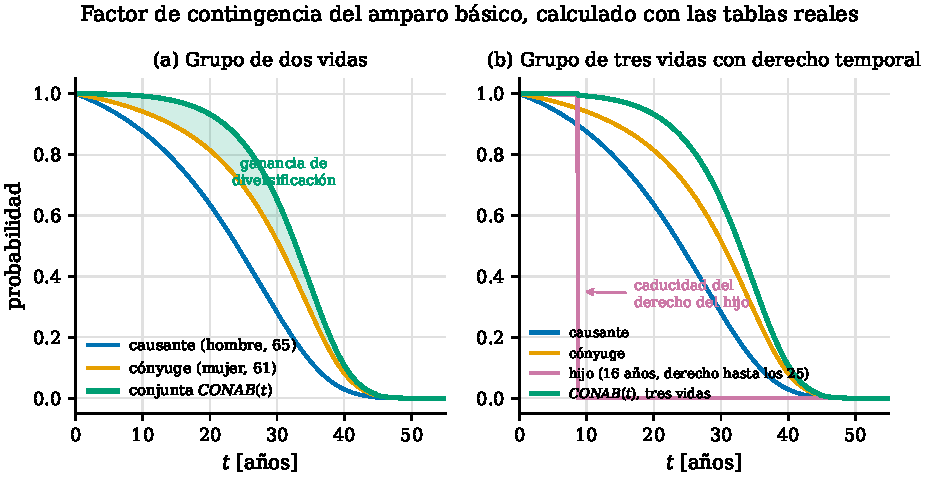
\includegraphics[width=\textwidth]{figuras/fig_supervivencia}
\caption[Factor de contingencia del amparo básico]{Supervivencia individual y
conjunta calculada con las tablas colombianas RV-08. La curva conjunta domina a
las individuales: el contrato dura, en esperanza, más que cualquiera de las vidas
por separado. En el panel (b), el derecho temporal del hijo caduca a los $25$ años
y su curva cae a cero, sin que $\CONAB$ se vea prácticamente afectado porque los
padres siguen vivos con alta probabilidad.}
\label{fig:supervivencia}
\end{figure}

\section{Descuento financiero}

Sea $i$ la tasa de interés técnico \emph{real} y $\{\pi^m_t\}$ la sucesión de
inflaciones mensuales implícitas del esquema de tres tramos. La tasa nominal
mensual del periodo $t$ es
\begin{equation}
\label{eq:tasa-nominal}
  j_t \;=\; (1+\pi^m_t)\,(1+\varepsilon_t)-1,
  \qquad
  \varepsilon_t=(1+\iota_t)^{1/12}-1,
\end{equation}
donde $\iota_t$ es la tasa \emph{forward} anual real obtenida de la curva
\emph{spot}\footnote{La relación telescópica entre tasas \emph{spot} y \emph{forward} es una identidad de no arbitraje, no una hipótesis de modelación: expresa que invertir a $t$ años debe rendir lo mismo que invertir a $t-1$ años y reinvertir un año más al tipo pactado hoy para ese periodo.} $\{i_t\}$ mediante la relación telescópica
$1+\iota_t=(1+i_t)^t/(1+i_{t-1})^{t-1}$. El factor de descuento acumulado es
\begin{equation}
\label{eq:descuento}
  v_t\;=\;\prod_{u=1}^{t-1}\frac{1}{1+j_u},\qquad v_1=1.
\end{equation}
Si la curva es plana, $i_t\equiv i$, entonces $\iota_t\equiv i$ y
\cref{eq:descuento} se reduce a la fórmula usual. La \cref{fig:descuento} muestra
la estructura temporal empleada.

\begin{figure}[H]
\centering
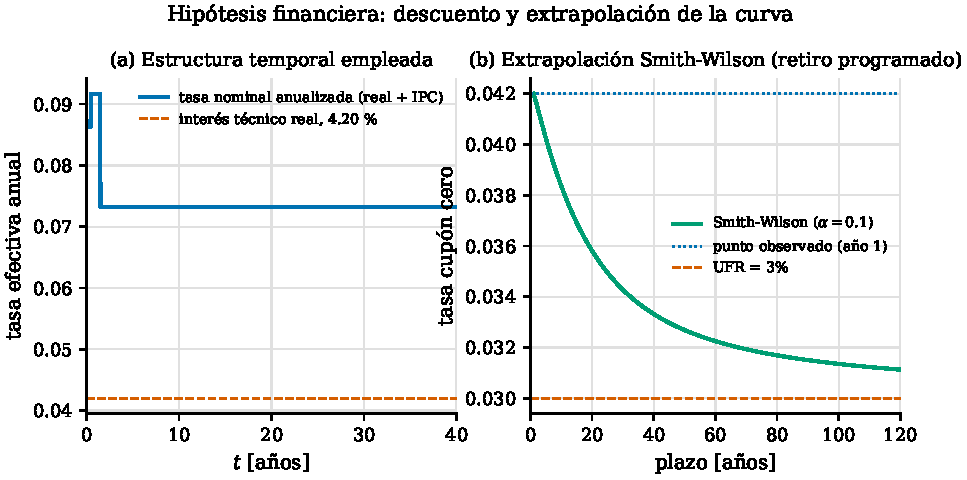
\includegraphics[width=\textwidth]{figuras/fig_descuento}
\caption[Estructura temporal de descuento]{Estructura temporal de tasas empleada
en la valoración. En el panel (a), la tasa nominal combina el interés técnico real
constante del \datoInteresRP\% con el esquema de inflación en tres tramos; la
transición entre tramos es visible en los primeros tres años. El panel (b) muestra
una ilustración de la extrapolación de Smith-Wilson, disponible en el motor
pero desactivada en la configuración de referencia
(\cref{cap:retiro}).}
\label{fig:descuento}
\end{figure}

\section{La función de valoración}

\subsection{Amparo básico}

Reuniendo \cref{eq:mesada-piso,eq:conab-modelo,eq:descuento} y aplicando el
\cref{cor:vp-renta}:
\begin{equation}
\label{eq:rab}
  \RAB(M)\;=\;\sum_{t=1}^{N}\max\{M\tau_t,\;S_t\}\;\nu_t\,\kappa_t\;\CONAB(t{+}1)\;v_{t+1}.
\end{equation}

\subsection{Auxilio funerario}

El auxilio funerario se paga al fallecimiento del causante y su cuantía es la
mesada vigente, acotada entre $5$ y $10$ salarios mínimos proyectados:
\begin{equation}
\label{eq:auf-cuantia}
  A_t(M)\;=\;
  \begin{cases}
    5S_t, & M_t(M)\le 5S_t,\\
    M_t(M), & 5S_t<M_t(M)\le 10S_t,\\
    10S_t, & M_t(M)>10S_t,
  \end{cases}
  \;=\;\med\bigl(5S_t,\;M_t(M),\;10S_t\bigr).
\end{equation}
Su valor presente actuarial es
\begin{equation}
\label{eq:auf}
  \AUF(M)\;=\;\sum_{t=1}^{N} A_t(M)\;\nu_t\;q^{(c)}_t\;\npx{t}{c}\;v_{t+1},
\end{equation}
donde $c$ denota al causante y $q^{(c)}_t$ su probabilidad de fallecimiento en el
mes $t$.

\begin{remark}
La forma $\med$ de \cref{eq:auf-cuantia} es la que produce la pérdida de
convexidad del \cref{thm:no-convexidad}. Obsérvese que el $\med$ actúa sobre
$M_t(M)$, que a su vez ya contiene un $\max$: la composición
$\med(5S_t,\max(M\tau_t,S_t),10S_t)$ es lineal a trozos con \emph{tres} quiebres
potenciales por periodo, aunque el primero de ellos, en $M\tau_t=S_t$, es inactivo
porque $S_t<5S_t$ y el $\med$ ya está saturado por abajo allí.
\end{remark}

\subsection{Recargos y reserva matemática}

Sea $\gamma$ el porcentaje de reserva por cambio de grupo y $g$ el de recargo de
gastos. Se define la \emph{base de reserva}
\begin{equation}
\label{eq:base}
  B(M)\;=\;(1+\gamma)\,\RAB(M)\;+\;\AUF(M),
\end{equation}
y la \emph{reserva matemática}, que es la función de valoración objeto de este
trabajo,
\begin{equation}
\label{eq:vp}
  \boxed{\;\VP(M)\;=\;\frac{B(M)}{1-g}\;=\;\frac{(1+\gamma)\,\RAB(M)+\AUF(M)}{1-g}.\;}
\end{equation}

La forma $B/(1-g)$ --- y no $B(1+g)$ ---\footnote{Con $g=0{,}05$, los factores son $1/(1-g)=1{,}0526316$ y $1+g=1{,}05$. La diferencia equivale aproximadamente al $0{,}263\%$ de la base $B$.} corresponde a que el recargo se define
como un porcentaje del \emph{total} y no de la base: si $R=B+gR$ entonces
$R=B/(1-g)$.

\begin{remark}[Reserva objetivo, prima y capital disponible]
En este trabajo $\VP$ designa la reserva objetivo calculada con el recargo
de gastos $g$. El motor distingue esta cantidad de la prima comercial,
que puede utilizar un recargo diferente. Por tanto, $\KA$ debe representar
el capital asignado a financiar la misma base de obligaciones y recargos
que contiene $\VP$. La igualdad $\VP(M)=\KA$ no identifica automáticamente
reserva matemática y prima comercial. La conciliación entre capital recibido,
gastos, reserva y prima requiere los términos de la nota técnica y del
contrato; no se presupone en el análisis numérico.
\end{remark}

\subsection{El problema de cotización}

\begin{definition}[Problema de cotización]
\label{def:problema}
Dado un capital $\KA>0$, hallar una mesada admisible $M^*\ge S_0$ tal que
\begin{equation}
\label{eq:problema}
  f(M^*)\;=\;\VP(M^*)-\KA\;=\;0.
\end{equation}
\end{definition}

Para estudiar la estructura de la valoración se utiliza también su extensión
a $M\ge0$, definida por las mismas fórmulas. La multiplicidad de raíces en
$[0,S_0]$ pertenece a ese dominio ampliado. En el dominio admisible, si
$\KA=\VP(S_0)$ y $\VP$ es estrictamente creciente por encima de $S_0$,
la solución es únicamente $M^*=S_0$.

\begin{remark}[Convención de signo]
El motor de producción define la función objetivo como $\KA-\VP(M)$, que es
\emph{no creciente}. En este trabajo se adopta la convención opuesta,
$f=\VP-\KA$, que es \emph{no decreciente} y estrictamente creciente por encima
de $S_0$, porque es la que permite aplicar sin cambios
de signo la teoría de métodos para funciones monótonas crecientes. La raíz es
evidentemente la misma.
\end{remark}

\section{Descomposición del valor presente}

La \cref{fig:flujos} descompone $\VP$ en sus tres factores para una póliza
concreta: la mesada proyectada, que crece con la indexación; el flujo esperado,
que es el producto de la mesada por la contingencia y por eso primero crece y
luego decae; y el flujo descontado, cuya área es exactamente $\VP$.

\begin{figure}[H]
\centering
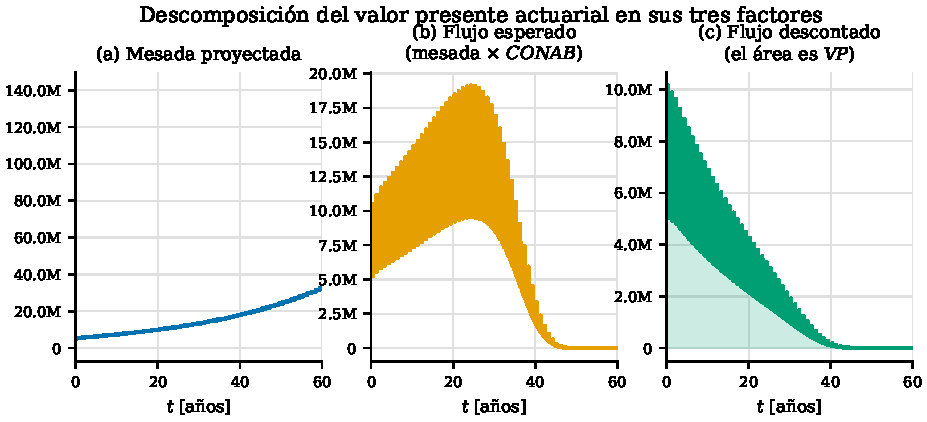
\includegraphics[width=\textwidth]{figuras/fig_flujos}
\caption[Descomposición del valor presente actuarial]{Descomposición del valor
presente actuarial. La forma del flujo descontado --- un máximo temprano seguido de
un decaimiento --- es la que determina la duración de Macaulay del contrato y, como
se verá en la \cref{sec:interpretacion-subdif}, la magnitud de la derivada
$\VP'$.}
\label{fig:flujos}
\end{figure}

\section{Forma canónica}

Todo el capítulo se resume en la siguiente observación, que es el punto de partida
del análisis estructural.

\begin{proposition}[Forma canónica de la función de valoración]
\label{prop:forma-canonica}
La función $\VP$ definida en \cref{eq:vp} admite la representación
\begin{equation}
\label{eq:canonica}
  \VP(M)\;=\;\sum_{t=1}^{N} w_t\,\max\{a_tM,\,b_t\}
            \;+\;\sum_{t=1}^{N} c_t\,\med\bigl(5b_t,\;a_tM,\;10b_t\bigr),
\end{equation}
con coeficientes
\begin{align*}
  w_t&=\frac{(1+\gamma)\,\nu_t\kappa_t\,\CONAB(t{+}1)\,v_{t+1}}{1-g}\ \ge 0,\\
  c_t&=\frac{\nu_t\,q^{(c)}_t\,\npx{t}{c}\,v_{t+1}}{1-g}\ \ge 0,
\end{align*}
\[
  a_t=\tau_t>0,\qquad b_t=S_t=S_0\phi_t>0,
\]
todos ellos \textbf{independientes de $M$}.
\end{proposition}
\begin{proof}
Sustitúyanse \cref{eq:rab,eq:auf} en \cref{eq:base,eq:vp} y agrúpense los factores
que no dependen de $M$. Para el segundo sumando obsérvese que
\[
\med(5S_t,\max(a_tM,b_t),10S_t)=\med(5b_t,a_tM,10b_t),
\]
ya que
$\max(a_tM,b_t)<5b_t$ si y solo si $a_tM<5b_t$ (porque $b_t<5b_t$), y análogamente
para la cota superior.
\end{proof}

La ecuación \cref{eq:canonica} exhibe a $\VP$ como una \emph{combinación cónica finita de
máximos y recortes de funciones afines}. Toda la estructura del problema está
contenida en esa frase, y el capítulo siguiente la desarrolla.

\chapter{Estructura de la ecuación de cotización}
\label{cap:estructura}

Este es el capítulo central del trabajo. Se establece aquí la estructura analítica
exacta de la función de valoración $\VP$ definida en \cref{eq:canonica}, y se
muestra que difiere en tres aspectos sustanciales de la que la práctica actuarial
supone. De esa estructura se derivan, en el \cref{cap:metodos}, las propiedades de
convergencia de los métodos iterativos.

A lo largo del capítulo se trabaja con la forma canónica
\begin{equation}
\label{eq:canonica-rep}
  \VP(M)\;=\;\underbrace{\sum_{t=1}^{N} w_t\,\max\{a_tM,\,b_t\}}_{\textstyle \VP_{\mathrm{ren}}(M)}
            \;+\;\underbrace{\sum_{t=1}^{N} c_t\,\med\bigl(5b_t,\;a_tM,\;10b_t\bigr)}_{\textstyle \VP_{\mathrm{auf}}(M)},
\end{equation}
con $w_t,c_t\ge0$ y $a_t,b_t>0$ independientes de $M$
(\cref{prop:forma-canonica}). Se supone en todo el capítulo que $w_1>0$, de modo que el primer periodo con $a_1=1$ y $b_1=S_0$ aporta positivamente a la renta.

\section{Regularidad básica}

\begin{proposition}[Continuidad y Lipschitz]
\label{prop:lipschitz}
$\VP$ es continua en $[0,\infty)$ y globalmente Lipschitz con constante
\[
  L \;=\; \sum_{t=1}^{N}\bigl(w_t+c_t\bigr)a_t \;<\;\infty .
\]
\end{proposition}
\begin{proof}
Cada $u\mapsto\max\{a_tu,b_t\}$ es $a_t$-Lipschitz y cada
$u\mapsto\med(5b_t,a_tu,10b_t)$ es también $a_t$-Lipschitz por el
\cref{lem:recorte}. La suma finita de funciones Lipschitz con pesos no negativos
$w_t,c_t$ es Lipschitz con constante la suma ponderada. La finitud de $L$ se sigue
de que $N=\datoNMeses$ es finito.
\end{proof}

Obsérvese que la finitud de $L$ no requiere ninguna hipótesis de convergencia de
series: es consecuencia directa del horizonte acotado
$\nu_t=0$ para $t\ge\datoVigenciaCorte$ de \cref{eq:vigencia}. Este es un punto
donde el modelo discreto real es \emph{más simple} que su idealización continua, y
donde el borrador original de este trabajo introducía hipótesis innecesarias\footnote{El borrador enunciaba un lema de convergencia absoluta de la serie que define el valor presente, con hipótesis de sumabilidad sobre los factores de descuento. Sobre una suma finita esas hipótesis son vacuas. Se conservan aquí, en cambio, las consecuencias: continuidad y carácter Lipschitz, que sí se usan.}.

\begin{proposition}[Linealidad a trozos]
\label{prop:pl}
$\VP$ es lineal a trozos en $[0,\infty)$, con a lo sumo
$3(\datoNAniosMax+1)=\datoNQuiebresMax$ puntos de quiebre.
\end{proposition}
\begin{proof}
Por el \cref{lem:pl-cerrado} la clase de funciones lineales a trozos es cerrada
bajo sumas finitas, $\max$ y $\min$; \cref{eq:canonica-rep} es una suma finita de
tales operaciones sobre funciones afines. La cota sobre el número de quiebres se
demuestra en el \cref{thm:quiebres}.
\end{proof}

\section{La región plana}

El primer resultado corrige el enunciado clásico de monotonía estricta.

\begin{theorem}[Región plana]
\label{thm:region-plana}
Sea $S_0$ el salario mínimo vigente. Entonces
\[
  \VP(M)\;=\;\VP(0)\;=\;\sum_{t=1}^N w_tb_t+5\sum_{t=1}^N c_tb_t
  \qquad\text{para todo } M\in[0,S_0].
\]
En particular $\VP$ \textbf{no} es estrictamente creciente en $[0,\infty)$, y
$\VP'\equiv0$ en el interior de $[0,S_0]$.
\end{theorem}
\begin{proof}
Sea $M\in[0,S_0]$ y $t\in\{1,\dots,N\}$ arbitrario. Como $\delta\ge0$, de
\cref{eq:factor-ipc} se sigue $\phi_{n}\ge\tau_{n}$ para todo $n\ge0$, y por tanto
$b_t=S_0\phi_t\ge S_0\tau_t\ge M\tau_t=a_tM$. Luego
\[
  \max\{a_tM,\,b_t\}=b_t ,
\]
independientemente de $M$. Para el término del auxilio funerario, de
$a_tM\le b_t<5b_t$ se obtiene
\[
  \med\bigl(5b_t,\,a_tM,\,10b_t\bigr)=5b_t ,
\]
también independiente de $M$. Sustituyendo ambos en \cref{eq:canonica-rep} se
obtiene la expresión del enunciado, constante en $M$.
\end{proof}

\begin{remark}[Lectura actuarial]
El resultado no es un artificio matemático: dice algo económicamente evidente una
vez enunciado. Si el capital solo alcanza para una mesada por debajo del salario
mínimo, la garantía legal obliga a pagar el salario mínimo de todos modos, de modo
que \emph{el costo del contrato deja de depender de la mesada nominal
contratada\footnote{Dicho de otro modo: por debajo del salario mínimo, la mesada contratada es una ficción contable. Lo que la aseguradora se obliga a pagar es el salario mínimo, y eso es lo que cuesta. La consecuencia matemática --- pérdida de inyectividad --- es el reflejo exacto de una consecuencia económica evidente una vez enunciada.}}. La función de valoración se satura, y con ella se pierde la
información necesaria para invertirla.
\end{remark}

\begin{corollary}[Condición de capital mínimo]
\label{cor:capital-minimo}
Sea $\KA_{\min}=\VP(S_0)$. En el dominio admisible $[S_0,\infty)$,
el problema tiene ninguna solución si $\KA<\KA_{\min}$,
la solución única $M=S_0$ si $\KA=\KA_{\min}$ y una solución única
$M>S_0$ si $\KA>\KA_{\min}$. En la extensión a $[0,\infty)$,
el caso de igualdad tiene como conjunto de soluciones $[0,S_0]$.
\end{corollary}
\begin{proof}
La región plana y la monotonía implican $\VP(M)\ge\KA_{\min}$.
La monotonía estricta en $[S_0,\infty)$ da la unicidad en la igualdad.
La existencia y unicidad por encima del mínimo se obtienen en el
\cref{thm:existencia} por continuidad y crecimiento no acotado.
\end{proof}

Para la póliza de referencia de este trabajo,
$\KA_{\min}=\datoKAmin$ pesos, es decir aproximadamente
$\datoKAminMill$ millones. La \cref{fig:region-plana} ilustra los tres casos.

\begin{figure}[H]
\centering
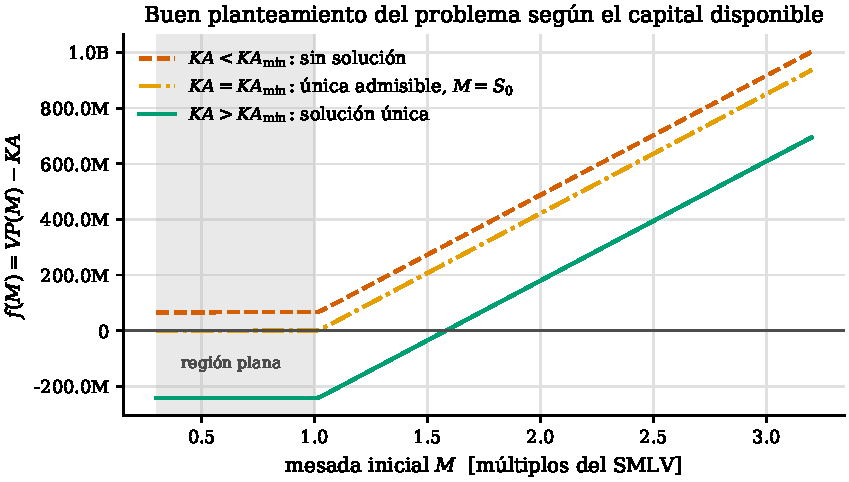
\includegraphics[width=.86\textwidth]{figuras/fig_region_plana}
\caption[Buen planteamiento del problema de cotización]{Los tres regímenes del
\cref{cor:capital-minimo}. Si el capital es insuficiente, $f$ no corta el eje y no
existe mesada admisible; si es exactamente el mínimo, $f$ se anula en todo el
intervalo $[0,\SMLV]$ de la extensión matemática. En el dominio admisible, la igualdad tiene la solución única $M=S_0$.}
\label{fig:region-plana}
\end{figure}

\begin{criticism}[Diagnóstico de insuficiencia y fallo numérico]
\label{crit:no-convergencia}
La implementación busca la raíz en $[S_0,25S_0]$. La insuficiencia
de capital debe diagnosticarse comparando $\KA$ con $\VP(S_0)$,
como establece el \cref{cor:capital-minimo}. El fracaso de un método
no basta para ese diagnóstico: también puede deberse a estancamiento
o a una raíz por encima del extremo superior. Devolver el salario mínimo
en tales situaciones no certifica la igualdad actuarial ni identifica
la financiación del importe pagado. La recomendación R1 exige separar
la inexistencia de una mesada financiable de los estados numéricos de
la búsqueda.
\end{criticism}

\section{Monotonía}

\begin{proposition}[Monotonía]
\label{prop:monotonia}
$\VP$ es no decreciente en $[0,\infty)$, y estrictamente creciente en
$[S_0,\infty)$.
\end{proposition}
\begin{proof}
La monotonía no estricta es inmediata: cada sumando de \cref{eq:canonica-rep} es no
decreciente en $M$ ($\max$ y $\med$ de funciones no decrecientes) y los pesos son
no negativos.

Para la monotonía estricta en $[S_0,\infty)$, sean $S_0\le M_1<M_2$. Considérese
el primer periodo, $t=1$, para el cual $n(1)=0$ y por tanto $a_1=\tau_1=1$,
$b_1=S_0\phi_1=S_0$. Entonces $a_1M_2=M_2>S_0=b_1$, luego
\[
  \max\{a_1M_2,b_1\}=M_2 \;>\; \max\{a_1M_1,b_1\}=\max\{M_1,S_0\}=M_1 ,
\]
donde la última igualdad usa $M_1\ge S_0$. Como $w_1>0$ por hipótesis y todos los
demás sumandos son no decrecientes, se concluye $\VP(M_1)<\VP(M_2)$.
\end{proof}

\begin{remark}
La prueba de monotonía estricta utiliza un término con peso positivo
del año calendario de valoración. En la derivada derecha en $S_0$
contribuyen todos los periodos con $n(t)=0$, no únicamente el primero.
Los periodos posteriores al primer reajuste tienen sus quiebres a la
derecha si $\delta>0$. La pendiente inmediatamente superior a $S_0$
es menor que la del tramo comercial, lo que hace más exigentes los
casos con capital cercano al mínimo.

\end{remark}

\section{El conjunto de puntos de quiebre}

\begin{theorem}[Caracterización de los quiebres]
\label{thm:quiebres}
Defínase, para $n=0,1,\dots,n_{\max}$ con
$n_{\max}=\lfloor(\datoVigenciaCorte-1)/12\rfloor=\datoNAniosMax$,
\[
  \rho_n \;=\; \frac{\phi_n}{\tau_n}\;=\;
  \begin{cases}
    1, & n=0,\\[2pt]
    \dfrac{1+\pi_1+\delta}{1+\pi_1}, & n=1,\\[4pt]
    \dfrac{(1+\pi_1+\delta)(1+\pi_2+\delta)}{(1+\pi_1)(1+\pi_2)}\,\rho^{\,n-2},
      & n\ge2,
  \end{cases}
  \qquad
  \rho\;=\;\frac{1+\pi_\infty+\delta}{1+\pi_\infty}.
\]
Entonces el conjunto de puntos de no diferenciabilidad de $\VP$ está contenido en
\begin{equation}
\label{eq:quiebres}
  \mathcal{B}\;=\;\underbrace{\bigl\{S_0\rho_n\bigr\}_{n=0}^{n_{\max}}}_{\text{racimo I}}
   \;\cup\;\underbrace{\bigl\{5S_0\rho_n\bigr\}_{n=0}^{n_{\max}}}_{\text{racimo II}}
   \;\cup\;\underbrace{\bigl\{10S_0\rho_n\bigr\}_{n=0}^{n_{\max}}}_{\text{racimo III}} .
\end{equation}
La sucesión $\{\rho_n\}$ es estrictamente creciente si $\delta>0$, con
$\rho_0=1$. Para la parametrización considerada,
$\rho_{n_{\max}}\approx\datoAnchoRacimo<2$; los tres racimos quedan
contenidos en los siguientes intervalos disjuntos:
\[
  \mathcal{B}\subset
  [S_0,\;\rho_{n_{\max}}S_0]\;\cup\;
  [5S_0,\;5\rho_{n_{\max}}S_0]\;\cup\;
  [10S_0,\;10\rho_{n_{\max}}S_0].
\]
\end{theorem}
\begin{proof}
Por el \cref{lem:pl-cerrado}, el conjunto de quiebres de la suma
\cref{eq:canonica-rep} está contenido en la unión de los conjuntos de quiebres de
sus sumandos. El sumando $t$-ésimo del primer bloque,
$M\mapsto\max\{a_tM,b_t\}$, tiene un único quiebre en $M=b_t/a_t$. El del segundo
bloque, $M\mapsto\med(5b_t,a_tM,10b_t)$, tiene dos, en $M=5b_t/a_t$ y
$M=10b_t/a_t$.

Ahora bien, $b_t/a_t = S_0\phi_t/\tau_t = S_0\rho_{n(t)}$ depende de $t$
\emph{únicamente a través del año calendario} $n(t)$, porque los factores de
indexación de \cref{eq:factor-ipc} se actualizan una vez al año.\footnote{Es el punto técnico decisivo de la demostración. Si la indexación fuese continua --- si la mesada creciera mes a mes en lugar de dar un salto anual --- habría un quiebre distinto por cada uno de los $\datoNMeses$ periodos, y el conjunto candidato seguiría siendo finito, aunque podría tener más elementos. La estructura discreta del reajuste es lo que hace tratable el problema.} Como
$\nu_t=0$ para $t\ge\datoVigenciaCorte$, los índices $t$ con peso no nulo
satisfacen $n(t)\le n_{\max}$. Esto da \cref{eq:quiebres}.

La monotonía estricta de $\rho_n$ para $\delta>0$ se sigue de que cada factor
$(1+\pi+\delta)/(1+\pi)>1$. Finalmente, los racimos son disjuntos porque
$\rho_{n_{\max}}<2$, luego
$\rho_{n_{\max}}S_0<5S_0$ y $5\rho_{n_{\max}}S_0<10S_0$.
\end{proof}

\begin{corollary}[Región afín]
\label{cor:region-afin}
$\VP$ es \textbf{afín} en cada uno de los intervalos
\[
  \bigl[\rho_{n_{\max}}S_0,\;5S_0\bigr],\qquad
  \bigl[5\rho_{n_{\max}}S_0,\;10S_0\bigr],\qquad
  \bigl[10\rho_{n_{\max}}S_0,\;\infty\bigr).
\]
\end{corollary}

El \cref{cor:region-afin} es el resultado con mayor consecuencia práctica de todo
el trabajo. El primero de esos intervalos, aproximadamente
$[1{,}15\,S_0,\;5\,S_0]$, contiene las mesadas de la muestra examinada: en los dos conjuntos reales del \cref{cap:resultados}
(\datoNReales{} cotizaciones de renta vitalicia y \datoNRealesRP{} registros
adicionales), todas las mesadas resultantes caen entre
$\datoMultMin$ y $\datoMultMax$ salarios mínimos, con media $\datoMultMedia$. Es
decir: \emph{el intervalo que contiene las mesadas de esta muestra es un tramo
afín}, y Newton con su pendiente exacta termina en un paso cuando el arranque también está en el interior de ese tramo. Así
ocurre (\cref{thm:terminacion-finita} y \cref{tab:terminacion}).

\begin{remark}[Por qué los racimos son tan estrechos]
La razón geométrica es $\rho=\datoRhoQuiebre$, esto es, un
$\datoRhoQuiebrePct\%$ anual: el deslizamiento $\delta=\datoDeslizamiento\%$ es
muy pequeño frente a la inflación de largo plazo $\pi_\infty=\datoIPClp\%$.
Acumulado sobre $\datoNAniosMax$ años produce apenas un ensanchamiento de
$\datoAnchoRacimo$. Si la política de salario mínimo fuese más agresiva --- un
deslizamiento de, digamos, $2\%$ anual --- los racimos se ensancharían hasta
solaparse, la región afín desaparecería y el problema numérico sería
sustancialmente más duro. La benignidad numérica del problema colombiano es, en
este sentido, una consecuencia contingente de su política salarial.\footnote{El experimento mental es verificable con la aplicación interactiva que acompaña a este trabajo: fijando el deslizamiento por encima del dos por ciento anual, los racimos se ensanchan hasta solaparse y la región afín comercial desaparece.}
\end{remark}

\begin{figure}[H]
\centering
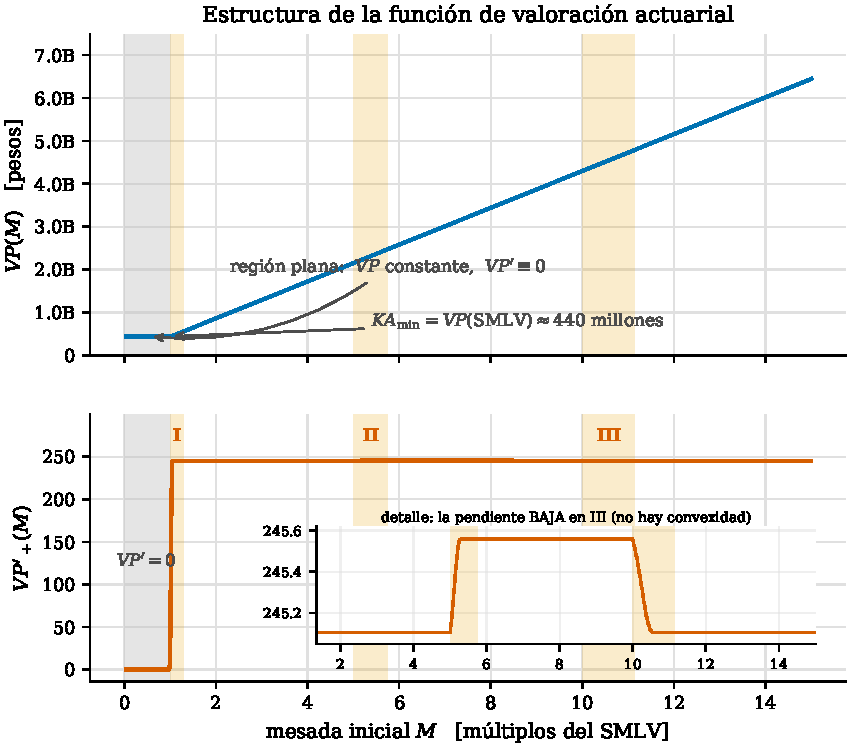
\includegraphics[width=.92\textwidth]{figuras/fig_estructura_vp}
\caption[Estructura de la función de valoración]{Estructura de $\VP$ y de su
derivada lateral derecha. Arriba: la función, con la región plana sombreada en
gris y los tres racimos de quiebres en naranja. Abajo: la derivada, que salta de
$0$ al valor de régimen en el racimo~I. El recuadro interior amplía la variación
fina de la pendiente y revela el hecho decisivo: en el racimo~III la pendiente
\emph{decrece}, lo que prueba que $\VP$ no es convexa
(\cref{thm:no-convexidad}).}
\label{fig:estructura}
\end{figure}

\begin{figure}[H]
\centering
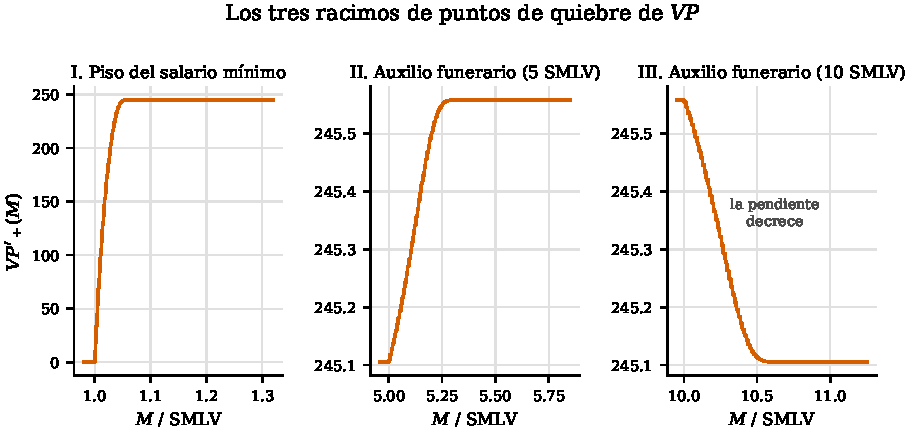
\includegraphics[width=\textwidth]{figuras/fig_zoom_quiebres}
\caption[Los tres racimos de quiebres]{Detalle de los tres racimos. En el
racimo~I la pendiente asciende desde $0$; en el II asciende de nuevo, al activarse
el auxilio funerario; en el III \emph{desciende}, al saturarse el tope de diez
salarios mínimos. Cada conjunto contiene a lo sumo $\datoNAniosMax+1$ quiebres candidatos, uno por año de proyección; los pesos nulos pueden eliminar saltos efectivos, con separaciones geométricas de razón $\datoRhoQuiebre$.}
\label{fig:zoom}
\end{figure}

\section{Convexidad: lo que se conserva y lo que se pierde}

\begin{proposition}[El amparo básico es convexo]
\label{prop:convexidad-rab}
$\VP_{\mathrm{ren}}$ es convexa en $[0,\infty)$.
\end{proposition}
\begin{proof}
Cada $M\mapsto\max\{a_tM,b_t\}$ es el máximo puntual de dos funciones afines,
luego convexo por el \cref{lem:preserva-convexidad}(a). La combinación cónica con
pesos $w_t\ge0$ preserva la convexidad por (b).
\end{proof}

\begin{theorem}[Pérdida de convexidad]
\label{thm:no-convexidad}
Si existe algún $t$ con $c_t>0$ --- es decir, si el contrato cubre auxilio
funerario --- entonces $\VP$ \textbf{no} es convexa en $[0,\infty)$. Concretamente,
la derivada lateral derecha satisface
\[
  \VP'_+\bigl(M\bigr) \;>\; \VP'_+\bigl(M'\bigr)
  \qquad\text{para } M\in\bigl(5\rho_{n_{\max}}S_0,\;10S_0\bigr),\;
  M'>10\rho_{n_{\max}}S_0 .
\]
\end{theorem}
\begin{proof}
Por el \cref{thm:subdiferencial} (que se demuestra a continuación y no depende de
este resultado), para $M$ en el intervalo indicado todos los términos del auxilio
funerario están activos, esto es $5b_t<a_tM<10b_t$ para todo $t$, y por tanto
\[
  \VP'_+(M)\;=\;\sum_t w_ta_t \;+\; \sum_t c_ta_t .
\]
Para $M'>10\rho_{n_{\max}}S_0$ se tiene $a_tM'>10b_t$ para todo $t$, de modo que
todos los términos del auxilio están saturados por arriba y su contribución a la
derivada es nula:
\[
  \VP'_+(M')\;=\;\sum_t w_ta_t .
\]
La diferencia es $\sum_t c_ta_t>0$ por hipótesis. Una función convexa tiene
derivada lateral derecha no decreciente\footnote{El resultado es estándar en análisis convexo; véase \citet[Teorema~24.1]{rockafellar1970} o \citet[§3.1]{boyd2004}. Su contrarrecíproco es lo que se usa aquí: exhibir dos puntos donde la derivada lateral derecha decrece basta para refutar la convexidad, sin necesidad de examinar la función en el resto del dominio.} \citep[Teorema 24.1]{rockafellar1970}; como
aquí decrece, $\VP$ no es convexa.
\end{proof}

Numéricamente, para la póliza de referencia la pendiente pasa de
$\datoPendienteAUF$ en la meseta intermedia a $\datoPendienteAfin$ por encima del
racimo~III: un descenso de $\datoSaltoAUF$ unidades. Es una violación pequeña en
magnitud relativa --- del orden de $2\cdot10^{-3}$ --- pero \emph{cualitativa}\footnote{El auxilio funerario representa una fracción muy pequeña del valor del contrato --- del orden del medio por ciento en la póliza de referencia --- de modo que su efecto sobre la pendiente es necesariamente pequeño. Lo que no es pequeño es su efecto sobre las propiedades cualitativas de la función.}: basta
para invalidar todo argumento que invoque convexidad\footnote{Conviene resistir la tentación de considerar despreciable una violación de dos milésimas. La convexidad es una propiedad cualitativa: o se tiene o no se tiene. Un argumento que la invoque es válido o inválido, y su conclusión no se vuelve \emph{casi} válida porque la violación sea pequeña. Lo que sí es legítimo decir --- y se dice en la \cref{sec:robustez-empirica} --- es que la consecuencia práctica observada es benigna.}.

\begin{criticism}[Consecuencia para la teoría de Newton]
\label{crit:convexidad}
El argumento clásico de convergencia monótona de Newton --- «si $f$ es convexa,
creciente y $x_0>x^*$, entonces $\{x_k\}$ decrece monótonamente hacia $x^*$» ---
descansa en que la tangente quede por debajo de la gráfica. En el racimo~III eso
falla, y la iteración puede sobrepasar la raíz. En la práctica el efecto es
pequeño en los experimentos, pero la hipótesis de convexidad deja de justificar
la convergencia monótona. Una garantía global se obtiene con la salvaguarda de
encaje y bisección periódica del \cref{alg:newton-salvaguardado}, bajo las
condiciones del \cref{thm:salvaguardado}. Este es
el argumento matemático que respalda la recomendación práctica de este trabajo.
\end{criticism}

\section{El subdiferencial y su interpretación actuarial}

\begin{theorem}[Subdiferencial exacto]
\label{thm:subdiferencial}
Para todo $M>0$, el $B$-subdiferencial de $\VP$ es
$\dB\VP(M)=\{\VP'_-(M),\;\VP'_+(M)\}$ con
\begin{align}
  \VP'_+(M) &= \sum_{t:\,a_tM\ge b_t} w_ta_t
             \;+\; \sum_{t:\,5b_t\le a_tM<10b_t} c_ta_t ,
  \label{eq:subdif-der}\\[2pt]
  \VP'_-(M) &= \sum_{t:\,a_tM> b_t} w_ta_t
             \;+\; \sum_{t:\,5b_t< a_tM\le 10b_t} c_ta_t ,
  \label{eq:subdif-izq}
\end{align}
y el subdiferencial de Clarke es
$\dC\VP(M)=\bigl[\min\{\VP'_-,\VP'_+\},\;\max\{\VP'_-,\VP'_+\}\bigr]$.
Si $M\notin\mathcal{B}$, ambos coinciden y $\VP$ es diferenciable en $M$ con
$\VP'(M)=\VP'_\pm(M)$.
\end{theorem}
\begin{proof}
La derivada lateral de $u\mapsto\max\{a_tu,b_t\}$ por la derecha vale $a_t$ si
$a_tu\ge b_t$ y $0$ si no; por la izquierda vale $a_t$ si $a_tu>b_t$ y $0$ si no.
Análogamente, para $u\mapsto\med(5b_t,a_tu,10b_t)$ la derivada por la derecha vale
$a_t$ si $5b_t\le a_tu<10b_t$ y $0$ en otro caso, y por la izquierda vale $a_t$ si
$5b_t<a_tu\le10b_t$. Las derivadas laterales de una suma finita son la suma de las
derivadas laterales; ponderando por $w_t,c_t$ se obtienen
\cref{eq:subdif-der,eq:subdif-izq}. La identificación con $\dB$ y $\dC$ es el
\cref{lem:subdif-pl}.
\end{proof}

\subsection{Qué significa la derivada}
\label{sec:interpretacion-subdif}

La expresión \cref{eq:subdif-der} no es una fórmula opaca. Sustituyendo los
coeficientes de la \cref{prop:forma-canonica}, en la región donde todos los
términos de renta están activos y ninguno del auxilio lo está,
\begin{equation}
\label{eq:derivada-anualidad}
  \VP'(M)\;=\;\frac{1+\gamma}{1-g}\sum_{t=1}^{N}
     \tau_t\,\nu_t\,\kappa_t\,\CONAB(t{+}1)\,v_{t+1}
  \;=\;\frac{1+\gamma}{1-g}\;\ddot a^{(\tau)}_{Y},
\end{equation}
donde $\ddot a^{(\tau)}_{Y}$ es exactamente el \textbf{factor de renta actuarial}
del grupo $Y$: el valor presente de una renta unitaria indexada, pagada
$\kappa_t$ veces por año mientras subsista el derecho.

\begin{aporte}
\textbf{Interpretación.} La derivada de la función de valoración respecto de la
mesada inicial \emph{es} el factor de renta del contrato, recargado por gastos y
cambio de grupo. En consecuencia:
\begin{itemize}[nosep,leftmargin=*]
  \item El paso de Newton $-f(M)/\VP'(M)$ tiene lectura financiera directa: es el
        exceso o defecto de capital dividido por el costo de un peso de mesada
        adicional. Es exactamente el ajuste que un actuario haría a mano.
  \item El subgradiente nunca se anula por encima del salario mínimo, porque es
        una suma de factores de renta estrictamente positivos. Esta es la
        $BD$-regularidad del \cref{thm:bd-regularidad}.
  \item Los dos elementos de $\dB\VP$ en un quiebre corresponden a incluir o
        excluir del factor de renta los periodos en que la mesada está exactamente
        sobre el piso legal.
\end{itemize}
\end{aporte}

Para la póliza de referencia, $\VP'=\datoPendienteAfin$: cada peso adicional de
mesada mensual cuesta $\datoPendienteAfin$ pesos de capital. Recíprocamente, cada
millón de pesos adicional de capital compra $\datoCondicionamientoInverso$ pesos
más de mesada mensual.

\section{Existencia, unicidad y condicionamiento}

\begin{theorem}[Existencia y unicidad en el dominio admisible]
\label{thm:existencia}
En $[S_0,\infty)$ existe una solución única si y solo si
$\KA\ge\KA_{\min}=\VP(S_0)$. En la igualdad es $M^*=S_0$;
para capital estrictamente superior se tiene $M^*>S_0$.
\end{theorem}
\begin{proof}
La función es continua y estrictamente creciente en $[S_0,\infty)$.
Para $M>\rho_{n_{\max}}S_0$, la contribución de renta tiene pendiente
$\sum_t w_ta_t>0$, mientras que el auxilio es no decreciente.
Por tanto $\VP(M)\to\infty$ y su imagen en ese dominio es
$[\VP(S_0),\infty)$. La continuidad da existencia y la monotonía
estricta da unicidad.
\end{proof}

\begin{remark}[Dominio y condición de capital]
La igualdad $\VP(0)=\VP(S_0)$ hace numéricamente equivalentes las
condiciones $\VP(0)<\KA$ y $\VP(S_0)<\KA$. La región plana impide
utilizar monotonía estricta en todo $[0,\infty)$, pero no altera esa
desigualdad. La multiplicidad en la igualdad corresponde al dominio
ampliado; en el dominio admisible la mesada mínima es única.
\end{remark}

\begin{theorem}[Estabilidad de Lipschitz y condicionamiento]
\label{thm:condicionamiento}
Sea $m=\inf\{\,V : V\in\dB\VP(M),\ M\ge \rho_{n_{\max}}S_0\,\}>0$. Para capitales
$\KA_1,\KA_2>\KA_{\min}$ con soluciones
$M_1^*,M_2^*\ge\rho_{n_{\max}}S_0$,
\[
  \bigl|M_1^*-M_2^*\bigr|\;\le\;\frac{1}{m}\,\bigl|\KA_1-\KA_2\bigr| .
\]
Si $M^*$ está en el interior de un tramo afín, el número de condición
relativo del problema es
\[
  \kappa_{\mathrm{rel}}
  \;=\;\frac{\KA}{M^*}\cdot\left|\frac{dM^*}{d\KA}\right|
  \;=\;\frac{\VP(M^*)}{M^*\,\VP'(M^*)} .
\]
\end{theorem}
\begin{proof}
Por el teorema del valor medio para funciones Lipschitz\footnote{Véase \citet[Teorema~2.3.7]{clarke1983}. El enunciado sustituye la derivada del teorema del valor medio clásico por un elemento del subdiferencial de Clarke, y es precisamente la herramienta que permite hacer análisis de estabilidad sobre funciones no diferenciables.}
\citep[Teorema 2.3.7]{clarke1983}, $\KA_2-\KA_1=\VP(M_2^*)-\VP(M_1^*)=V(M_2^*-M_1^*)$
para algún $V\in\dC\VP$ en el segmento, y $V\ge m$. La expresión del número de
condición es la definición usual aplicada a $M^*=\VP^{-1}(\KA)$, cuya derivada es
$1/\VP'(M^*)$ por el teorema de la función inversa, válido porque $\VP$ es afín en
un entorno.
\end{proof}

Para la póliza de referencia, $\kappa_{\mathrm{rel}}=\datoCondRelativa$. Es decir:
\emph{el problema está esencialmente perfectamente condicionado}. Un error
relativo en el capital se traslada casi exactamente, sin amplificación, a un error
relativo en la mesada. Este buen condicionamiento facilita resolver el problema,
pero no garantiza por sí solo que todo método alcance precisión de máquina:
también intervienen su convergencia, las tolerancias y el redondeo. La comparación
de métodos debe contrastar la exactitud alcanzada con el costo de obtenerla.

\section{Semisuavidad y regularidad}

\begin{theorem}[Semisuavidad fuerte]
\label{thm:semisuavidad}
$f=\VP-\KA$ es fuertemente semisuave en todo punto de $[0,\infty)$. Más aún, para
$M\notin\mathcal{B}$ y $|d|$ menor que la distancia de $M$ a $\mathcal{B}$, el
residuo semisuave es \emph{exactamente cero}.
\end{theorem}
\begin{proof}
Es el \cref{lem:pl-semisuave} aplicado a $f$, que es lineal a trozos por la
\cref{prop:pl} con conjunto finito de quiebres $\mathcal{B}$ (\cref{thm:quiebres}).
\end{proof}

\begin{theorem}[$BD$-regularidad]
\label{thm:bd-regularidad}
Sea $M^*>S_0$ una solución. Todo $V\in\dB f(M^*)$ satisface
$V\ge w_1a_1>0$; por tanto $f$ es $BD$-regular en $M^*$.
Si además $M^*>\rho_{n_{\max}}S_0$, se obtiene la cota más fuerte
$V\ge\sum_t w_ta_t>0$.
\end{theorem}
\begin{proof}
Para $M^*>S_0$, el primer término está activo con desigualdad estricta en ambas derivadas, lo que da la primera cota. Para la segunda, ambas derivadas contienen el sumando
$\sum_{t:\,a_tM^*\ge b_t}w_ta_t$ (respectivamente con desigualdad estricta). Como
$M^*>\rho_{n_{\max}}S_0=\max_n b_t/a_t$, todos los índices $t$ están activos con
desigualdad estricta, luego ambas derivadas laterales valen al menos
$\sum_tw_ta_t$. Esta cantidad es positiva porque $w_1>0$ y $a_1=1$.
\end{proof}

\begin{corollary}
\label{cor:qi-sun-aplica}
Para $M^*>S_0$ se cumplen las hipótesis del \cref{thm:qi-sun}; el error
del método de Newton semisuave satisface localmente una cota cuadrática.
Además, como hay un número finito de quiebres, un arranque suficientemente
próximo selecciona un tramo cuya clausura contiene la raíz. El apartado (i)
del \cref{thm:terminacion-finita} da entonces terminación en un paso en
aritmética exacta. Esta terminación local no se interpreta como un orden
asintótico exacto con constante positiva.
\end{corollary}

\begin{remark}[El caso $M^*$ dentro del racimo~I]
Si la solución cae \emph{dentro} del racimo~I --- lo que ocurre cuando el capital
apenas supera el mínimo ---, la $BD$-regularidad sigue valiendo pero con una cota
$m$ mucho menor, pues solo una fracción de los periodos está activa. Es el caso
numéricamente más exigente y el que se aísla en el escenario \texttt{R2} de los
experimentos.
\end{remark}

\section{Un detalle de implementación con consecuencias analíticas}

\begin{proposition}[La distinción de casos es inocua en valor, no en derivada]
\label{prop:continuidad-rama}
Sea $\widetilde{\VP}$ la función definida como $\VP$ salvo que en $M=S_0$ se usa
$\phi_t$ en lugar de $\tau_t$ como factor de crecimiento de la mesada (la
distinción de casos de la \cref{rem:rama-smlv}). Entonces
$\widetilde{\VP}=\VP$ en todo $[0,\infty)$, pero la derivada lateral derecha
calculada con la fórmula \cref{eq:subdif-der} evaluada sobre la rama $\phi$ en
$M=S_0$ difiere de $\VP'_+(S_0)$.
\end{proposition}
\begin{proof}
En $M=S_0$, la rama $\phi$ da $\max\{S_0\phi_t,S_0\phi_t\}=S_0\phi_t=b_t$, y la
rama $\tau$ da $\max\{S_0\tau_t,S_0\phi_t\}=b_t$ porque $\phi_t\ge\tau_t$. Los
valores coinciden, luego $\widetilde{\VP}(S_0)=\VP(S_0)$; fuera de $M=S_0$ las
definiciones son idénticas. Para la derivada, la fórmula \cref{eq:subdif-der}
aplicada con $a_t=\phi_t$ activa \emph{todos} los índices, pues
$S_0\phi_t\ge b_t=S_0\phi_t$ con igualdad, y devuelve $\sum_tw_t\phi_t$; en cambio
la derivada lateral derecha verdadera se calcula sobre la rama $\tau$ y solo
activa los índices con $S_0\tau_t\ge S_0\phi_t$, es decir únicamente $n(t)=0$.
\end{proof}

Numéricamente, la fórmula ingenua devuelve $249{,}06$ en $M=S_0$ frente al valor
correcto $7{,}23$: un factor de $34$\footnote{El valor correcto de la derivada lateral derecha en $M=S_0$ es $7{,}23$, y corresponde a los pocos periodos del año calendario de la valoración en los que el piso aún no se ha separado del nominal. La fórmula evaluada sobre la rama equivocada devuelve $249{,}06$, que es la pendiente que tendría la función si todos los periodos estuviesen activos.}. Un método de Newton que arranque exactamente
en el salario mínimo daría, con la fórmula ingenua, un paso $34$ veces menor del
debido. La implementación de este trabajo corrige el punto seleccionando la rama
$\tau$ para el cálculo de la derivada (recomendación~R2 de la
\cref{sec:hallazgos-codigo}).

\section{Verificación numérica de la estructura}

Los resultados anteriores se contrastaron numéricamente sobre la póliza de
referencia. El \cref{tab:verificacion-estructura} resume esos contrastes, que
ilustran las demostraciones sin sustituirlas.

\begin{table}[H]
\centering
\caption[Verificación numérica de la estructura]{Verificación numérica de los
resultados estructurales sobre la póliza de referencia (hombre de 65 años con
cónyuge de 61, capital \$\,\datoCapitalEjemplo).}
\label{tab:verificacion-estructura}
\small
\begin{tabular}{@{}p{5.6cm}p{4.2cm}p{4.4cm}@{}}
\toprule
\textbf{Resultado} & \textbf{Predicción} & \textbf{Verificación} \\
\midrule
\cref{thm:region-plana}: región plana &
$\VP$ constante en $[0,S_0]$ &
$\VP$ idéntica a $12$ cifras en $M/S_0\in\{0{,}01;\dots;1\}$ \\
\cref{cor:capital-minimo}: capital mínimo &
$\KA_{\min}=\VP(S_0)$ &
$\datoKAmin$ pesos \\
\cref{thm:quiebres}: tres racimos &
$[1;\datoAnchoRacimo]$, $[5;5\cdot\datoAnchoRacimo]$, $[10;10\cdot\datoAnchoRacimo]$ en unidades de $S_0$ &
saltos de $\VP'$ detectados solo en esos tres intervalos
(\cref{fig:zoom}) \\
\cref{cor:region-afin}: región afín &
$\VP(M+d)=\VP(M)+\VP'\!\cdot d$ exacto &
error relativo del orden de $10^{-16}$ para $M\in\{3;6;30\}$ millones \\
\cref{thm:no-convexidad}: no convexidad &
$\VP'$ decrece tras el racimo~III &
$\datoPendienteAUF\to\datoPendienteAfin$ \\
\cref{thm:subdiferencial}: subdiferencial &
coincide con la diferencia central &
coincidencia a $10$ cifras fuera de $\mathcal{B}$ \\
\cref{thm:condicionamiento}: condicionamiento &
$\kappa_{\mathrm{rel}}\approx1$ &
$\datoCondRelativa$ \\
\bottomrule
\end{tabular}
\end{table}

La \cref{fig:residuo-lineal} ofrece la síntesis visual del capítulo. A escala
natural $\VP$ es indistinguible de una recta; restándole la cuerda que une sus
extremos, la estructura lineal a trozos aparece con toda claridad, y su amplitud
relativa resulta ser del orden de $10^{-3}$. El problema es genuinamente no suave
y, al mismo tiempo, genuinamente benigno: ambas cosas a la vez, y esa combinación
es precisamente lo que explica los resultados del \cref{cap:resultados}.

\begin{figure}[H]
\centering
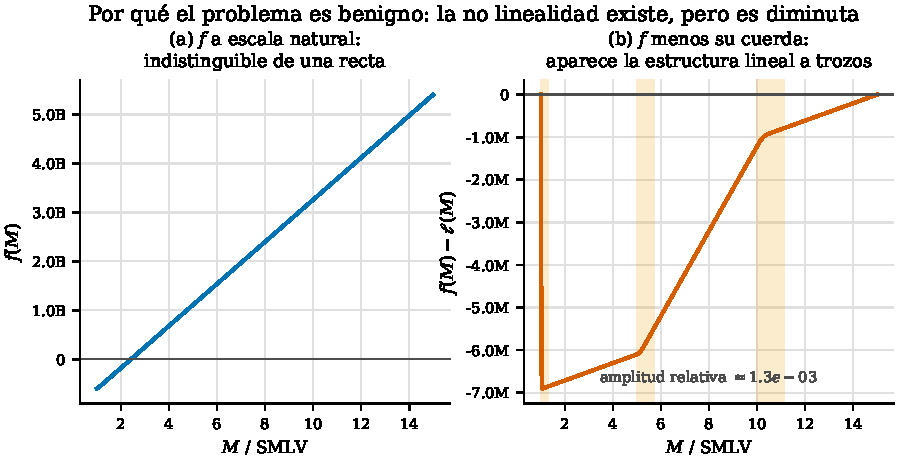
\includegraphics[width=\textwidth]{figuras/fig_residuo_lineal}
\caption[La no linealidad amplificada]{Síntesis del capítulo. A la izquierda, $f$
tal como se ve: una recta. A la derecha, $f$ menos su cuerda, que amplifica la
estructura por un factor de mil y revela los tres racimos de quiebres del
\cref{thm:quiebres} exactamente donde la teoría los predice.}
\label{fig:residuo-lineal}
\end{figure}

\chapter{Métodos numéricos iterativos}
\label{cap:metodos}

Este capítulo presenta los \datoNMetodos{} métodos que se comparan en el trabajo.
Para cada uno se enuncia la iteración, se establece su orden de convergencia
teórico y se analiza \emph{qué le ocurre sobre el problema concreto} del \cref{cap:estructura}. Este último punto es el que da contenido al capítulo: sobre
una función lineal a trozos, varios métodos pueden terminar en pocos pasos, y
su comportamiento se explica mejor por la estructura del problema que por el
orden asintótico que les asigna la teoría genérica.

Los métodos se agrupan en tres familias según la información que utilizan y la
garantía que ofrecen.

\begin{table}[H]
\centering
\caption[Taxonomía de los métodos]{Taxonomía de los métodos comparados. La columna
$c$ indica el costo nominal por iteración; para los métodos analíticos supone
una obtención conjunta de valor y derivada. $E=p^{1/c}$ es el índice de
eficiencia de Ostrowski (\cref{def:ostrowski}); el costo efectivo incluye todas
las llamadas al motor.}
\label{tab:taxonomia}
\small
\begin{tabular}{@{}llccc l@{}}
\toprule
\textbf{Familia} & \textbf{Método} & \textbf{$p$} & \textbf{$c$} & \textbf{$E$} & \textbf{Garantía} \\
\midrule
\multirow{8}{*}{Encaje}
 & Bisección          & $1$      & $1$ & $1{,}000$ & global, solo continuidad \\
 & Regula falsi       & $1$      & $1$ & $1{,}000$ & global \\
 & Illinois           & $1{,}442$& $1$ & $1{,}442$ & global \\
 & Pegasus            & $1{,}642$& $1$ & $1{,}642$ & global \\
 & Anderson--Björck   & $1{,}710$& $1$ & $1{,}710$ & global \\
 & Ridders            & $2$      & $2$ & $1{,}414$ & global \\
 & Brent              & superlineal& $1$ & --- & global, con encaje \\
 & ITP                & $1{,}618$& $1$ & $1{,}618$ & global, peor caso óptimo \\
\midrule
\multirow{9}{*}{Abiertos}
 & Secante            & $1{,}618$& $1$ & $1{,}618$ & local \\
 & Newton (dif.\ fin.)& $2$      & $3$ & $1{,}260$ & local \\
 & Newton (analítico) & $2$      & $1$ & $2{,}000$ & local \\
 & Steffensen         & $2$      & $2$ & $1{,}414$ & local \\
 & Steffensen escalado& $2$      & $2$ & $1{,}414$ & local \\
 & Müller             & $1{,}839$& $1$ & $1{,}839$ & local \\
 & Halley             & $3$      & $3$ & $1{,}442$ & local \\
 & Punto fijo relajado& $1$      & $1$ & $1{,}000$ & local, contracción \\
 & Aitken--Steffensen & $2$      & $2$ & $1{,}414$ & local \\
\midrule
\multirow{2}{*}{No suaves}
 & Newton semisuave   & $2$      & $1$ & $2{,}000$ & local, $BD$-regularidad \\
 & Newton salvaguardado& finito local& $1$ & --- & global; bisección periódica \\
\bottomrule
\end{tabular}
\end{table}

\section{Marco general y criterios de comparación}

\subsection{El costo relevante}

\begin{remark}[Por qué se cuentan evaluaciones y no iteraciones]
\label{rem:costo}
Una llamada al motor construye la proyección actuarial de $\datoNMeses$
periodos y domina el costo de las pocas operaciones escalares de la iteración.
La medida principal de trabajo es, por ello, el número de llamadas efectivas
al motor, junto con el tiempo medido. Deben incluirse las llamadas que
obtienen derivadas y las que preparan parámetros de relajación. El costo
nominal de Newton analítico es una llamada por punto solo cuando valor y
derivada se calculan conjuntamente y se reutilizan; si se calculan por
separado, ambas llamadas se contabilizan. La secante necesita un nuevo valor
por paso y Newton con diferencias centradas requiere, en general, tres.
\end{remark}

La instrumentación memoiza los valores ya calculados por punto. Una consulta
resuelta desde esa memoria no constituye una nueva ejecución del motor. La
misma convención debe aplicarse a todos los métodos y a la preparación que
cada uno necesita.

\subsection{Criterios de parada y el desajuste dimensional}
\label{sec:parada}

La tolerancia del residuo se expresa en unidades de capital. En los métodos
con encaje también puede certificarse el error mediante el ancho del intervalo:
\begin{equation}
\label{eq:parada}
  |f(x_k)|<\varepsilon_f
  \qquad\text{o, con encaje válido,}\qquad
  \frac{b_k-a_k}{2}\le\varepsilon_x ,
\end{equation}
devolviendo en el segundo caso el punto medio del intervalo. Un paso pequeño
$|x_k-x_{k-1}|$ se utiliza como diagnóstico de estancamiento; por sí solo no
certifica una raíz, pues un recorte al dominio puede producir un paso nulo
con residuo no nulo.

\begin{criticism}[Conversión del residuo en error de mesada]
\label{crit:parada}
El motor de producción utiliza una tolerancia de
$\varepsilon_f=\datoEpsilonProd$ peso de capital. Para relacionarla con la
exactitud de la mesada, supóngase que las pendientes de $\VP$ en el intervalo
que une $x$ con $M^*$ están acotadas inferiormente por $m>0$. Entonces
\[
  |x-M^*|\le\frac{|f(x)|}{m}.
\]
En un mismo tramo afín puede tomarse $m=\VP'$, de modo que la pendiente
$\datoPendienteAfin$ convierte un residuo de un peso en un error de mesada del
orden de $4\cdot10^{-3}$ pesos. Para garantizar una tolerancia de mesada
$\varepsilon$, es suficiente exigir $|f(x)|\le m\varepsilon$. Si se atraviesan
quiebres, la derivada en un único punto no sustituye necesariamente a esa cota
inferior. La recomendación~R3 de la \cref{sec:hallazgos-codigo} consiste en
declarar las unidades de la tolerancia y certificar su conversión mediante
una cota válida o mediante el encaje.
\end{criticism}

\section{Métodos con encaje}

Todos comparten la hipótesis inicial $f(a)f(b)<0$ y la propiedad invariante de
mantener un intervalo que contiene una raíz. Su virtud común es que la garantía de
convergencia \emph{no usa diferenciabilidad}, y por tanto sobrevive intacta a la
estructura no suave de $\VP$.

\subsection{Bisección}

\begin{algorithm}[H]
\caption{Bisección}
\label{alg:biseccion}
\SetAlgoLined
\KwIn{$f$, $[a,b]$ con $f(a)f(b)<0$, tolerancias}
\While{no se cumpla \cref{eq:parada}}{
  $x\leftarrow (a+b)/2$\;
  \eIf{$f(a)f(x)<0$}{$b\leftarrow x$}{$a\leftarrow x$, $f(a)\leftarrow f(x)$}
}
\KwOut{$x$}
\end{algorithm}

Su análisis es el \cref{thm:cota-biseccion}. Sobre el problema de este trabajo, con
$[a,b]=[S_0,25S_0]$ y $\varepsilon_x=10^{-8}$, la cota da
$\lceil\log_2(24S_0/10^{-8})\rceil\approx52$ iteraciones. Con la tolerancia de
producción en el residuo el número observado es $\datoEvBis$ evaluaciones en
promedio\footnote{La discrepancia entre la cota teórica de unas cincuenta y dos iteraciones y las treinta y tres observadas se explica porque el criterio de parada efectivo es el del residuo y no el del paso: con una pendiente de $\datoPendienteAfin$, un residuo menor que un peso corresponde a un error en la mesada del orden de $4\cdot10^{-3}$ pesos, muy por encima de la tolerancia $\varepsilon_x=10^{-8}$ que da lugar a la cota.}.

\begin{remark}[Una advertencia metodológica]
\label{rem:sesgo-diadico}
Un detalle del diseño experimental resulta crucial. Si la raíz se sitúa en un
múltiplo «redondo» del salario mínimo, los puntos medios sucesivos de la bisección
pueden coincidir \emph{exactamente} con ella por pura aritmética del encaje. En una
versión preliminar de los experimentos, con objetivos en $2{,}5$ y $5{,}0$
salarios mínimos, la bisección aparentaba converger en $6$ evaluaciones ---
compitiendo con Newton --- por este artefacto. Los escenarios definitivos usan
multiplicadores irracionales (por ejemplo, $1+\sqrt2$ y $3+\sqrt5$) para
reducir ese sesgo. El efecto sobre la conclusión es grande: el costo medio
de la bisección pasa de $21{,}6$ a $\datoEvBis$ evaluaciones\footnote{Se documenta este episodio porque ilustra un riesgo metodológico general en la comparación de algoritmos: los conjuntos de prueba construidos con valores «redondos» pueden favorecer sistemáticamente a los métodos cuya aritmética coincide con esa forma de redondeo. La bisección, que divide en potencias de dos, es especialmente vulnerable a ello.}.
\end{remark}

\subsection{Regula falsi y sus correcciones}

La regula falsi sustituye el punto medio por la raíz de la cuerda:
\begin{equation}
\label{eq:regula}
  x \;=\; b - f(b)\,\frac{b-a}{f(b)-f(a)} .
\end{equation}

\begin{proposition}[Estancamiento de la regula falsi]
\label{prop:estancamiento}
Si $f$ es continua, estrictamente convexa y estrictamente creciente en $[a,b]$,
con $f(a)<0<f(b)$, el extremo $b$ se conserva en las iteraciones exactas
de regula falsi y el ancho del encaje tiende a $b-x^*>0$. Si además $f$ es
continuamente diferenciable en un entorno de la raíz y $f'(x^*)>0$, la
convergencia es lineal con razón
$R=1-f'(x^*)(b-x^*)/f(b)\in(0,1)$.
\end{proposition}
\begin{proof}
La convexidad estricta sitúa la gráfica estrictamente por debajo de la
cuerda en el interior. En la raíz de la cuerda se tiene, por tanto,
$f(x)<0$ y se actualiza $a\leftarrow x$. El extremo derecho se conserva.
La sucesión de extremos izquierdos crece hacia la raíz y su límite da
el ancho indicado. La linealización de \cref{eq:regula} respecto del
extremo izquierdo en $x^*$ proporciona $R$. La pendiente de la cuerda
entre $x^*$ y $b$ es estrictamente mayor que $f'(x^*)$, de donde
$0<R<1$. Con convexidad no estricta puede haber tramos afines y
terminación exacta; ese caso no implica estancamiento asintótico.
\end{proof}

En el modelo afín a trozos, la conservación de un extremo puede coexistir
con una buena reducción del residuo. Deben distinguirse el ancho del
encaje y el error del punto propuesto; la proposición anterior no se aplica
como una hipótesis de convexidad estricta global a $\VP$.

Las tres correcciones clásicas atacan el estancamiento reduciendo por un factor
$\gamma$ el valor de $f$ en el extremo retenido:
\begin{align*}
  \text{Illinois:}&\quad \gamma=\tfrac12,\\
  \text{Pegasus:}&\quad \gamma=\frac{f(b)}{f(b)+f(x)},\\
  \text{Anderson--Björck:}&\quad \gamma=\max\Bigl\{1-\frac{f(x)}{f(b)},\ \tfrac12\Bigr\}.
\end{align*}
Los órdenes resultantes son $1{,}442$, $1{,}642$ y $1{,}710$ respectivamente
\citep{dowell1972,anderson1973}, con una sola evaluación por paso: son, en
términos del índice de Ostrowski, de los métodos más eficientes del catálogo entre
los que conservan garantía global.

\begin{remark}
La coincidencia de conteos medios entre variantes no implica que sus
sucesiones de iterados sean idénticas. La estructura afín explica que las
diferencias puedan ser pequeñas: cuando los dos puntos que definen la
cuerda pertenecen al mismo tramo que contiene la raíz, la interpolación
lineal es exacta. Fuera de esa situación deben contrastarse las
trayectorias, además de sus conteos agregados.
\end{remark}

\subsection{Ridders}

Supone que $g(x)=f(x)e^{Q(x-x_1)}$ es lineal para un $Q$ adecuado. Evaluando en el
punto medio $x_2$ y despejando se obtiene
\begin{equation}
\label{eq:ridders}
  x_3 \;=\; x_2 + (x_2-a)\,\frac{\sgn\bigl(f(a)-f(b)\bigr)\,f(x_2)}
                                {\sqrt{f(x_2)^2-f(a)f(b)}} .
\end{equation}
El iterado $x_3$ siempre cae dentro de $[a,b]$, de modo que conserva el encaje, y
la convergencia es cuadrática por \emph{par} de evaluaciones, es decir de orden
$\sqrt2$ por evaluación \citep{ridders1979}.

\subsection{Brent}

Combina interpolación cuadrática inversa, secante y bisección, aceptando el
candidato interpolado solo si satisface condiciones de progreso
\citep{brent1973}. Conserva el encaje y presenta convergencia superlineal en
el caso regular. La interpolación no implica que el número de iteraciones
coincida con la cota de la bisección en todo problema. Se utiliza como
referencia de un método híbrido disponible en bibliotecas científicas, como
\texttt{scipy.optimize.brentq}.

\subsection{ITP}

El método \emph{Interpolate--Truncate--Project} \citep{oliveira2021} es el
resultado más reciente del catálogo. En cada iteración:
\begin{enumerate}[nosep,leftmargin=*]
  \item \textbf{Interpolar:} calcular el candidato de regula falsi $x_f$.
  \item \textbf{Truncar:} desplazarlo hacia el punto medio a lo sumo
        $\delta=\kappa_1|b-a|^{\kappa_2}$, obteniendo $x_t$.
  \item \textbf{Proyectar:} proyectar $x_t$ sobre el intervalo minmax
        $[x_{1/2}-r,\;x_{1/2}+r]$ con
        $r=\varepsilon 2^{n_{\max}-j}-\tfrac12(b-a)$.
\end{enumerate}
La etapa 3 es la que garantiza que ITP nunca gaste más de $n_0$ iteraciones
adicionales sobre la cota de la bisección\footnote{El resultado de \citet{oliveira2021} es notable porque durante décadas se consideró que la optimalidad en el peor caso y la convergencia superlineal eran objetivos incompatibles: los métodos rápidos degradaban en el peor caso y los robustos no aceleraban en el caso bueno. ITP alcanza ambas.}, y --- punto clave para este trabajo ---
esa garantía no usa diferenciabilidad, luego sobrevive en los quiebres.

\begin{remark}[Por qué ITP resulta caro aquí]
Los experimentos muestran que ITP requiere $\datoEvITP$ evaluaciones, muy por
encima de Brent. No es un defecto del método sino del ajuste de sus parámetros: la
etapa de proyección está calibrada para \emph{garantizar} el peor caso, y con el
intervalo de partida $[S_0,25S_0]$, muy amplio respecto de la raíz típica, la
proyección domina sobre la interpolación durante muchas iteraciones. Cabe
esperar que un intervalo inicial más ajustado reduzca ese costo, aunque esa
variante no se midió en este trabajo. Es un ejemplo instructivo de que la optimalidad en el peor caso se paga en el caso
medio.
\end{remark}

\section{Métodos abiertos}

\subsection{Secante}

\begin{equation}
\label{eq:secante}
  x_{k+1} \;=\; x_k - f(x_k)\,\frac{x_k-x_{k-1}}{f(x_k)-f(x_{k-1})} .
\end{equation}

La secante es el método configurado por defecto en el motor de valoración.

\begin{theorem}[Orden de la secante]
\label{thm:orden-secante}
Sea $f\in C^2$ en un entorno de una raíz simple $x^*$, con
$f''(x^*)\ne0$. Para una sucesión de secante bien definida, iniciada con
dos puntos distintos suficientemente próximos a $x^*$, que converge a
$x^*$ sin terminación finita, los errores absolutos satisfacen
\[
 e_{k+1}=C\,e_ke_{k-1}(1+o(1)),\qquad
 C=\frac{|f''(x^*)|}{2|f'(x^*)|}>0.
\]
Su orden es $\varphi=(1+\sqrt5)/2\approx1{,}618$. La condición de no
degeneración excluye, en particular, el tramo afín, en el que puede haber
terminación exacta en lugar de un régimen asintótico.
\end{theorem}

\begin{proposition}[La secante sobre una función afín a trozos]
\label{prop:secante-afin}
Si $x_{k-1}$ y $x_k$ son distintos, pertenecen al mismo tramo afín de $f$
con pendiente no nula, y ese tramo contiene la raíz, entonces
$x_{k+1}=x^*$ exactamente en aritmética exacta.
\end{proposition}
\begin{proof}
En ese tramo $f(u)=\alpha u+\beta$ con $\alpha\neq0$. La pendiente de la secante es
$(f(x_k)-f(x_{k-1}))/(x_k-x_{k-1})=\alpha$, y \cref{eq:secante} da
$x_{k+1}=x_k-f(x_k)/\alpha=-\beta/\alpha=x^*$.
\end{proof}

Esta propiedad explica el buen comportamiento observado de la secante. Cuando
la sucesión alcanza la solución en pocos pasos, una regresión sobre los errores
es un descriptor de esa sucesión y no una estimación fiable del orden
asintótico.

\subsection{Newton con diferencias finitas}

Sustituye la derivada por una diferencia centrada:
\begin{equation}
\label{eq:newton-fd}
  x_{k+1} \;=\; x_k - \frac{f(x_k)}{D_h f(x_k)},
  \qquad
  D_hf(x)=\frac{f(x+h)-f(x-h)}{2h} .
\end{equation}

\begin{proposition}[Exactitud y efecto de los quiebres en la diferencia centrada]
\label{prop:sesgo-diferencias}
Sea $f$ continua y lineal a trozos, con conjunto finito de quiebres
$\mathcal B$, y sea $h>0$.
\begin{enumerate}[label=(\alph*),leftmargin=*]
  \item Si $[x-h,x+h]\cap\mathcal B=\emptyset$, entonces
        $D_hf(x)=f'(x)$ en aritmética exacta.
  \item Si $\beta\in(x-h,x+h)$ es el único quiebre de la ventana y
        $s^-,s^+$ son las pendientes a sus lados, entonces
        \[
          D_hf(x)=\theta s^-+(1-\theta)s^+,
          \qquad \theta=\frac{\beta-x+h}{2h}\in(0,1).
        \]
        Si $x=\beta$, esta cantidad pertenece a $\dC f(\beta)$.
        Si $x\ne\beta$, no tiene por qué pertenecer a $\dC f(x)$.
  \item Si $\widetilde f(x\pm h)=f(x\pm h)+e_\pm$, con
        $|e_\pm|\le\eta_\pm$, el error propagado a la diferencia,
        considerando exactas la resta y la división finales, satisface
        \[
          \left|\frac{\widetilde f(x+h)-\widetilde f(x-h)}{2h}
                 -D_hf(x)\right|
          \le\frac{\eta_++\eta_-}{2h}.
        \]
\end{enumerate}
\end{proposition}
\begin{proof}
En (a), $f$ es afín en toda la ventana. Para (b),
\[
 f(x+h)-f(x-h)=s^-(\beta-x+h)+s^+(x+h-\beta),
\]
y basta dividir entre $2h$. Si $x=\beta$, la diferencia es
$(s^-+s^+)/2$ y pertenece al intervalo de Clarke. Si $x$ no es un quiebre,
$\dC f(x)=\{f'(x)\}$, que en general no contiene esa pendiente media.
Para (c), se resta la diferencia exacta de la calculada y se aplica
la desigualdad triangular.
\end{proof}

\begin{aporte}
\textbf{Elección del incremento.} El incremento $h$ equilibra la amplificación
del error de evaluación al dividir entre $2h$ y la mezcla de pendientes cuando
la ventana atraviesa un quiebre. La distancia desde $x$ al quiebre más próximo
determina si se produce el segundo efecto.

Aquí $f=\VP-\KA$. Cerca de la raíz puede haber cancelación entre dos cantidades
grandes; no se supone un error relativo pequeño respecto del residuo $f(x)$.
La estimación de $\eta_\pm$ debe incorporar las escalas de $\VP$ y de $\KA$,
además del error aritmético de las operaciones finales. El protocolo utiliza
$h=1$ peso. Las identidades anteriores no establecen por sí solas una ventana
universal de incrementos admisibles; su elección se contrasta en las regiones
y escalas efectivamente estudiadas.
\end{aporte}

La desventaja de Newton con diferencias finitas está en el costo y no en la exactitud: tres
llamadas al motor por iteración, frente a una de la secante. Con los órdenes
clásicos, el índice de Ostrowski es $2^{1/3}\approx1{,}260$ contra $1{,}618$; como
se advierte después de la \cref{def:ostrowski}, en este problema esos valores no
se interpretan como eficiencias asintóticas observadas. Lo que el experimento sí
refleja es el costo por iteración: $\datoEvNFD$ llamadas medias frente a
$\datoEvSec$ de la secante.

\subsection{Newton con derivada analítica y Newton semisuave}

Disponiendo de la expresión cerrada del \cref{thm:subdiferencial}, la iteración es
\begin{equation}
\label{eq:newton-semisuave}
  x_{k+1} \;=\; x_k - \frac{f(x_k)}{V_k},
  \qquad V_k\in\dB f(x_k),
\end{equation}
tomando $V_k=\VP'_+(x_k)$. Fuera de $\mathcal{B}$ coincide con el método de Newton
clásico; en un quiebre, es el método de Newton semisuave de Qi--Sun.

\begin{aporte}
\begin{theorem}[Terminación en un tramo afín y cota bajo convexidad]
\label{thm:terminacion-finita}
Sea $f$ continua, lineal a trozos y estrictamente creciente en
$[\alpha,\beta]$, con raíz $x^*$. En cada iteración, sea $V_k>0$ la pendiente
de uno de los tramos afines cuya clausura contiene $x_k$, y considérese
\cref{eq:newton-semisuave}. Entonces:
\begin{enumerate}[label=(\roman*),leftmargin=*]
  \item Si la clausura del tramo cuya pendiente se selecciona contiene
        también a $x^*$, entonces $x_{k+1}=x^*$ en aritmética exacta.
  \item Si además $f$ es convexa y $x_0>x^*$, los iterados anteriores a la
        terminación satisfacen $x^*\le x_{k+1}<x_k$. En cada paso que no alcanza
        la raíz se abandona el tramo seleccionado hacia otro situado
        estrictamente a su izquierda. El método termina en un número de
        pasos no mayor que el número de tramos cuyas clausuras intersectan
        $[x^*,x_0]$.
\end{enumerate}
La cota del apartado (ii) es una cota superior, no una igualdad.
\end{theorem}
\begin{proof}
En el tramo seleccionado $f(u)=a_ju+b_j$, con $a_j>0$. Por continuidad,
esta expresión vale en su clausura. Si esta contiene $x^*$, entonces
$x^*=-b_j/a_j$ y el paso proporciona exactamente ese valor.

Para (ii), mientras $x_k>x^*$ se tiene $f(x_k)>0$ y
$x_{k+1}=x_k-f(x_k)/V_k<x_k$. Por convexidad, la prolongación afín es una recta
de soporte: $f(u)\ge f(x_k)+V_k(u-x_k)$. Al evaluar en $u=x^*$ se obtiene
$x^*\le x_{k+1}$. Si $x_{k+1}$ permaneciera en la clausura del mismo tramo,
su valor de $f$ sería cero y el método habría terminado. En caso contrario,
está estrictamente a su izquierda. La finitud de los tramos da la cota.
\end{proof}
\end{aporte}

\begin{corollary}[Consecuencia para el problema de cotización]
\label{cor:un-paso}
Si el punto inicial $x_0$ y la solución $M^*$ pertenecen ambos al intervalo
abierto $I=(\rho_{n_{\max}}S_0,5S_0)$ del \cref{cor:region-afin}, el método
\cref{eq:newton-semisuave}, con la pendiente exacta de ese tramo, alcanza
$M^*$ en una sola iteración en aritmética exacta. Se requieren dos
evaluaciones de $f$ para calcular y comprobar el paso. El costo de obtener
la derivada debe incluirse en la contabilidad del motor.
\end{corollary}

El \cref{tab:terminacion} verifica el \cref{cor:un-paso} directamente.

\begin{table}[H]
\centering
\caption[Verificación de la terminación finita]{Verificación del
\cref{thm:terminacion-finita} sobre el escenario \texttt{A-R3}, cuya raíz es
$M^*=\datoMesadaEjemplo$ ($2{,}414$ salarios mínimos, dentro del tramo afín
$[1{,}15;\,5]\,S_0$). Los arranques interiores verifican la terminación en un
paso. Los demás describen el comportamiento observado y no establecen una
igualdad general entre el número de iteraciones y el de tramos atravesados.}
\label{tab:terminacion}
\small
\begin{tabular}{@{}lccc l@{}}
\toprule
$x_0/S_0$ & Tramo de $x_0$ & Iteraciones & Evaluaciones & Error final (pesos) \\
\midrule
$1{,}30$ & mismo que $M^*$ & $1$ & $2$ & $0$ \\
$2{,}00$ & mismo que $M^*$ & $1$ & $2$ & $0$ \\
$3{,}00$ & mismo que $M^*$ & $1$ & $2$ & $9{,}3\cdot10^{-10}$ \\
$4{,}50$ & mismo que $M^*$ & $1$ & $2$ & $1{,}9\cdot10^{-9}$ \\
$4{,}90$ & mismo que $M^*$ & $1$ & $2$ & $0$ \\
\midrule
$6{,}00$ & cruza racimo II & $2$ & $3$ & $9{,}3\cdot10^{-10}$ \\
$8{,}00$ & cruza racimo II & $2$ & $3$ & $0$ \\
$13{,}00$& cruza racimos II--III & $2$ & $3$ & $0$ \\
$20{,}00$& cruza racimos II--III & $2$ & $3$ & $0$ \\
$24{,}00$& cruza racimos II--III & $2$ & $3$ & $9{,}3\cdot10^{-10}$ \\
\bottomrule
\end{tabular}
\end{table}

El error residual de $9{,}3\cdot10^{-10}$ pesos es del orden de unas pocas unidades
en el último lugar (\emph{ulp}) de la representación de punto flotante de doble precisión
de un número del orden de $4\cdot10^6$: la solución alcanza el límite de la
aritmética disponible.

\subsection{Newton salvaguardado}

\begin{algorithm}[H]
\caption{Newton semisuave con salvaguarda de encaje}
\label{alg:newton-salvaguardado}
\SetAlgoLined
\KwIn{$f$, subgradiente $V(\cdot)$, $[a,b]$ con $f(a)f(b)<0$}
evaluar los extremos y devolver uno si satisface el criterio del residuo\;
$x\leftarrow(a+b)/2$, $c\leftarrow0$\;
\While{no se haya certificado la solución}{
  evaluar $f(x)$\;
  \If{$f(x)=0$ \KwSty{o} $|f(x)|<\varepsilon_f$}{devolver $x$\;}
  actualizar $[a,b]$ con $x$, conservando el cambio de signo\;
  \If{$(b-a)/2\le\varepsilon_x$}{
     evaluar y devolver $(a+b)/2$\;
  }
  \eIf{$c=2$}{
     $x\leftarrow(a+b)/2$, $c\leftarrow0$ \tcp*{bisección periódica}
  }{
     $v\leftarrow V(x)$\;
     \eIf{$v=0$ \KwSty{o} $x-f(x)/v\notin(a,b)$}{
        $x\leftarrow(a+b)/2$, $c\leftarrow0$\;
     }{
        $x\leftarrow x-f(x)/v$, $c\leftarrow c+1$\;
     }
  }
}
\end{algorithm}

\begin{theorem}[Convergencia global y terminación finita]
\label{thm:salvaguardado}
Sea $f$ continua y estrictamente creciente en el intervalo inicial
$[a_0,b_0]$, con $f(a_0)<0<f(b_0)$. El
\cref{alg:newton-salvaguardado} conserva el encaje y converge a su raíz única
$M^*$. Cada bloque de tres propuestas que no termina contiene al menos una
bisección; por tanto, después de evaluar e incorporar al encaje $k$
propuestas posteriores a la evaluación inicial, el ancho está acotado por
\[
  b_k-a_k\le (b_0-a_0)\,2^{-\lfloor k/3\rfloor}.
\]
La terminación por ancho devuelve un punto con error no mayor que
$(b_k-a_k)/2$. Esta cota de trabajo no es la cota por iteración de la
bisección pura.

Si además $f$ es lineal a trozos con finitos quiebres y el subgradiente
seleccionado es una pendiente lateral positiva en un entorno de $M^*$,
la iteración ideal, continuada hasta $f(x)=0$, alcanza la raíz en un
número finito de pasos en aritmética exacta. Con tolerancias positivas
puede detenerse antes mediante los certificados de \cref{eq:parada}.
En particular, un paso de Newton aceptado cuya pendiente corresponde a un
tramo cuya clausura contiene $M^*$ alcanza la raíz exactamente.
\end{theorem}
\begin{proof}
Cada evaluación que no termina reemplaza un extremo por un punto interior,
sin perder el cambio de signo. El contador permite a lo sumo dos propuestas
consecutivas de Newton antes de imponer un punto medio; un candidato inválido
también produce bisección. Cada una de estas reduce el ancho a la mitad y
los demás pasos no lo aumentan, lo que da la cota indicada. Los intervalos
encajados convergen a un punto y, por continuidad y cambio de signo, ese
punto es $M^*$. La cota del punto medio es geométrica.

Para la última afirmación, elíjase un entorno de $M^*$ sin otros quiebres.
Una vez que el encaje y el punto de evaluación están en ese entorno, cada
tramo lateral pertinente contiene la raíz en su clausura. La propuesta de
Newton es entonces exactamente $M^*$ por el
\cref{thm:terminacion-finita}(i), y pertenece al interior del encaje mientras
no se haya alcanzado la raíz. Si el contador obliga primero a una bisección,
la siguiente propuesta válida de Newton obtiene el mismo resultado. Esto
ocurre después de un número finito de pasos por la contracción del encaje.
\end{proof}

La bisección periódica permite recomendar este esquema por una garantía de
progreso explícita. Su costo efectivo se contrasta con el de las otras
alternativas en el \cref{cap:resultados}; la prueba no establece que sea el
único método del catálogo con garantía global.

\subsection{Los demás métodos abiertos}

\paragraph{Steffensen.}
$x_{k+1}=x_k-f(x_k)^2/\bigl(f(x_k+f(x_k))-f(x_k)\bigr)$. Alcanza orden $2$ sin
derivadas usando el propio valor de $f$ como incremento.

\begin{criticism}[Un fracaso instructivo]
\label{crit:steffensen}
Steffensen falla en el $100\%$ de los escenarios de este trabajo. La causa es
puramente dimensional: $f$ se mide en pesos de capital, con magnitud
$\sim10^8$, mientras que $x$ se mide en pesos de mesada, con magnitud
$\sim10^6$. El incremento auxiliar $x_k+f(x_k)$ resulta ser unas cien veces mayor
que la propia incógnita, sale del dominio admisible, es recortado al extremo
superior, y la diferencia del denominador se anula. El método no es «malo»: está
mal escalado. La variante \emph{escalada}, que usa $x_k+f(x_k)/L$ con
$L\approx\VP'$, converge en $\datoEvSteE$ evaluaciones. La lección es que el orden
de convergencia es invariante bajo cambio de unidades, pero la \emph{convergencia}
no lo es.
\end{criticism}

\paragraph{Müller.}
Interpola una parábola por los tres últimos puntos; orden $1{,}839$, la raíz real
de $t^3=t^2+t+1$ \citep{muller1956}.\footnote{El valor es $p\approx1{,}83929$, la llamada constante \emph{tribonacci}, que generaliza la razón áurea de la secante del mismo modo que Müller generaliza la interpolación lineal a la cuadrática. La sucesión de órdenes de los métodos de interpolación de grado creciente tiende a $2$ por abajo.} Sobre este problema pierde su ventaja: como
$f$ es afín en cada tramo, el coeficiente cuadrático de la parábola es
\emph{nulo} dentro de un mismo tramo y Müller degenera exactamente en la secante;
el término cuadrático solo se activa cuando los tres puntos abarcan un quiebre, es
decir, precisamente donde una parábola no describe bien a la función.

\paragraph{Halley.}
$x_{k+1}=x_k-2ff'/(2f'^2-ff'')$, de orden cúbico. Es el contraejemplo más nítido
del capítulo:

\begin{criticism}[El orden nominal alto no garantiza menor costo]
\label{crit:halley}
Halley es el método de mayor orden teórico del catálogo ($p=3$) y uno de los peores
en la práctica ($\datoEvHal$ evaluaciones, frente a $\datoEvNAN$ de Newton
analítico). La razón es estructural: el orden $3$ presupone $f\in C^3$ y explota la
información de $f''$\footnote{Halley publicó el método en 1694 como una mejora del de Newton, y su deducción original --- por aproximación mediante una hipérbola en lugar de una recta --- presupone explícitamente curvatura no nula. Sobre una función afín a trozos la hipérbola degenera en la recta, y con ella toda la ventaja del método.}. Pero aquí $f''\equiv0$ en casi todo punto, de modo que la
fórmula de Halley colapsa idénticamente en la de Newton --- sin ganancia alguna,
pero pagando tres evaluaciones por paso en lugar de una --- y en los quiebres la
segunda derivada numérica se comporta como $O(1/h)$ y desestabiliza el paso. Es la
ilustración más clara de la tesis metodológica de este trabajo: \emph{la elección
del método debe guiarse por la estructura del problema, no por el orden nominal}.
\end{criticism}

\paragraph{Punto fijo relajado.}
$x_{k+1}=x_k+\lambda f(x_k)$, con $\lambda<0$. Por el teorema de la aplicación
contractiva converge si $|1+\lambda f'|<1$, y el valor óptimo $\lambda=-1/f'$
reproduce exactamente Newton. En este problema $f'\approx\datoPendienteAfin$ es
prácticamente constante en todo el rango comercial, de modo que la elección
$\lambda=-1/\datoPendienteAfin$ es casi óptima \emph{globalmente} y el método de
orden $1$ rinde como uno de orden $2$: $\datoEvPF$ evaluaciones. Es un caso
notable en que la estructura afín permite «congelar» la derivada sin penalización.

\paragraph{Aitken--Steffensen.}
Acelera el punto fijo con el proceso $\Delta^2$ de Aitken. Convierte la
convergencia lineal en cuadrática al precio de dos evaluaciones por paso.

\section{Síntesis del capítulo}

El \cref{tab:prediccion} resume qué predice la teoría genérica y qué predice el
análisis estructural del \cref{cap:estructura} para cada método. El
\cref{cap:resultados} contrasta ambas columnas con el experimento.

\begin{table}[H]
\centering
\caption[Predicciones teóricas]{Lo que predice la teoría genérica frente a lo que
predice la estructura afín a trozos.}
\label{tab:prediccion}
\small
\begin{tabular}{@{}p{3.4cm}p{4.6cm}p{6.2cm}@{}}
\toprule
\textbf{Método} & \textbf{Teoría genérica} & \textbf{Predicción estructural} \\
\midrule
Bisección & lineal, razón $1/2$ & sin cambio: la cota no usa suavidad \\
Regula falsi & lineal & puede conservar un extremo; exacta si la cuerda queda en el tramo de la raíz \\
Secante & orden $\varphi$ & exacta con dos puntos en el tramo de la raíz (\cref{prop:secante-afin}) \\
Newton dif.\ fin. & orden $2$ & pendiente exacta si la ventana no cruza un quiebre; costo $3\times$ \\
Newton analítico & orden $2$ & un paso dentro del tramo de la raíz (\cref{cor:un-paso}) \\
Steffensen & orden $2$ & falla por escala (\cref{crit:steffensen}) \\
Müller & orden $1{,}839$ & degenera en secante \\
Halley & orden $3$ & degenera en Newton con triple costo \\
Punto fijo & lineal & casi óptimo por $f'$ constante \\
Newton semisuave & superlineal & terminación local exacta; alcance según el \cref{thm:terminacion-finita} \\
\bottomrule
\end{tabular}
\end{table}

\chapter{Evaluación de las variables del modelo}
\label{cap:variables}

Los capítulos anteriores tomaron el modelo actuarial como dado. Este lo somete a
examen: para cada variable --- demográfica, financiera, regulatoria o de
calibración --- se pregunta de dónde viene (imposición normativa, convención
actuarial, estimación estadística o calibración \emph{ad hoc}), cuánto pesa en el
resultado y si afecta la estructura de $\VP$ establecida en el
\cref{cap:estructura} o solo su nivel. El \cref{tab:veredicto} resume la evidencia
disponible; tres componentes que requieren revisión se discuten en la
\cref{sec:variables-debiles}. Esta evaluación no acredita una calibración ni una
validación actuarial independiente del cotizador.

\begin{table}[H]
\centering
\caption[Veredicto sobre las variables del modelo]{Veredicto sobre las variables
del modelo. Las marcadas con \textcolor{rojotesis}{$\bullet$} requieren revisión
y se discuten en detalle en la
\cref{sec:variables-debiles}.}
\label{tab:veredicto}
\small
\begin{tabular}{@{}>{\raggedright\arraybackslash}p{4.6cm}>{\raggedright\arraybackslash}p{3.4cm}>{\raggedright\arraybackslash}p{2.3cm}>{\raggedright\arraybackslash}p{4.0cm}@{}}
\toprule
\textbf{Variable} & \textbf{Fundamento} & \textbf{Efecto} & \textbf{Veredicto} \\
\midrule
Tablas de mortalidad & fuentes por conciliar & alto & \textcolor{naranja}{$\bullet$} trazabilidad pendiente \\
Factores de mejora & convención implementada & $\datoEfectoMejora\%$ & \textcolor{naranja}{$\bullet$} años base por justificar \\
Factor de aplicabilidad & convención de la compañía & medio & \textcolor{naranja}{$\bullet$} magnitud sin validar \\
Independencia entre vidas & hipótesis del modelo & por cuantificar & \textcolor{naranja}{$\bullet$} simplificación demográfica \\
Interés técnico real & supuesto de valoración & $\datoSensTasaAlta\%$ & \textcolor{naranja}{$\bullet$} fuente y fecha por documentar \\
IPC en tres tramos & proyección macro & medio & \textcolor{naranja}{$\bullet$} supuesto por contrastar \\
Deslizamiento & política salarial & bajo & \textcolor{verdetesis}{$\bullet$} determina los racimos \\
SMLV & Decreto 0159/2026 & alto o nulo & \textcolor{verdetesis}{$\bullet$} monto decretado; transitorio \\
Auxilio funerario & Ley 100 & bajo & \textcolor{verdetesis}{$\bullet$} exacta \\
Recargos de gastos & tarifa de la compañía & medio & \textcolor{naranja}{$\bullet$} base por conciliar \\
Sobrecosto de mortalidad RP & tabla de la compañía & medio & \textcolor{naranja}{$\bullet$} sin fuente documentada \\
Beneficiario hipotético & convención de RP & alto & \textcolor{naranja}{$\bullet$} calibración pendiente \\
Curva Smith-Wilson & estándar EIOPA & alto & \textcolor{rojotesis}{$\bullet$} configuración sin validar \\
Volatilidad de la CAI & estimación aproximada & alto & \textcolor{rojotesis}{$\bullet$} sin serie histórica de apoyo \\
Factor de ajuste NI & calibración empírica & alto & \textcolor{rojotesis}{$\bullet$} sin validación independiente \\
\bottomrule
\end{tabular}
\end{table}

\section{Variables demográficas}
\label{sec:var-demograficas}

Las series de mortalidad del archivo de datos están diferenciadas por sexo para
rentistas válidos e inválidos. La Resolución 1555 de 2010 actualiza las tablas de
rentistas válidos RV08 \citep{sfc2010} y la Resolución 0585 de 1994 rige para
invalidez y mortalidad de inválidos \citep{sfc1994}. La denominación de las
columnas de inválidos no basta para atribuirlas a una tabla concreta: su
trazabilidad exige conciliar cada serie con su fuente, población, sexo, año base y
transformaciones. Como control descriptivo, el ajuste de Gompertz
$\ln q_x=\ln A+b\,x$ sobre las edades $40$--$95$ de la serie masculina de
válidos da $b=\datoGompertzB$ ($R^2=\datoGompertzRDos$), es decir, una
duplicación de la mortalidad cada $\datoGompertzDuplica$ años, consistente con el
rango de $7$ a $9$ años de la literatura \citep{pitacco2009}; el ajuste no valida
el nivel de la serie para la cartera.

La implementación aplica mejoras de longevidad $q_x(1-r_x)^{a_t}$, con
$a_t=\min\{30,\,A_t-A_{\mathrm{base}}\}$ y años base $2022$ para válidos y
$1985$ para inválidos, distintos del año que identifica la tabla RV08 y cuyo
origen requiere documentación en la nota técnica;
suprimirlas cambia la reserva de la póliza de referencia en $\datoEfectoMejora\%$.
Multiplica además $q_x$ por $0{,}70$ para el causante válido y por $0{,}95$ para
los beneficiarios válidos. La selección de rentistas puede motivar ajustes de
experiencia, pero la información disponible no aporta un estudio que justifique
estos valores.
Una reducción del $30\%$ en la mortalidad es considerable y, cuando la tabla de
partida ya representa rentistas, debe verificarse que el ajuste no duplique un
efecto de selección incorporado previamente; su calificación adecuada es
«defendible en concepto, no verificada en magnitud».

\label{sec:var-dependencia}%
La \cref{prop:conab} supone independencia entre vidas, aunque la literatura
documenta dependencia en la mortalidad conyugal \citep{frees1996}; su efecto sobre
la reserva no se cuantifica aquí. Si solo se modifica $\CONAB(t)$, independiente
de $M$, cambian los pesos $w_t$ de \cref{eq:canonica} pero se conservan la
representación afín a trozos y el conjunto de umbrales candidatos; las propiedades
que exigen pesos positivos deben verificarse de nuevo.

Sobre la póliza de referencia, la variable demográfica dominante es la presencia de
cónyuge beneficiaria: suprimirla cambia la reserva en $\datoEfectoConyuge\%$,
al retirar la cobertura de sobrevivencia de esa beneficiaria y pasar de dos vidas
a una. El régimen de catorce mesadas la cambia en $\datoEfectoCatorce\%$, cerca
de $1/13$, y un causante inválido en $\datoEfectoInvalido\%$.

\section{Variables financieras y regulatorias}
\label{sec:sensibilidad}

En la póliza de referencia, la tasa de interés técnico tiene un efecto relevante:
una variación de $\pm50$ puntos básicos mueve la mesada en
$\datoSensTasaAlta\%$ / $\datoSensTasaBaja\%$. Esa sensibilidad es específica del
escenario y debe distinguirse del error de resolución numérica; la
elección de la tasa requiere una justificación actuarial independiente de la
rapidez del solucionador. El esquema de inflación en tres tramos
($\datoIPCuno\%$, $\datoIPCdos\%$, $\datoIPClp\%$) es un supuesto de proyección
del cotizador. La indexación de pagos y su incorporación al descuento pueden
compensarse parcialmente; la magnitud depende de las convenciones monetarias y
no debe interpretarse como una cancelación general ni como validación de esa
proyección.

El deslizamiento $\delta=\datoDeslizamiento\%$ tiene un efecto pequeño en el
nivel de la reserva del caso examinado, pero un papel estructural: separa los
umbrales de distintos años.
Con $\delta=0$ los tres racimos colapsan en tres quiebres aislados; un
deslizamiento agresivo los ensancharía hasta solaparlos y destruiría la región afín
comercial. La razón geométrica $\rho=\datoRhoQuiebre$ resume esa dependencia.

El escenario con fecha de valoración del 31 de julio de 2026 utiliza
$S_0=\$\,\datoSMLV$, monto fijado transitoriamente en el artículo 1 del Decreto
0159 de 2026 \citep{presidencia2026smlv}. Su artículo 2 condiciona la vigencia al
fallo del proceso de nulidad allí identificado; aplicar el parámetro a otra fecha
requiere conciliar esa vigencia. El auxilio funerario y el régimen de mesadas
incorporan reglas legales cuya aplicación depende de las condiciones de cada
póliza. El auxilio es, además, el responsable de la pérdida de convexidad del
\cref{thm:no-convexidad}. La sensibilidad al salario mínimo depende de la región:
en el tramo comercial es pequeña, aunque no nula, y en el escenario A-R2 un
aumento del $5\%$ deja el capital por debajo del mínimo financiable, un caso de
capital insuficiente y no una variación de mesada sobre una raíz válida.
En A-R2 también resulta insuficiente el capital al reducir la tasa técnica
en 50 puntos básicos. En ambos casos se omite el porcentaje de cambio de
mesada y se registra el estado de financiación.

En retiro programado, el recargo de mortalidad por edad y sexo (entre el $3{,}8\%$
y el $18\%$) y el cónyuge hipotético que se crea cuando no hay beneficiarios
declarados son convenciones del cotizador. Su fundamento, población objetivo y
calibración no están documentados en las fuentes disponibles; su eventual
justificación prudencial requiere evidencia propia.

\section{Tres componentes que requieren revisión}
\label{sec:variables-debiles}

\subsection{La curva Smith-Wilson}

El modelo de Smith-Wilson \citep{smith2001,eiopa2019}, estándar europeo bajo
Solvencia~II para extrapolar la curva de descuento hacia una tasa forward última
(UFR), está implementado en el motor (\cref{fig:descuento}(b)) pero
\emph{desactivado} en la configuración de referencia. Se
usa con \emph{un solo punto observado} --- el interés técnico del año $1$ --- y
una UFR del $\datoUFR\%$ muy inferior a él, con $\alpha=\datoAlphaSW$ sin
calibrar. Un único nodo no identifica una estructura de mercado entre plazos.
La magnitud de la reserva resultante no valida ni refuta por sí sola el método;
se requiere una calibración documentada con observaciones suficientes y bases
monetarias coherentes, y un contraste frente a curvas alternativas.

\subsection{La volatilidad de la cuenta individual}

El rendimiento anual de la cuenta individual se simula como una normal de media
$\datoCrecCAI\%$ y desviación $\datoVolCAI\%$. La propia documentación del código
reconoce que la desviación es una \emph{estimación} construida con dos
observaciones publicadas y la composición del portafolio, no con la serie
histórica de rentabilidad. La trayectoria proyectada del retiro programado depende
de este parámetro. Su estimación debe apoyarse en una serie histórica con
frecuencia, ventana y base monetaria explícitas y evaluar la adecuación de la
hipótesis normal. Una $t$ de Student escalada permite explorar colas más pesadas,
pero sigue siendo simétrica; el remuestreo por bloques es otra alternativa que
debe contrastarse, sin atribuirle una mejora automática.

\subsection{El factor de ajuste NI}

El modelo dispone de un multiplicador de referencia de $\datoFactorNI$ sobre la
reserva de retiro programado, que se activa cuando la mesada de renta vitalicia
concuerda con una columna de la base dentro de una tolerancia relativa del $5\%$.
La documentación describe una calibración inicial sobre cuatro casos, con factores
entre $1{,}153$ y $1{,}233$, y la implementación admite además una calibración por
póliza que fija el factor como el cociente entre el capital y la reserva evaluada
en la mesada de referencia.

\begin{criticism}[Calibración y validación del factor]
\label{crit:factor-ni}
El procedimiento presenta tres limitaciones. Cuatro
observaciones, con un rango del $7\%$, no acreditan estabilidad ni generalización
del multiplicador. No se propone ninguna interpretación actuarial del factor, de
modo que su uso es una corrección empírica cuya transferencia a otros casos
requiere validación. Y hay circularidad: el criterio de activación usa una
referencia de la base y la calibración por póliza puede imponer la reproducción de
esa misma referencia, así que la concordancia obtenida no acredita desempeño
predictivo. La discrepancia que el factor corrige --- entre el $15\%$ y el
$23\%$ --- es demasiado grande para ser un residuo de redondeo y requiere una
conciliación de componentes. Su uso como corrección transferible requiere
identificar su origen actuarial y separar los casos de calibración de los de
evaluación.
\end{criticism}

A estas variables se suman cuatro ajustes discrecionales del retiro programado:
un piso de crecimiento mínimo, un techo comercial que fuerza que la renta
vitalicia supere al retiro programado (opcional, y desactivado en la
parametrización por defecto), un arranque del primer año igual a la renta
vitalicia y un límite del $50\%$ a la caída anual. Son reglas de la
implementación, distintas de las obligaciones normativas y de la mesada obtenida
por equivalencia actuarial. El arranque $\mathrm{RP}=\mathrm{RV}$ es una regla
de inicialización; los otros ajustes actúan en la recursión. La trayectoria pagada
combina hasta cuatro reglas (tres con la parametrización por defecto), y exige
identificar cuál determina el pago y cómo depende de la mesada anterior
(\cref{cap:retiro}). La forma afín a trozos se refiere a las funciones de ajuste
con referencias fijas, no a una afirmación de linealidad de toda la trayectoria.

\section{Contraste con cotizaciones de referencia}
\label{sec:validacion}

Se comparan las mesadas calculadas con las reportadas para siete pólizas
(\cref{fig:validacion}). La discrepancia media es de $\datoValidMedia\%$, con
extremos de $\datoValidMin\%$ y $\datoValidMax\%$, y en estos casos las mesadas
calculadas son mayores que las de referencia. La causa no está identificada con la
información disponible: deben conciliarse fechas, capitales, tablas, tasas, gastos
y convenciones de pago, y la diferencia no se atribuye a un factor actuarial
omitido sin evidencia adicional. El contraste evalúa concordancia de resultados,
no valida por separado los parámetros del modelo, y su aceptación requiere fijar
una tolerancia de materialidad.

\begin{figure}[H]
\centering
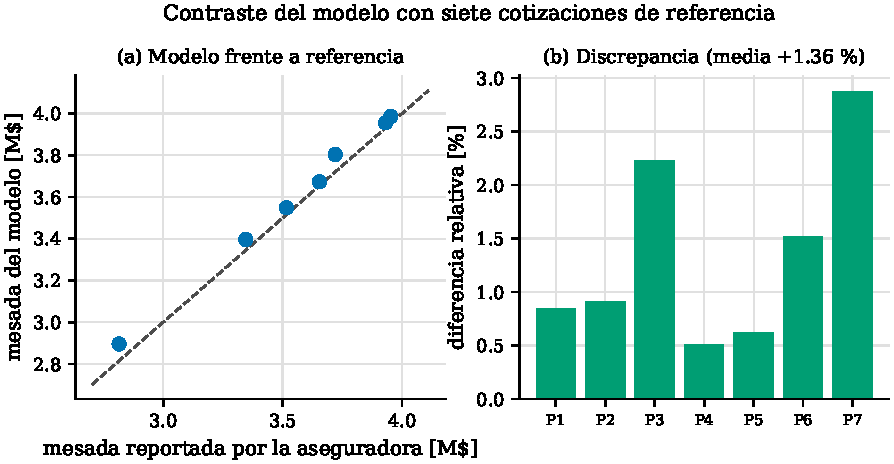
\includegraphics[width=\textwidth]{figuras/fig_validacion}
\caption[Contraste con cotizaciones reales]{Comparación del modelo con las
cotizaciones de referencia de la compañía para siete pólizas. La discrepancia media es de
$\datoValidMedia\%$, con un máximo de $\datoValidMax\%$.}
\label{fig:validacion}
\end{figure}

\section{Síntesis}

La revisión distingue datos normativos, hipótesis de valoración y convenciones del
cotizador. La procedencia de las series de mortalidad, los años base de mejora y
los ajustes de aplicabilidad requieren conciliación documental, y la volatilidad
de la cuenta individual, la calibración de Smith-Wilson y el factor NI limitan la
interpretación actuarial de las proyecciones. Para el análisis numérico, lo
esencial es que las modificaciones que solo alteran pesos independientes de $M$
conservan la representación afín a trozos de \cref{eq:canonica}; la posición de la
raíz y el desempeño de los métodos sí pueden cambiar, y la conservación de la forma
funcional no sustituye la validación de las bases actuariales.

\chapter{Extensión al retiro programado}
\label{cap:retiro}

El retiro programado es la modalidad alternativa a la renta vitalicia dentro del
régimen de ahorro individual: el pensionado conserva el saldo en su cuenta de
ahorro individual (CAI), administrada por la administradora de fondos de
pensiones, y retira cada año una mesada que se recalcula en función del saldo
remanente y de la expectativa de vida del grupo familiar. A diferencia de la renta
vitalicia, el riesgo de longevidad y el riesgo de mercado permanecen en cabeza del
pensionado\footnote{Artículo 81 de la Ley 100 de 1993. La modalidad se define allí como aquella en que el afiliado o los beneficiarios obtienen su pensión de la sociedad administradora con cargo a su cuenta individual y al bono pensional, calculándose cada año una anualidad en unidades de valor constante igual al resultado de dividir el saldo de la cuenta por el capital necesario para financiar una unidad de renta vitalicia para el afiliado y sus beneficiarios.}.
El mismo artículo contempla la protección del saldo necesario para financiar
una renta vitalicia mínima, con las excepciones previstas en su texto. El
cierre de una trayectoria computacional por insuficiencia de capital no
establece, por sí solo, la extinción del derecho pensional. Esta distinción
se mantiene al interpretar los experimentos de este capítulo.

Matemáticamente el cambio es sustancial: se pasa de \emph{un} problema de raíz a
\emph{una sucesión acoplada} de problemas de raíz sobre un sistema dinámico. Este
capítulo formaliza esa estructura y analiza la propagación del error a lo largo de
la recursión.

\section{Formulación}

\subsection{La recursión básica}

Sea $C_1=\KA$ el saldo inicial de la cuenta. Para fijar la indexación anual,
se escribe
\[
 \Phi_j^{\mathrm{RP}}=\Phi_j(\delta_{\mathrm{RP}}),\qquad j\ge0,
 \qquad S_0^{(n)}=S_0\Phi_{n-1}^{\mathrm{RP}},\qquad n\ge1,
\]
con el perfil de inflación de \cref{eq:factor-ipc}. El año $n=1$ es el de
valoración, por lo que $\Phi_0^{\mathrm{RP}}=1$ y $S_0^{(1)}=S_0$.
El deslizamiento $\delta_{\mathrm{RP}}$ es el parámetro alto de retiro
programado si la mesada reportada originalmente difiere del salario mínimo
en menos de un peso o si ese dato no está disponible; en los demás casos
es el parámetro bajo. Esta selección permanece fija durante la trayectoria.
Así, $S_0^{(n)}$ documenta el piso proyectado usado por el motor; la elección
de esa proyección no constituye por sí sola una validación normativa de sus
parámetros. Para $n\ge2$, el factor incremental es
\[
 r_n^{\mathrm{RP}}=
 \frac{\Phi_{n-1}^{\mathrm{RP}}}{\Phi_{n-2}^{\mathrm{RP}}}.
\]
El esquema siguiente describe
la recursión de valoración y balance del modelo implementado, cuyo alcance
se distingue de la operación normativa completa de la modalidad. Para cada
año $n=1,2,\dots$:

\begin{enumerate}[leftmargin=*]
  \item Se resuelve el problema de raíz del año $n$,
        \begin{equation}
        \label{eq:rp-raiz}
          \VP_n(M)\;=\;C_n ,
        \end{equation}
        donde $\VP_n$ es la función de valoración del \cref{cap:modelo}, evaluada
        con las edades del grupo familiar al año $n$ y con los parámetros propios
        del retiro programado: tabla de mortalidad sin factores de mejora,
        sobrecosto de mortalidad y recargo de gastos de retiro programado\footnote{Estas son convenciones del motor estudiado. Su uso en este experimento no demuestra que sean exigencias normativas ni sustituye la documentación de la base técnica aplicable; véase el \cref{cap:variables}.}. Sea
        $\widehat M_n$ su solución.
  \item Se aplican los operadores de ajuste regulatorio y comercial descritos en la
        \cref{sec:operadores}, obteniendo la mesada efectivamente pagada
        $M_n=\Psi_n(\widehat M_n,\,M_{n-1})$. Cuando se proporciona una
        trayectoria de referencia de renta vitalicia, la regla comercial del
        primer año fija $M_1=\max\{R_1,S_0^{(1)}\}$; no se interpreta esa
        igualdad como una conclusión del principio de equivalencia.
  \item Se actualiza el saldo:
        \begin{equation}
        \label{eq:rp-saldo}
          C_{n+1}\;=\;\bigl(C_n-\kappa\,M_n\bigr)\,(1+g_n),
        \end{equation}
        donde $\kappa\in\{13,14\}$ es el número de mesadas anuales. La tasa
        $g_n$ debe expresarse en la misma base monetaria que el saldo y los
        pagos. Este balance aproxima los retiros del año por un pago total
        anticipado, antes de aplicar el rendimiento anual.
  \item La simulación se interrumpe cuando el saldo no es positivo;
        el motor también se detiene si el solucionador declara que no
        convergió. Para identificar insuficiencia de capital para el mínimo
        proyectado, el criterio analítico es
        $C_n<\VP_n(S_0^{(n)})$. Esta desigualdad debe comprobarse mediante
        la valoración del mínimo y no queda acreditada por cualquier fallo
        numérico. El punto de interrupción es un diagnóstico del escenario,
        no una regla de terminación del derecho pensional.
\end{enumerate}

La coherencia monetaria requiere distinguir rendimientos reales y nominales.
Si los flujos y saldos están en pesos nominales y $g_n^{\mathrm{real}}$ es
el rendimiento real, la tasa nominal correspondiente satisface
\[
  1+g_n^{\mathrm{nominal}}
  =(1+g_n^{\mathrm{real}})(1+\pi_n).
\]
Si se trabaja en moneda constante, los pagos y el salario mínimo deben
deflactarse a una misma fecha base. La parametrización del motor denomina
real al rendimiento de la cuenta y presenta mesadas indexadas; su
conciliación monetaria y la aproximación anual de los pagos son limitaciones
de las trayectorias ilustradas, que no se presentan como una validación
financiera completa.

\begin{definition}[Sistema dinámico de retiro programado]
\label{def:sistema-rp}
El proceso anterior define el sistema dinámico
\begin{equation}
\label{eq:sistema}
  \begin{cases}
    M_n \;=\; \Psi_n\bigl(\VP_n^{-1}(C_n),\;M_{n-1}\bigr),\\[3pt]
    C_{n+1} \;=\; \bigl(C_n-\kappa M_n\bigr)(1+g_n),
  \end{cases}
  \qquad C_1=\KA .
\end{equation}
La regla de $\Psi_1$ incorpora el arranque comercial anterior cuando existe
una referencia $R_1$. Para los años siguientes el estado incluye la mesada
pagada el año anterior; $M_0$ es una referencia inicial común cuando se
necesita especificar ese argumento en el primer año.
\end{definition}

\begin{remark}[Qué tipo de objeto es esto]
La ecuación \cref{eq:sistema} define un sistema dinámico controlado sobre el estado
$(C_n,M_{n-1})$. La inversa corresponde a la mesada bruta sobre capitales
financiables. El solucionador anual mantiene el intervalo $[S_0,25S_0]$;
el piso proyectado $S_0^{(n)}$ se aplica a la mesada pagada y no reemplaza
automáticamente el extremo inferior de esa búsqueda. Cuando los rendimientos,
parámetros, referencias externas y reglas de activación se mantienen fijos,
la composición de inversas y recortes afines a trozos conserva esa estructura
en cada régimen admisible. Si se recalibran parámetros al cambiar el capital
o se activan reglas condicionales distintas, debe comprobarse de nuevo el
alcance de esta descripción y de las cotas de estabilidad.
\end{remark}

\subsection{Los operadores de ajuste}
\label{sec:operadores}

Además de la regla de arranque del primer año, se consideran cuatro ajustes
aplicados en el orden descrito. El piso del mínimo proyectado se distingue de las reglas
comerciales de presentación o de estabilización:

\begin{enumerate}[leftmargin=*]
  \item \textbf{Piso de crecimiento.}
        Para $n\ge2$, $M\mapsto\max\{M,M_{n-1}r_n^{\mathrm{RP}}\}$ cuando
        se activa la regla. En el motor, su activación exige que la mesada
        anterior y la bruta actual superen $S_0(1+10^{-9})$ y que el
        solucionador declare convergencia. Ese umbral de activación se
        distingue del mínimo proyectado $S_0^{(n)}$.
  \item \textbf{Piso del mínimo proyectado.}
        $M\mapsto\max\{M,S_0^{(n)}\}$.
  \item \textbf{Techo comercial (opcional).}
        $M\mapsto\min\{M,T_n\}$, donde
        $T_n=\max\{(1-\theta_n)R_n,S_0^{(n)}\}$ y $\theta_n$ es un margen
        creciente. El piso del mínimo tiene prioridad sobre el techo. Esta regla
        comercial está desactivada en la configuración por defecto y no
        demuestra una superioridad económica de la renta vitalicia.
  \item \textbf{Límite de caída.} $M\mapsto\max\{M,\;(1-\lambda)M_{n-1}\}$, con
        $\lambda=0{,}50$, que amortigua caídas interanuales. Se aplica después
        del techo y puede elevar de nuevo la mesada; por ello no se afirma
        que el orden final entre modalidades se cumpla para todo estado.
\end{enumerate}

\begin{proposition}[Propiedades del operador de ajuste]
\label{prop:psi}
Para una composición fija de los ajustes descritos, manteniendo constantes
la mesada anterior y las referencias externas, la aplicación
$M\mapsto\Psi_n(M,M_{n-1})$ es no decreciente, $1$-Lipschitz y afín a trozos.
Su derivada vale $1$ o $0$ en casi todo punto; una restricción estrictamente
activa anula la sensibilidad respecto de ese primer argumento. La regla
constante del primer año tiene las mismas propiedades.
\end{proposition}
\begin{proof}
Cada uno de los cuatro pasos es de la forma $M\mapsto\max\{M,\alpha\}$ o
$M\mapsto\min\{M,\beta\}$ con $\alpha,\beta$ independientes de $M$; ambas son no
decrecientes, $1$-Lipschitz y afines a trozos con pendiente $0$ o $1$
(\cref{lem:recorte}). La composición de aplicaciones no decrecientes y
$1$-Lipschitz lo es, y la clase afín a trozos es cerrada bajo composición
(\cref{lem:pl-cerrado}).
\end{proof}

\begin{criticism}[Sensibilidad de las mesadas ajustadas]
\label{crit:ajustes}
Una restricción activa puede anular la respuesta de la mesada pagada al
resultado bruto de valoración. Esto no elimina necesariamente su dependencia
del capital inicial: un piso construido con $M_{n-1}$ transmite la historia
de la trayectoria. Las salidas deben identificar la mesada bruta, la mesada
pagada y los ajustes aplicados. El experimento de la \cref{fig:propagacion}
ilustra un escenario de absorción de perturbaciones; no acredita que todos
los recortes eliminen el error en cualquier trayectoria.
\end{criticism}

\section{Propagación del error}
\label{sec:propagacion}

La pregunta práctica es: si el problema de raíz de cada año se resuelve con
tolerancia $\varepsilon$, ¿qué error arrastra la trayectoria completa? A diferencia
del caso de la renta vitalicia, donde el error se comete una sola vez, aquí se
acumula.

\begin{theorem}[Propagación del error en el estado acoplado]
\label{thm:propagacion}
Considérense una trayectoria exacta $(C_n,M_n)$ de \cref{eq:sistema}
y otra $(\widetilde C_n,\widetilde M_n)$ que emplea los mismos
rendimientos, funciones de valoración y parámetros de ajuste. El resultado
bruto del solucionador en la segunda trayectoria se denota por $U_n$ y
satisface
\[
  \left|U_n-\VP_n^{-1}(\widetilde C_n)\right|
  \le \varepsilon_n^x .
\]
Se supone que ambas trayectorias conservan soluciones admisibles hasta el
horizonte considerado y que, en un intervalo $I_n$ que contiene los valores
necesarios para la comparación,
\[
  |\VP_n(u)-\VP_n(v)|\ge m_n|u-v|,
  \qquad u,v\in I_n,\qquad m_n>0.
\]
Supóngase además que el operador de ajuste satisface
\[
  |\Psi_n(u,z)-\Psi_n(v,y)|
  \le |u-v|+L_n|z-y|,\qquad L_n\ge0,
\]
en el dominio considerado. Sean
$\delta_n=\widetilde C_n-C_n$ y
$\eta_n=\widetilde M_n-M_n$, donde
$\widetilde M_n=\Psi_n(U_n,\widetilde M_{n-1})$.
Entonces
\begin{equation}
\label{eq:prop-mesada}
  |\eta_n|\le \frac{|\delta_n|}{m_n}
       +L_n|\eta_{n-1}|+\varepsilon_n^x .
\end{equation}
Si las restantes operaciones del balance se consideran exactas,
\begin{equation}
\label{eq:prop-saldo}
  \delta_{n+1}=(1+g_n)(\delta_n-\kappa\eta_n).
\end{equation}
Defínanse
\[
  G_n=|1+g_n|,\qquad a_n=\frac{\kappa}{m_n},\qquad
  E_n=\begin{pmatrix}|\delta_n|\\ \kappa|\eta_{n-1}|\end{pmatrix},
  \qquad
  A_n=\begin{pmatrix}
       G_n(1+a_n)&G_nL_n\\
       a_n&L_n
      \end{pmatrix}.
\]
La siguiente desigualdad se interpreta componente a componente:
\begin{equation}
\label{eq:prop-cota}
  E_{n+1}\le A_nE_n+
       \kappa\varepsilon_n^x
       \begin{pmatrix}G_n\\1\end{pmatrix}.
\end{equation}
Escribiendo $\mathcal P_{r:s}=A_rA_{r-1}\cdots A_s$ para $r\ge s$ y
$\mathcal P_{r:s}=I$ para $r<s$, resulta
\[
 E_{N+1}\le \mathcal P_{N:1}E_1+
 \sum_{j=1}^{N}\mathcal P_{N:j+1}
       \kappa\varepsilon_j^x
       \begin{pmatrix}G_j\\1\end{pmatrix}.
\]
\end{theorem}
\begin{proof}
La condición de crecimiento de $\VP_n$ implica que su inversa es
$1/m_n$-Lipschitz en el intervalo correspondiente de capitales. Por la
desigualdad triangular,
\[
 |U_n-\VP_n^{-1}(C_n)|
 \le\varepsilon_n^x+\frac{|\delta_n|}{m_n}.
\]
Al aplicar la hipótesis sobre $\Psi_n$ se obtiene
\cref{eq:prop-mesada}. La resta de los balances da
\cref{eq:prop-saldo}; por tanto,
\[
 |\delta_{n+1}|\le G_n\bigl(|\delta_n|+\kappa|\eta_n|\bigr).
\]
Al sustituir la cota de la mesada se obtiene la primera fila de
\cref{eq:prop-cota}; la segunda resulta de multiplicar
\cref{eq:prop-mesada} por $\kappa$. Todas las entradas de $A_n$ son no
negativas, de modo que la desigualdad puede iterarse.
\end{proof}

\begin{remark}[Alcance de las hipótesis]
La $1$-Lipschitzianidad de la \cref{prop:psi} se refiere al primer
argumento de $\Psi_n$, con la mesada anterior fija. El término
$L_n|\eta_{n-1}|$ incorpora la perturbación del segundo argumento.
Para la composición fija de los recortes descritos, con referencias
externas comunes, una cota de esa dependencia es
$L_n=\max\{r_n^{\mathrm{RP}},1-\lambda\}$ para $n\ge2$; en el
arranque constante puede tomarse $L_1=0$. Si la regla de crecimiento
permanece inactiva, basta $L_n=1-\lambda$.
La selección condicional de la regla de crecimiento no es una composición
fija de recortes: al cruzar su umbral puede introducir un salto si el piso
histórico es superior a las dos mesadas brutas. Por ello la
\cref{prop:psi} y la cota matricial no acreditan una propiedad de
Lipschitz global del programa. Al comparar estados con activaciones
distintas debe verificarse expresamente la desigualdad exigida por el
teorema; sin ella no se aplica esa cota.

El resultado se aplica hasta el horizonte común de admisibilidad y no
acota por sí solo la diferencia entre los años de interrupción de dos
proyecciones. Tampoco incluye cambios de las referencias de renta vitalicia,
de la calibración del factor NI o de los rendimientos entre trayectorias.
Si esos elementos dependen del capital perturbado, debe incorporarse
su variación como un término adicional.
\end{remark}

\begin{corollary}[Regímenes locales]
\label{cor:regimenes}
Sin error local del solucionador, los siguientes son regímenes particulares:
\begin{enumerate}[label=(\roman*),leftmargin=*]
  \item Si ninguna restricción modifica la mesada bruta en las dos
        trayectorias y $\VP_n(M)=s_nM+b_n$ en su tramo común, con
        $s_n>0$, entonces
        \[
          \eta_n=\frac{\delta_n}{s_n},\qquad
          \delta_{n+1}=(1+g_n)
          \left(1-\frac{\kappa}{s_n}\right)\delta_n.
        \]
        Hay contracción del error del saldo cuando
        $|(1+g_n)(1-\kappa/s_n)|<1$.
  \item Si el ajuste fija la misma mesada externa en ambas trayectorias,
        independientemente de la mesada anterior, entonces
        $\eta_n=0$ y $\delta_{n+1}=(1+g_n)\delta_n$.
  \item Si está activo un piso dependiente de la mesada anterior, con
        $\Psi_n(u,z)=r_nz$ en el régimen común, entonces
        $\eta_n=r_n\eta_{n-1}$. La anulación de la derivada respecto de
        $u$ no elimina la perturbación transmitida por la historia.
\end{enumerate}
\end{corollary}

\begin{figure}[H]
\centering
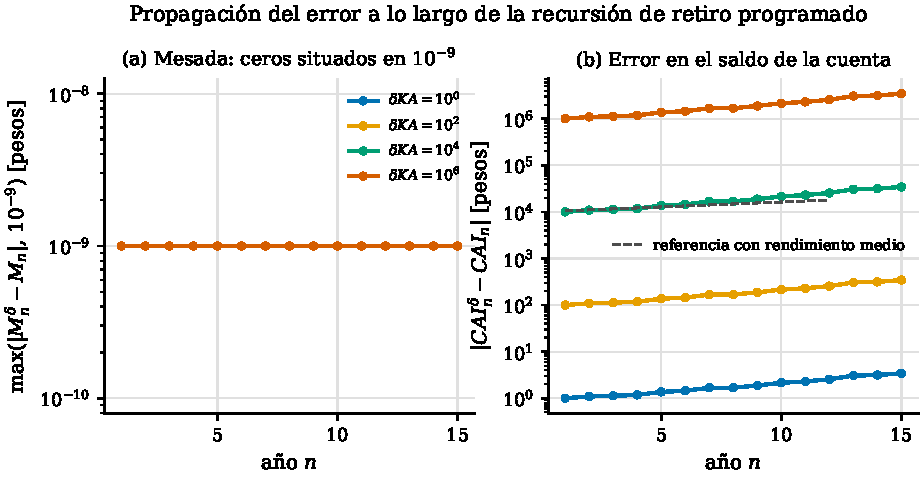
\includegraphics[width=\textwidth]{figuras/fig_propagacion_error_rp}
\caption[Propagación del error en retiro programado]{Experimento ilustrativo
con perturbaciones del capital inicial de $10^0$, $10^2$, $10^4$ y $10^6$
pesos, utilizando los mismos rendimientos en las trayectorias comparadas.
El panel (a) muestra las diferencias de mesada del escenario y el panel (b),
las diferencias de saldo. La línea discontinua es una referencia geométrica
construida con el rendimiento medio; no constituye una cota general cuando
los rendimientos varían. La absorción de perturbaciones depende del régimen
activo y de su dependencia de la mesada anterior (\cref{cor:regimenes}).}
\label{fig:propagacion}
\end{figure}

\begin{corollary}[Tolerancia admisible según el horizonte]
\label{cor:tolerancia-rp}
Bajo las hipótesis del \cref{thm:propagacion}, supóngase que el estado inicial
es el mismo en ambas trayectorias, $E_1=0$, y que
$\varepsilon_n^x\le\varepsilon_x$. Sea $e_1=(1,0)^{\mathsf T}$ y defínase
\[
 H_N^x=e_1^{\mathsf T}
 \sum_{j=1}^{N}\mathcal P_{N:j+1}
       \kappa\begin{pmatrix}G_j\\1\end{pmatrix}.
\]
Entonces $|\delta_{N+1}|\le H_N^x\varepsilon_x$. Si $H_N^x>0$, la condición
suficiente
\[
  \varepsilon_x\le\frac{\Delta}{H_N^x}
\]
garantiza un error del saldo final no mayor que $\Delta$.

Si la tolerancia anual se expresa en unidades de residuo,
$|\VP_n(U_n)-\widetilde C_n|\le\varepsilon_f$, y $U_n\in I_n$,
puede utilizarse $\varepsilon_n^x\le\varepsilon_f/m_n$. En ese caso basta
\[
 \varepsilon_f\le\frac{\Delta}{H_N^f},\qquad
 H_N^f=e_1^{\mathsf T}
 \sum_{j=1}^{N}\mathcal P_{N:j+1}
       \frac{\kappa}{m_j}\begin{pmatrix}G_j\\1\end{pmatrix},
\]
siempre que $H_N^f>0$.
\end{corollary}
\begin{proof}
Se toma la primera componente de la cota iterada del
\cref{thm:propagacion} y se utilizan, respectivamente,
$\varepsilon_j^x\le\varepsilon_x$ y
$\varepsilon_j^x\le\varepsilon_f/m_j$.
\end{proof}

El corolario distingue la tolerancia del residuo, medida en unidades de
capital, de la tolerancia de mesada. Su elección depende del horizonte,
las pendientes y la dependencia temporal de los ajustes. No se deduce un
factor universal de endurecimiento a partir del rendimiento medio y del
número de años solamente. La recomendación~R4 de la
\cref{sec:hallazgos-codigo} consiste en calibrar y verificar la tolerancia
para la configuración concreta de la proyección.

\section{El costo computacional del acoplamiento}

Una trayectoria de $N$ años requiere resolver hasta $N$ problemas de raíz.
Su costo es la suma de las llamadas efectivas al motor en esos años, incluyendo
la preparación de los datos y las derivadas. El promedio del banco de
cotizaciones de renta vitalicia no constituye por sí solo una medición del
costo de esta recursión: cambian las edades, las reservas financiables y
los ajustes activos. Las cifras de una trayectoria completa deben medirse
sobre esa trayectoria.

\begin{remark}[Arranque en caliente]
La mesada del año anterior puede utilizarse como punto inicial de la
valoración siguiente, expresada en la misma base monetaria. Si ese arranque
y la nueva raíz pertenecen al interior de un mismo tramo afín, el
apartado (i) del \cref{thm:terminacion-finita} garantiza que una propuesta de Newton con su pendiente
exacta alcanza la raíz; si se aplica una salvaguarda, debe verificarse además
que dicha propuesta se acepte. La proximidad de dos mesadas no demuestra
por sí sola esta condición, pues también cambia la función de valoración.
La ganancia del arranque en caliente requiere una medición específica y
no se le asigna un factor universal de aceleración.
\end{remark}

\section{Comparación entre las dos modalidades}

\begin{figure}[H]
\centering
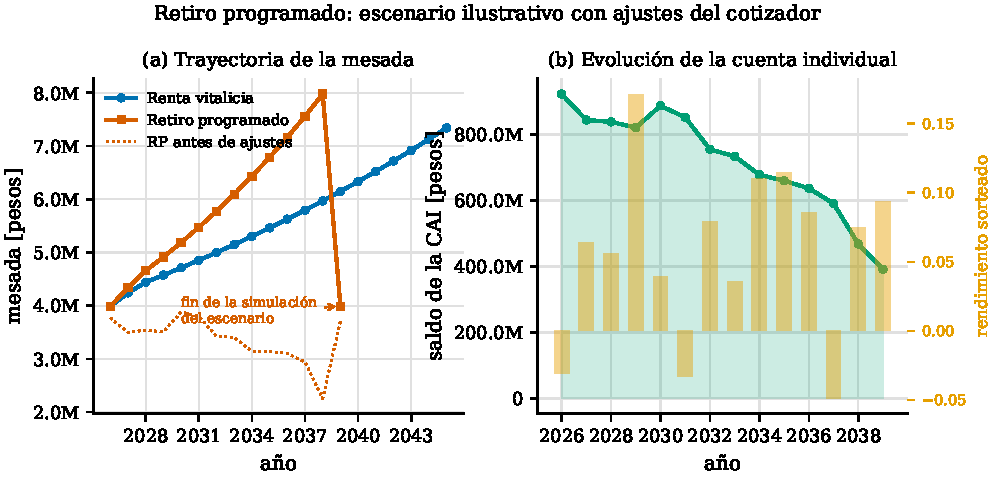
\includegraphics[width=\textwidth]{figuras/fig_rp_vs_rv}
\caption[Renta vitalicia frente a retiro programado]{Escenario ilustrativo
para una póliza. Panel (a): mesadas proyectadas bajo las hipótesis y reglas
del motor; la línea punteada muestra la mesada bruta de retiro programado
antes de los ajustes. El punto donde termina una serie indica la
interrupción de la simulación y no la extinción del derecho pensional.
Panel (b): evolución del saldo y rendimientos anuales sorteados. Una
trayectoria no establece una comparación general de los riesgos ni una
superioridad económica entre modalidades.}
\label{fig:rp-vs-rv}
\end{figure}

Las modalidades distribuyen de forma diferente los riesgos del pensionado y
de las entidades participantes. El escenario de la figura está condicionado
por los parámetros financieros, las reglas comerciales y los rendimientos
sorteados; en particular, el arranque puede estar fijado a la misma mesada
de renta vitalicia. Para comparar riesgos harían falta conjuntos de
trayectorias, hipótesis contrastadas y medidas de su distribución.

Desde el punto de vista numérico, las valoraciones anuales de retiro
programado pertenecen a la misma familia de máximos y recortes que la renta
vitalicia cuando sus coeficientes no dependen de la mesada buscada. No son
la misma función: los parámetros, las edades y los recargos pueden variar.
La estructura afín a trozos permite aprovechar derivadas laterales exactas
en cada problema, mientras que el acoplamiento temporal exige el control
del estado y de los errores locales establecido en este capítulo.

\chapter{Experimentos numéricos}
\label{cap:resultados}

Este capítulo contrasta los \crefrange{cap:estructura}{cap:metodos} con
\datoNMetodos{} métodos sobre \datoNEscenarios{} escenarios del motor estudiado.

\section{Diseño experimental}
\subsection{Los escenarios}
Se distinguen \datoNSinteticos{} escenarios sintéticos, \datoNReales{}
cotizaciones RV y \datoNRealesRP{} registros adicionales que incluyen datos de RP.

\paragraph{Escenarios sintéticos.}
Se seleccionan combinaciones de perfiles demográficos y regiones objetivo;
los nueve casos no constituyen el producto cartesiano de todos los perfiles
con todas las regiones. Se incluyen causantes de distinta edad, sexo y
condición de invalidez, con y sin beneficiarios.
\begin{center}
\small
\begin{tabular}{@{}llp{7.2cm}@{}}
\toprule
\textbf{Código} & \textbf{Objetivo} & \textbf{Región estructural} \\
\midrule
\texttt{R2} & $1{,}037\,S_0$ & racimo I: piso del salario mínimo \\
\texttt{R3} & $2{,}414\,S_0$ & tramo afín comercial \\
\texttt{R4} & $5{,}236\,S_0$ & racimo II: activación del auxilio funerario \\
\texttt{R5} & $10{,}372\,S_0$ & racimo III: saturación del auxilio funerario \\
\bottomrule
\end{tabular}
\end{center}
Para cada caso se fija una mesada objetivo y se toma
$\KA=\VP(M_{\mathrm{objetivo}})$. La solución es conocida por construcción,
hasta el redondeo de la evaluación del capital.
\begin{remark}[Elección de los objetivos]
Los objetivos se construyen a partir de constantes irracionales, representadas
en punto flotante. Esto reduce la coincidencia deliberada con los puntos
medios del encaje (\cref{rem:sesgo-diadico}); no elimina el redondeo ni
prueba ausencia de sesgo para toda implementación.
\end{remark}

\paragraph{Cotizaciones reales.}
Los capitales proceden de los archivos de cotización. Las referencias
numéricas obtenidas con Brent a tolerancia estricta se contrastan con una
implementación independiente de SciPy. Se reporta diferencia respecto de
una referencia numérica, no de una solución exacta conocida. La concordancia
con las mesadas de la compañía se analiza aparte en la \cref{sec:validacion}.
Los siete registros adicionales se valoran en este banco con la función
RV: su procedencia no significa que los \datoNMetodos{} métodos se hayan
comparado sobre las recursiones anuales completas de RP.
La financiación exactamente mínima y la insuficiencia se estudian mediante
el \cref{thm:existencia} y comprobaciones específicas; no son casos con
raíz interior incluidos en los porcentajes ordinarios de éxito.

\subsection{Protocolo}
\begin{itemize}[leftmargin=*,nosep]
\item Encaje $[S_0,25S_0]$. El extremo superior es una decisión de búsqueda,
      no un límite contractual general.
\item Arranque abierto: punto medio; secante: extremos; Müller: extremos y punto medio.
\item Tolerancias $\varepsilon_f=\datoEpsilonProd$ peso de capital y
      $\varepsilon_x=10^{-8}$ pesos de mesada, según \cref{eq:parada}.
      El paso pequeño no certifica éxito por sí solo.
\item Diferencias centradas con $h=1$ peso de mesada.
\item Costo: llamadas efectivas al motor, incluidas derivadas y preparación,
      con memoria independiente por método y ejecución.
\end{itemize}
Newton analítico y semisuave calculan conjuntamente valor y derivadas por punto.
Punto fijo, Aitken y Steffensen escalado incluyen la derivada inicial que prepara
la relajación. No se comparte memoria entre métodos ni repeticiones.
Se realizan tres repeticiones de producción; el tiempo por caso es su mediana,
y los promedios por método se calculan después sobre los casos.
Una batería adicional utiliza $\varepsilon_f=10^{-6}$ y $\varepsilon_x=10^{-10}$.
Los tiempos describen el entorno registrado y no garantizan rendimiento en otra máquina.

\section{Resultados globales}
\begin{table}[H]
\centering
\caption[Resultados globales de la comparación]{Comparación sobre
\datoNEscenarios{} escenarios, ordenada por llamadas al motor. «Éxito» indica
cumplimiento del criterio certificado; «Ev.» incluye valor, derivadas y preparación.
El error es la mediana de las diferencias absolutas de mesada respecto de la
referencia. El costo de una ejecución fallida no representa el de una solución.}
\label{tab:resultados-globales}
\small
\begin{tabular}{@{}llrrrrr@{}}
\toprule
\textbf{Método} & \textbf{Familia} & \textbf{Éxito} & \textbf{Ev.\ media} & \textbf{Ev.\ máx.} & \textbf{Iter.} & \textbf{Error mediano} \\
\midrule
Steffensen & abierto & 0\% & 3{,}00 & 3 & 1{,}00 & $1{,}8\cdot10^{6}$ \\
Newton (analítico) & abierto & 100\% & 3{,}08 & 5 & 2{,}08 & $4{,}7\cdot10^{-10}$ \\
Newton semisuave & no suave & 100\% & 3{,}08 & 5 & 2{,}08 & $4{,}7\cdot10^{-10}$ \\
Punto fijo relajado & abierto & 100\% & 3{,}48 & 9 & 2{,}48 & $9{,}3\cdot10^{-10}$ \\
Aitken--Steffensen & abierto & 100\% & 4{,}32 & 5 & 1{,}84 & $0$ \\
Secante & abierto & 100\% & 5{,}08 & 8 & 4{,}08 & $4{,}7\cdot10^{-10}$ \\
Anderson--Björck & encaje & 100\% & 5{,}08 & 8 & 3{,}08 & $3{,}7\cdot10^{-6}$ \\
Pegasus & encaje & 100\% & 5{,}08 & 8 & 3{,}08 & $6{,}6\cdot10^{-6}$ \\
Steffensen escalado & abierto & 100\% & 5{,}24 & 11 & 2{,}12 & $9{,}3\cdot10^{-10}$ \\
Brent & encaje & 100\% & 5{,}28 & 9 & 3{,}28 & $0$ \\
Newton salvaguardado & no suave & 100\% & 5{,}52 & 11 & 2{,}52 & $4{,}7\cdot10^{-10}$ \\
Illinois & encaje & 100\% & 5{,}80 & 9 & 3{,}80 & $4{,}7\cdot10^{-10}$ \\
Regula falsi & encaje & 100\% & 5{,}80 & 11 & 3{,}80 & $3{,}9\cdot10^{-6}$ \\
Müller & abierto & 100\% & 6{,}08 & 9 & 5{,}08 & $1{,}1\cdot10^{-5}$ \\
Newton (dif.\ finitas) & abierto & 100\% & 7{,}60 & 13 & 2{,}20 & $2{,}3\cdot10^{-6}$ \\
Ridders & encaje & 100\% & 9{,}84 & 20 & 3{,}92 & $4{,}7\cdot10^{-10}$ \\
Halley & abierto & 100\% & 10{,}16 & 17 & 3{,}08 & $8{,}4\cdot10^{-6}$ \\
ITP & encaje & 100\% & 29{,}64 & 30 & 27{,}64 & $1{,}1\cdot10^{-3}$ \\
Bisección & encaje & 100\% & 33{,}40 & 35 & 31{,}40 & $1{,}6\cdot10^{-3}$ \\
\bottomrule
\end{tabular}
\end{table}
Newton analítico y semisuave requieren $\datoEvNAN$ llamadas medias.
Con la derivada lateral derecha seleccionada, sus iteraciones coinciden en
esta muestra. Bisección requiere $\datoEvBis$ y Newton con diferencias
finitas, $\datoEvNFD$. La razón de llamadas entre bisección y Newton analítico
es $\datoAceleracionNewton$; la reducción frente a diferencias finitas es
$\datoAhorroDerivada\%$. Estas cifras corresponden al cálculo conjunto verificado;
una implementación con dos llamadas separadas debe contabilizar ambas.
Secante requiere $\datoEvSec$ llamadas y punto fijo, $\datoEvPF$, incluida
la preparación. Halley emplea $\datoEvHal$, sin ventaja frente a Newton en
estos casos. Steffensen sin escalado falla en la batería con los recortes y
la escala empleados (\cref{crit:steffensen}).
\begin{figure}[H]
\centering
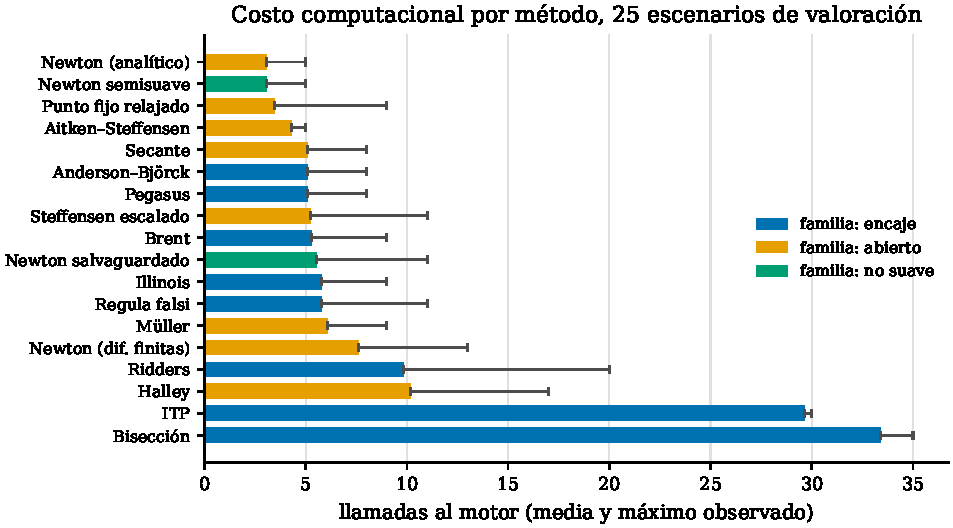
\includegraphics[width=.92\textwidth]{figuras/fig_barras_evaluaciones}
\caption[Costo computacional por método]{Llamadas al motor: media y segmento
hasta el máximo observado. El máximo describe la muestra y no constituye
una cota para una cartera arbitraria.}
\label{fig:barras}
\end{figure}

\section{Alcance de la estimación del orden}
\begin{figure}[H]
\centering
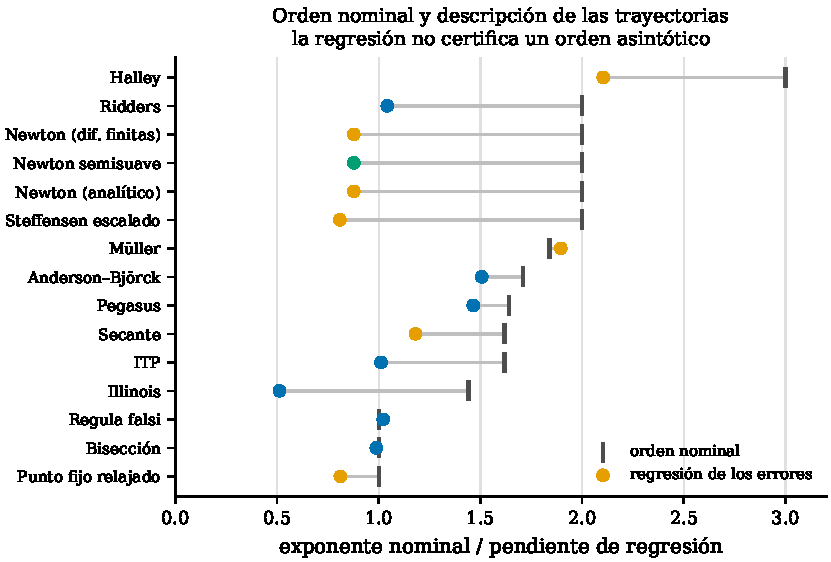
\includegraphics[width=.72\textwidth]{figuras/fig_orden_empirico}
\caption[Orden nominal y estimación por regresión]{Orden nominal y pendiente
estimada por regresión cuando hay suficientes errores útiles. Se omiten los
casos sin estimación o sin orden nominal fijo. Los valores no certifican
por sí solos el orden asintótico.}
\label{fig:orden}
\end{figure}
El orden clásico requiere regularidad y un régimen asintótico. Al cruzar
quiebres pueden faltar esas hipótesis; al alcanzar un tramo afín puede ocurrir
terminación exacta en aritmética ideal. En el segundo caso quedan muy pocos
errores antes del redondeo y el orden no es estimable de forma fiable.
Una regresión sobre iteraciones transitorias no demuestra pérdida del orden
teórico. Se comparan principalmente éxito, residuo, llamadas y tiempo.

\section{Resultados por región estructural}
\label{sec:res-por-region}
\begin{table}[H]
\centering
\caption[Costo por región estructural]{Llamadas medias al motor por región
que contiene la raíz de los escenarios sintéticos.}
\label{tab:por-region}
\small
\begin{tabular}{@{}lrrrr@{}}
\toprule
\textbf{Método} & \textbf{R2 (racimo I)} & \textbf{R3 (afín)} & \textbf{R4 (racimo II)} & \textbf{R5 (racimo III)} \\
\midrule
Bisección & 33{,}0 & 34{,}0 & 34{,}0 & 33{,}0 \\
Brent & 8{,}5 & 5{,}0 & 5{,}0 & 5{,}0 \\
Illinois & 9{,}0 & 6{,}0 & 5{,}0 & 5{,}0 \\
Secante & 8{,}0 & 5{,}0 & 5{,}0 & 5{,}0 \\
Newton (dif.\ finitas) & 13{,}0 & 7{,}0 & 10{,}0 & 7{,}0 \\
Newton (analítico) & 5{,}0 & 3{,}0 & 4{,}0 & 3{,}0 \\
Newton salvaguardado & 10{,}5 & 5{,}0 & 8{,}0 & 5{,}0 \\
Punto fijo relajado & 8{,}5 & 3{,}0 & 5{,}0 & 4{,}0 \\
Halley & 13{,}0 & 10{,}0 & 10{,}0 & 7{,}0 \\
\bottomrule
\end{tabular}
\end{table}
En R3, el paso de Newton obtiene la raíz cuando selecciona la pendiente del
tramo que la contiene (\cref{cor:un-paso}); el resultado no limita a un paso
los arranques exteriores. En R2 la pendiente próxima al mínimo es menor y
cambia al activarse nuevos periodos. En R4 y R5 el cambio del auxilio es pequeño
para las bases examinadas, aunque afecta las garantías basadas en convexidad.
\begin{figure}[H]
\centering
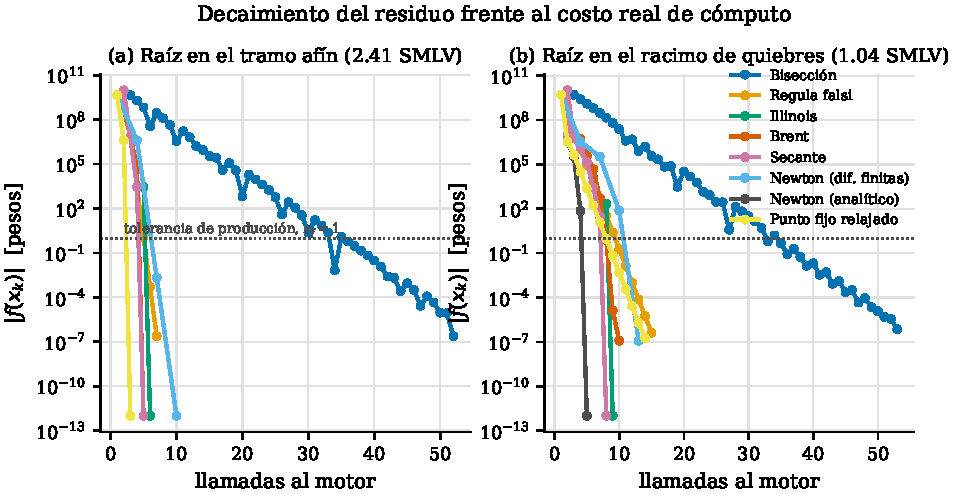
\includegraphics[width=\textwidth]{figuras/fig_convergencia_residuos}
\caption[Decaimiento del residuo]{Residuo de valoración frente a llamadas
acumuladas al motor, en escala logarítmica. La línea horizontal indica un
peso de capital; los paneles corresponden al tramo afín y al racimo I.}
\label{fig:residuos}
\end{figure}
\begin{figure}[H]
\centering
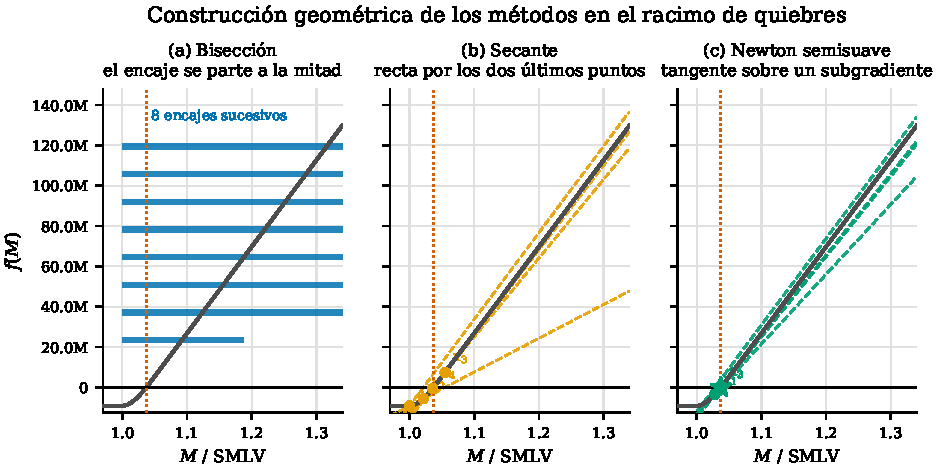
\includegraphics[width=\textwidth]{figuras/fig_trayectorias}
\caption[Construcción geométrica de los métodos]{Construcción de bisección,
secante y Newton semisuave cerca del racimo I. La ampliación muestra cambios
de pendiente y no sustituye las hipótesis de los teoremas.}
\label{fig:trayectorias}
\end{figure}

\section{Robustez frente al punto inicial}
\label{sec:robustez-empirica}
\begin{figure}[H]
\centering
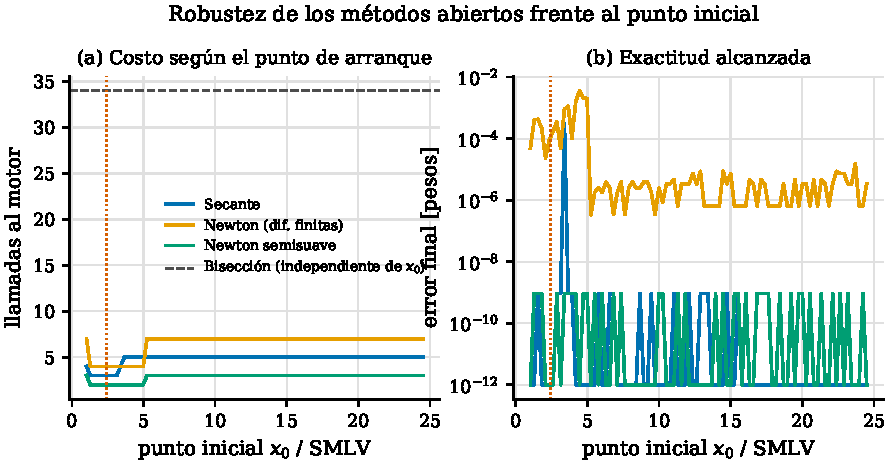
\includegraphics[width=\textwidth]{figuras/fig_robustez_inicial}
\caption[Robustez frente al punto inicial]{Costo y error final para A-R3,
en una malla de 90 arranques entre $1{,}02S_0$ y $24{,}5S_0$.
Cada ejecución dispone de memoria propia y se comprueba el residuo.}
\label{fig:robustez}
\end{figure}
El barrido describe un escenario y una malla finita. Los métodos con encaje,
incluidos la variante salvaguardada y Brent, parten del intervalo inicial y no
de $x_0$; por eso solo la bisección figura en el barrido, como referencia.
La convergencia monótona
del \cref{thm:terminacion-finita}(ii) requiere convexidad en el intervalo
recorrido y arranque a la derecha. La variante salvaguardada dispone de la
garantía del \cref{thm:salvaguardado}; Brent y otros métodos con encaje también
ofrecen garantías bajo sus condiciones. El barrido no demuestra robustez global
de los métodos abiertos para cualquier póliza.

\section{Costo frente a precisión exigida}
\begin{figure}[H]
\centering
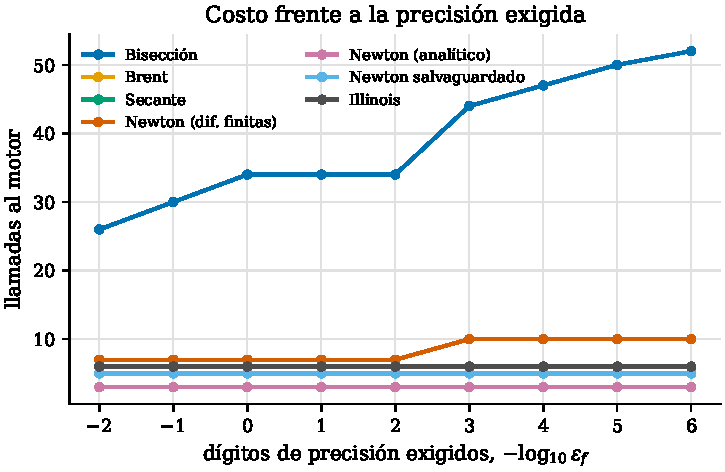
\includegraphics[width=.78\textwidth]{figuras/fig_costo_tolerancia}
\caption[Costo frente a precisión]{Llamadas al motor frente a tolerancia de
residuo en A-R3. El costo casi constante de algunos métodos corresponde a
este escenario y al rango de tolerancias representado.}
\label{fig:costo-tolerancia}
\end{figure}
La cota de bisección aumenta aproximadamente $\log_2(10)$ pasos por dígito
decimal adicional de exactitud en la variable. En un tramo afín, Newton con
pendiente exacta puede alcanzar el redondeo sin iteraciones adicionales al
endurecer la tolerancia. Una tolerancia inferior al residuo alcanzable en punto
flotante no implica convergencia ni exactitud adicional.

\section{Contraste sobre cotizaciones reales}
Las soluciones de los dos conjuntos reales se sitúan entre $\datoMultMin$ y
$\datoMultMax$ salarios mínimos, con media $\datoMultMedia$. En esta muestra
quedan en el tramo afín $[\datoAnchoRacimo,5]S_0$. Esto explica la utilidad de
la pendiente exacta; no prueba que toda la cartera o todo el mercado tenga
esa propiedad ni valida las bases actuariales. El contraste de la
\cref{sec:validacion} requiere conciliar datos, hipótesis y recargos.

\section{Hallazgos sobre la implementación de producción}
\label{sec:hallazgos-codigo}
Se distingue la corrección del banco de su adopción en todos los flujos de producción.
\begin{table}[H]
\centering
\caption[Recomendaciones sobre la implementación]{Correcciones y recomendaciones.
La verificación del catálogo no certifica todos los recorridos de la aplicación.}
\label{tab:hallazgos}
\small
\begin{tabular}{@{}>{\raggedright\arraybackslash}p{.55cm}>{\raggedright\arraybackslash}p{4.1cm}>{\raggedright\arraybackslash}p{5.2cm}>{\raggedright\arraybackslash}p{3.1cm}@{}}
\toprule
& \textbf{Acción} & \textbf{Fundamento} & \textbf{Estado} \\
\midrule
R1 & Distinguir insuficiencia de fallo numérico. & $\KA<\VP(S_0)$ identifica
insuficiencia; el fracaso del método no la demuestra. & Comprobado en sensibilidad;
integración general pendiente. \\
\midrule
R2 & Corregir la derivada en $M=S_0$. & \cref{prop:continuidad-rama}: la rama
altera la fórmula de la derivada aunque conserve el valor. & Implementado en el motor. \\
\midrule
R3 & Certificar el error y declarar sus unidades. & $|x-M^*|\le |f(x)|/m$
requiere cota inferior válida; el ancho del encaje ofrece otro certificado. &
Criterio corregido en el banco. \\
\midrule
R4 & Elegir la tolerancia anual de RP según horizonte. & \cref{cor:tolerancia-rp}:
intervienen el estado acoplado, rendimientos y errores locales. & Cota formulada;
calibración operativa pendiente. \\
\midrule
--- & Calcular conjuntamente valor y derivada. & Una llamada por punto;
ahorro observado de $\datoAhorroDerivada\%$ frente a diferencias finitas. &
Implementado y contado en el banco. \\
\bottomrule
\end{tabular}
\end{table}

\section{Recomendación}
\begin{aporte}
Para el modelo estudiado, cuando se dispone de la derivada analítica, se recomienda
Newton semisuave con salvaguarda periódica (\cref{alg:newton-salvaguardado}).
Combina la reducción cuantitativa del encaje con la terminación local afín a
trozos. En la batería completa emplea $\datoEvNSG$ llamadas medias, frente a
$\datoEvBis$ de bisección, $\datoEvSec$ de secante y $\datoEvBre$ de Brent.

La comparación con Brent depende de la región de la raíz. En las cotizaciones
reales, situadas en el tramo afín, el salvaguardado requiere $4{,}78$ y
$4{,}71$ llamadas medias en los dos conjuntos, frente a $5{,}00$ de Brent; las
dos llamadas adicionales respecto de Newton semisuave sin salvaguarda
corresponden a la evaluación de los extremos del encaje. En los escenarios
sintéticos, que sitúan deliberadamente raíces en los racimos de quiebres,
requiere $6{,}89$ frente a $5{,}78$ de Brent (\cref{tab:por-region}).

La preferencia por el salvaguardado no descansa, por tanto, en un menor costo
en todos los casos. Se apoya en que aprovecha la pendiente exacta para obtener
la raíz por inversión del tramo que la contiene, en que su paso tiene una
lectura actuarial directa (\cref{thm:subdiferencial}) y en la cota global del
\cref{thm:salvaguardado}, que no es la misma cota por iteración de la bisección
pura. Cuando no se dispone de derivadas, Brent ofrece una alternativa con encaje
y costo similar. La secante es competitiva en costo, pero su versión abierta
carece de esa garantía global. La elección operativa requiere verificar dominio,
bases actuariales y certificados de salida.
\end{aporte}

\chapter{Conclusiones}
\label{cap:conclusiones}

\section{Respuesta a la pregunta de investigación}

La elección del método se sustenta en la estructura del cotizador y en el costo de
su implementación. La caracterización analítica obtenida puede resumirse así:

\begin{aporte}
En el modelo estudiado, la valoración es \textbf{afín a trozos}, con umbrales
candidatos organizados en tres racimos geométricos para la parametrización
considerada. La extensión a $M\ge0$ es constante en $[0,\SMLV]$, mientras que en
el dominio admisible $M\ge\SMLV$ hay una raíz única si y solo si
$\KA\ge\VP(\SMLV)$. El auxilio funerario puede destruir la convexidad. Las
mesadas de la muestra de renta vitalicia examinada se sitúan en un intervalo
afín; esa observación no describe la cartera completa de la compañía ni el
mercado colombiano.
\end{aporte}

La derivada lateral exacta permite aprovechar los tramos sin aproximar pendientes
por valoraciones auxiliares. Un paso de Newton obtiene la raíz cuando la clausura
del tramo seleccionado contiene también la solución. Esta propiedad no garantiza
una o dos iteraciones desde todo arranque ni identifica los pasos con el número
de tramos atravesados. Para el problema interior con un encaje inicial válido, la
variante semisuave con bisección periódica aporta una garantía global explícita
(\cref{thm:salvaguardado}), por lo que constituye una recomendación fundada para
el cotizador estudiado. Su costo y el de las otras alternativas deben leerse en
el \cref{cap:resultados}, con la contabilidad completa allí definida; la
recomendación no establece una superioridad universal.

\section{Verificación de las hipótesis de trabajo}

\begin{description}[leftmargin=1.1cm,style=nextline]
\item[H1 --- caracterización analítica.] La representación afín a trozos y el
  conjunto de hasta $\datoNQuiebresMax$ umbrales candidatos se obtienen de las
  operaciones de máximo y recorte (\cref{thm:quiebres}). Un umbral candidato
  puede no producir un salto efectivo si su peso es nulo.

\item[H2 --- terminación bajo condiciones precisas.] La inversión exacta de un
  tramo da la terminación en un paso si este contiene la raíz en su clausura.
  La cota por número de tramos requiere las condiciones adicionales del
  \cref{thm:terminacion-finita}; no es una igualdad general. Los experimentos
  ilustran estas condiciones, sin convertir el comportamiento de la muestra en
  una garantía para toda cotización.

\item[H3 --- contabilidad de costo.] Las iteraciones no representan el mismo
  trabajo en todos los métodos. La comparación contabiliza preparación,
  valoraciones auxiliares y llamadas efectivas al motor, y las complementa con
  tiempo de ejecución. Los cocientes de costo corresponden al protocolo y al
  entorno medidos.

\item[H4 --- derivada analítica conjunta.] Reutilizar los vectores de valoración
  evita las llamadas auxiliares de las diferencias finitas. El costo marginal de
  las derivadas no se considera nulo, y el ahorro efectivo se evalúa con el oráculo
  conjunto de valor y derivadas. No se deduce un porcentaje fijo del número
  nominal de evaluaciones por iteración.
\end{description}

\section{Contribuciones}

\subsection{Al análisis del problema}

El aporte central es integrar herramientas conocidas de valoración y análisis no
suave para estudiar este cotizador. La condición de capital mínimo distingue
falta de financiación, solución en el piso y solución interior. La expresión de
las derivadas laterales da acceso al $B$-subdiferencial y relaciona el error de
reserva con el de mesada. Las condiciones de terminación y el encaje separan la
rapidez local de la garantía global.

En retiro programado, el estado incluye el saldo y la mesada anterior porque los
ajustes dependen de ambos. La cota del \cref{thm:propagacion} incorpora ese
acoplamiento y permite escoger tolerancias a partir de un error admisible del
saldo final, bajo sus hipótesis. No implica una amplificación universal ni
permite comparar la conveniencia de las modalidades pensionales.

\subsection{A la práctica}

La implementación incorpora las derivadas laterales, un catálogo instrumentado de
\datoNMetodos{} métodos y un protocolo que distingue trabajo del motor,
precisión y tiempo. Los hallazgos de la \cref{sec:hallazgos-codigo} permiten
revisar el tratamiento del piso, la parada y los ajustes de retiro programado.
La aplicación interactiva facilita explorar las consecuencias de los parámetros;
su uso no sustituye una nota técnica ni la validación de un producto comercial.

\section{Limitaciones}

\begin{enumerate}[leftmargin=*]
  \item \textbf{Alcance del modelo.} Se analiza una implementación particular, no
        una representación exhaustiva de las obligaciones regulatorias ni de la
        tarificación comercial. Reserva, capital y prima requieren conciliación
        sobre fecha, componentes y base de valoración comunes.

  \item \textbf{Representatividad.} Las muestras proceden de una sola compañía y
        no permiten inferir propiedades de su cartera completa o del mercado.
        Los escenarios sintéticos amplían la cobertura numérica, sin aportar
        representatividad estadística de esas poblaciones.

  \item \textbf{Bases actuariales.} La procedencia de las series de mortalidad,
        los años base de mejora y los factores de aplicabilidad requieren
        documentación adicional. El ajuste descriptivo de Gompertz no valida
        esos niveles; la dependencia entre vidas tampoco se cuantifica. Cambiar
        pesos independientes de $M$ conserva la forma afín a trozos, pero las
        propiedades que requieren positividad deben comprobarse de nuevo.

  \item \textbf{Calibración y retiro programado.} La volatilidad, los recargos de
        mortalidad y el beneficiario hipotético no cuentan con calibración
        acreditada. El factor NI puede reproducir la referencia empleada para
        calibrarlo, lo que no constituye validación independiente. Deben
        conciliarse además las bases monetarias de rendimientos y pagos y la
        aproximación temporal de los retiros. Las trayectorias son ilustrativas.

  \item \textbf{Condiciones de la cota.} La propagación supone trayectorias con
        las mismas funciones de valoración, parámetros y rendimientos, y
        soluciones admisibles en un horizonte común. Cambiar referencias o
        recalibrar entre trayectorias exige términos adicionales. El cierre de
        una simulación por insuficiencia de capital no determina la extinción
        jurídica del derecho pensional.

  \item \textbf{Garantías y medición.} La terminación exacta se formula en
        aritmética exacta; el programa se detiene con tolerancias y redondeo.
        Los tiempos dependen del entorno y los órdenes empíricos requieren
        suficientes errores antes de la saturación numérica. La reproducción
        exige conservar versiones, entradas y configuración de cada ejecución.
\end{enumerate}

\section{Trabajo futuro}

\begin{enumerate}[leftmargin=*]
  \item \textbf{Conciliación actuarial.} Documentar fuentes, transformaciones,
        fechas y componentes de valoración; explicar las discrepancias antes de
        introducir multiplicadores y separar datos de calibración y evaluación.

  \item \textbf{Curvas de descuento.} Calibrar Smith--Wilson con observaciones y
        convenciones monetarias coherentes, contrastar alternativas y examinar
        su efecto en las reservas. Contar con más nodos no acredita por sí solo
        la idoneidad de la curva.

  \item \textbf{Dependencia y experiencia.} Estimar conjuntamente las bases de
        mortalidad y su posible dependencia con datos adecuados. Si la
        dependencia modifica solo pesos independientes de $M$, puede estudiarse
        su efecto sin perder la representación afín a trozos.

  \item \textbf{Proyección y comparación de modalidades.} Justificar la dinámica
        financiera y los ajustes, utilizar trayectorias comunes para comparar
        sensibilidades y definir criterios de riesgo y suficiencia antes de
        extraer conclusiones sobre modalidades pensionales.

  \item \textbf{Arranque en caliente.} Medir su utilidad y establecer condiciones
        para que la mesada anterior, expresada en la base monetaria pertinente,
        permanezca en un tramo que contenga la nueva raíz. La cercanía entre años
        no garantiza esa condición.

  \item \textbf{Extensiones del problema.} Estudiar la inversión respecto de la
        tasa y las bases de mortalidad estocásticas. La forma afín a trozos en la
        mesada no se traslada automáticamente a otras incógnitas; la teoría
        necesaria depende de si se busca la raíz de una esperanza o una raíz
        condicionada a cada escenario.
\end{enumerate}

\section{Reflexión final}

La \cref{fig:residuo-lineal} ilustra por qué una función cercana a una recta puede
requerir atención en sus quiebres y en el piso. Reconocer esa estructura permite
resolver el caso habitual con pocas operaciones y, a la vez, identificar los
casos donde faltan capital, hipótesis de convergencia o evidencia actuarial. El
valor del análisis reside en delimitar esas condiciones y documentar la precisión
obtenida, sin confundir exactitud numérica con validez del modelo.


\appendix
\chapter{Notación}
\label{ap:notacion}

\section*{Símbolos actuariales}

\begin{longtable}{@{}p{.29\textwidth}p{.66\textwidth}@{}}
\toprule
\textbf{Símbolo} & \textbf{Significado} \\
\midrule
\endhead
$T_x$ & tiempo futuro de vida de un individuo de edad $x$ \\
$\npx{t}{x}$, $S_x(t)$ & probabilidad de que sobreviva al menos $t$ periodos \\
$\nqx{t}{x}$ & probabilidad complementaria de fallecimiento \\
$q_x$ & probabilidad anual de fallecimiento entre $x$ y $x+1$ \\
$\mu_{x+t}$ & fuerza de mortalidad (intensidad instantánea) \\
$Y$ & grupo asegurado (causante y beneficiarios) \\
$D_y$, $H_y=\min\{T_y,D_y\}$ & vencimiento del derecho y tiempo efectivo con derecho \\
$T_Y=\max_{y\in Y}H_y$ & terminación del amparo de último sobreviviente con derecho \\
$p_y^{\mathrm{der}}(t)$ & probabilidad de supervivencia con derecho, $\Prob(H_y>t)$ \\
$\CONAB(t)$ & factor de contingencia del amparo básico, $\Prob(T_Y>t)$ \\
$\DURA_y$ & duración del derecho del beneficiario $y$, en meses \\
$\alpha_y$ & factor de aplicabilidad (ajuste de mortalidad del cotizador) \\
$r_x$ & factor anual de mejora de longevidad \\
\midrule
$\KA$ & capital acumulado disponible para la ecuación de valoración \\
$\KA_{\min}=\VP(S_0)$ & capital mínimo financiable \\
$M$ & mesada pensional inicial (incógnita del problema) \\
$M^*$ & solución del problema de cotización \\
$M_t(M)$ & mesada efectiva del mes $t$ generada por $M$ \\
$\kappa_t$ & número de pagos del mes calendario de $t$ \\
$S_0$, $S_t$ & salario mínimo vigente y su proyección al mes $t$ \\
$\AUF$ & valor presente actuarial del auxilio funerario \\
$\RAB$ & valor presente actuarial del amparo básico \\
$\VP(M)$ & función de valoración del motor; su relación con prima y reserva requiere conciliación \\
$\CAI$ & cuenta de ahorro individual (retiro programado) \\
\midrule
$i$, $i_t$ & tasa de interés técnico real, plana o de la curva \\
$\iota_t$ & tasa forward anual real del periodo $t$ \\
$j_t$ & tasa nominal mensual del periodo $t$ \\
$v_t$ & factor de descuento acumulado hasta $t$ \\
$\pi_1,\pi_2,\pi_\infty$ & inflación del primer año, del segundo y de largo plazo \\
$\delta$ & deslizamiento del salario mínimo sobre la inflación \\
$\Phi_n(\delta)$ & factor de indexación acumulado a $n$ años \\
$\delta_{\mathrm{RP}}$ & deslizamiento de RP elegido con la mesada reportada original \\
$\Phi_j^{\mathrm{RP}}$ & factor $\Phi_j(\delta_{\mathrm{RP}})$, con índice cero en la valoración \\
$S_0^{(n)}$ & mínimo proyectado en RP, $S_0\Phi_{n-1}^{\mathrm{RP}}$ \\
$r_n^{\mathrm{RP}}$ & factor incremental de RP, $\Phi_{n-1}^{\mathrm{RP}}/\Phi_{n-2}^{\mathrm{RP}}$ para $n\ge2$ \\
$\tau_t$, $\phi_t$ & factor de la mesada y del salario mínimo en el mes $t$ \\
$\gamma$ & porcentaje de reserva por cambio de grupo \\
$g$ & porcentaje de recargo por gastos \\
$g_n$ & rendimiento de la cuenta individual en el año $n$ \\
$C_n$, $\widehat M_n$, $M_n$ & saldo inicial del año, mesada bruta de valoración y mesada pagada en RP \\
\bottomrule
\end{longtable}

\section*{Símbolos del análisis}

\begin{longtable}{@{}p{.29\textwidth}p{.66\textwidth}@{}}
\toprule
\textbf{Símbolo} & \textbf{Significado} \\
\midrule
\endhead
$f(M)=\VP(M)-\KA$ & función objetivo del problema de raíz \\
$w_t,\,c_t,\,a_t,\,b_t$ & coeficientes de la forma canónica \cref{eq:canonica} \\
$N=\datoNMeses$ & número de periodos mensuales proyectados \\
$\nu_t$ & indicador de vigencia general de la póliza \\
$\mathcal{B}$ & conjunto candidato que contiene los quiebres de $\VP$ \\
$\rho_n=\phi_n/\tau_n$ & posición relativa del quiebre del año $n$ \\
$\rho$ & razón geométrica de los racimos \\
$n_{\max}=\datoNAniosMax$ & cota del índice anual de los términos proyectados \\
$\med(a,u,b)$ & operador de recorte, $\min(\max(u,a),b)$ \\
$\dB f(u)$ & $B$-subdiferencial de Qi \\
$\dC f(u)$ & subdiferencial de Clarke \\
$\VP'_+$, $\VP'_-$ & derivadas laterales derecha e izquierda \\
$L$ & constante de Lipschitz de $\VP$ \\
$m$ & cota inferior del subgradiente \\
$\kappa_{\mathrm{rel}}$ & número de condición relativo del problema \\
$p$ & orden de convergencia \\
$C$ & constante asintótica \\
$E=p^{1/c}$ & índice de eficiencia de Ostrowski \\
$c$ & costo por iteración en el índice teórico; el costo total incluye las evaluaciones auxiliares \\
$h$ & paso de la derivada por diferencias finitas \\
$\varepsilon_f,\varepsilon_x$ & tolerancias de residuo y de error de mesada certificado por el radio del intervalo \\
$\Psi_n$ & operador de ajuste de RP, con propiedades de estabilidad condicionadas al régimen de activación \\
$\delta_n,\eta_n$ & errores del saldo y de la mesada en el año $n$ \\
$E_n$, $A_n$ & vector de errores absolutos y matriz de propagación del \cref{thm:propagacion} \\
\bottomrule
\end{longtable}

\section*{Abreviaturas}

\begin{longtable}{@{}p{.29\textwidth}p{.66\textwidth}@{}}
\toprule
AFP & Administradora de Fondos de Pensiones \\
CAI & Cuenta de Ahorro Individual \\
DANE & Departamento Administrativo Nacional de Estadística \\
EIOPA & \emph{European Insurance and Occupational Pensions Authority} \\
IPC & Índice de Precios al Consumidor \\
ITP & \emph{Interpolate--Truncate--Project} \\
RI-08 & etiqueta heredada de la serie de inválidos; año y procedencia normativa no acreditados \\
RP & Retiro Programado \\
RV & Renta Vitalicia \\
RV-08 & tabla de mortalidad de rentistas válidos, 2008 \\
SFC & Superintendencia Financiera de Colombia \\
SMLV & Salario Mínimo Legal Mensual Vigente \\
UFR & \emph{Ultimate Forward Rate} \\
\bottomrule
\end{longtable}

%\chapter{Tablas completas de resultados}
\label{ap:tablas}

Se recogen aquí los resultados desagregados por conjunto de datos. Todas las
cifras provienen de la misma ejecución del banco de pruebas descrito en el
\cref{cap:resultados} y son reproducibles con el procedimiento del
\cref{ap:software}.

Los cuatro conjuntos son: los \datoNSinteticos{} escenarios sintéticos con la
tolerancia de producción; las \datoNReales{} pólizas reales de renta vitalicia;
los \datoNRealesRP{} casos procedentes del conjunto de retiro programado,
evaluados en el catálogo con la misma función de valoración de renta vitalicia;
y de nuevo los escenarios sintéticos con tolerancia estricta
($\varepsilon_f=10^{-6}$), que permite contrastar el trabajo requerido al
exigir un residuo menor. Las sucesiones de pocos pasos o con terminación
finita no permiten estimar un orden asintótico.

\begin{center}
\small
\begin{longtable}{@{}llrrrrr@{}}
\toprule
\textbf{Conjunto} & \textbf{Método} & \textbf{Éxito} & \textbf{Ev.} & \textbf{Iter.} & \textbf{ms} & \textbf{Error mediano} \\
\midrule
\endhead
Pólizas RV & Newton semisuave & 100\% & 2{,}78 & 1{,}78 & 14{,}2 & $4{,}7\cdot10^{-10}$ \\
Pólizas RV & Punto fijo relajado & 100\% & 2{,}78 & 1{,}78 & 14{,}3 & $4{,}7\cdot10^{-10}$ \\
Pólizas RV & Newton (analítico) & 100\% & 2{,}78 & 1{,}78 & 14{,}7 & $4{,}7\cdot10^{-10}$ \\
Pólizas RV & Steffensen & 0\% & 3{,}00 & 1{,}00 & 16{,}0 & $1{,}4\cdot10^{6}$ \\
Pólizas RV & Aitken--Steffensen & 100\% & 4{,}22 & 1{,}78 & 21{,}1 & $4{,}7\cdot10^{-10}$ \\
Pólizas RV & Steffensen escalado & 100\% & 4{,}56 & 1{,}78 & 25{,}1 & $4{,}7\cdot10^{-10}$ \\
Pólizas RV & Newton salvaguardado & 100\% & 4{,}78 & 1{,}78 & 25{,}1 & $4{,}7\cdot10^{-10}$ \\
Pólizas RV & Anderson--Björck & 100\% & 4{,}78 & 2{,}78 & 26{,}3 & $2{,}9\cdot10^{-6}$ \\
Pólizas RV & Pegasus & 100\% & 4{,}78 & 2{,}78 & 25{,}1 & $4{,}6\cdot10^{-6}$ \\
Pólizas RV & Secante & 100\% & 4{,}78 & 3{,}78 & 23{,}6 & $4{,}7\cdot10^{-10}$ \\
Pólizas RV & Brent & 100\% & 5{,}00 & 3{,}00 & 25{,}0 & $0$ \\
Pólizas RV & Regula falsi & 100\% & 5{,}33 & 3{,}33 & 26{,}3 & $3{,}7\cdot10^{-6}$ \\
Pólizas RV & Illinois & 100\% & 5{,}56 & 3{,}56 & 29{,}0 & $4{,}7\cdot10^{-10}$ \\
Pólizas RV & Müller & 100\% & 5{,}78 & 4{,}78 & 31{,}3 & $8{,}4\cdot10^{-6}$ \\
Pólizas RV & Newton (dif.\ finitas) & 100\% & 7{,}00 & 2{,}00 & 35{,}7 & $3{,}6\cdot10^{-6}$ \\
Pólizas RV & Ridders & 100\% & 9{,}11 & 3{,}56 & 53{,}2 & $4{,}7\cdot10^{-10}$ \\
Pólizas RV & Halley & 100\% & 10{,}44 & 3{,}22 & 51{,}9 & $4{,}9\cdot10^{-5}$ \\
Pólizas RV & ITP & 100\% & 29{,}56 & 27{,}56 & 148{,}1 & $1{,}6\cdot10^{-3}$ \\
Pólizas RV & Bisección & 100\% & 32{,}67 & 30{,}67 & 162{,}8 & $1{,}6\cdot10^{-3}$ \\
\midrule
Registros adicionales & Newton semisuave & 100\% & 2{,}71 & 1{,}71 & 14{,}5 & $9{,}3\cdot10^{-10}$ \\
Registros adicionales & Punto fijo relajado & 100\% & 2{,}71 & 1{,}71 & 13{,}9 & $9{,}3\cdot10^{-10}$ \\
Registros adicionales & Newton (analítico) & 100\% & 2{,}71 & 1{,}71 & 14{,}6 & $9{,}3\cdot10^{-10}$ \\
Registros adicionales & Steffensen & 0\% & 3{,}00 & 1{,}00 & 15{,}2 & $1{,}9\cdot10^{6}$ \\
Registros adicionales & Aitken--Steffensen & 100\% & 4{,}00 & 1{,}71 & 20{,}8 & $9{,}3\cdot10^{-10}$ \\
Registros adicionales & Steffensen escalado & 100\% & 4{,}43 & 1{,}71 & 23{,}1 & $1{,}4\cdot10^{-9}$ \\
Registros adicionales & Newton salvaguardado & 100\% & 4{,}71 & 1{,}71 & 25{,}5 & $9{,}3\cdot10^{-10}$ \\
Registros adicionales & Anderson--Björck & 100\% & 4{,}71 & 2{,}71 & 25{,}7 & $4{,}7\cdot10^{-6}$ \\
Registros adicionales & Pegasus & 100\% & 4{,}71 & 2{,}71 & 26{,}3 & $6{,}6\cdot10^{-6}$ \\
Registros adicionales & Secante & 100\% & 4{,}71 & 3{,}71 & 27{,}1 & $4{,}7\cdot10^{-10}$ \\
Registros adicionales & Brent & 100\% & 5{,}00 & 3{,}00 & 25{,}5 & $0$ \\
Registros adicionales & Illinois & 100\% & 5{,}43 & 3{,}43 & 27{,}2 & $4{,}7\cdot10^{-10}$ \\
Registros adicionales & Regula falsi & 100\% & 5{,}43 & 3{,}43 & 29{,}0 & $1{,}9\cdot10^{-6}$ \\
Registros adicionales & Müller & 100\% & 5{,}71 & 4{,}71 & 30{,}7 & $1{,}3\cdot10^{-5}$ \\
Registros adicionales & Newton (dif.\ finitas) & 100\% & 6{,}57 & 1{,}86 & 36{,}4 & $3{,}8\cdot10^{-6}$ \\
Registros adicionales & Ridders & 100\% & 8{,}86 & 3{,}43 & 47{,}3 & $4{,}7\cdot10^{-10}$ \\
Registros adicionales & Halley & 100\% & 9{,}57 & 2{,}86 & 53{,}3 & $4{,}3\cdot10^{-5}$ \\
Registros adicionales & ITP & 100\% & 29{,}71 & 27{,}71 & 166{,}6 & $6{,}0\cdot10^{-4}$ \\
Registros adicionales & Bisección & 100\% & 34{,}00 & 32{,}00 & 178{,}2 & $1{,}7\cdot10^{-3}$ \\
\midrule
Sintéticos & Steffensen & 0\% & 3{,}00 & 1{,}00 & 17{,}7 & $2{,}5\cdot10^{6}$ \\
Sintéticos & Newton semisuave & 100\% & 3{,}67 & 2{,}67 & 20{,}2 & $0$ \\
Sintéticos & Newton (analítico) & 100\% & 3{,}67 & 2{,}67 & 22{,}2 & $0$ \\
Sintéticos & Aitken--Steffensen & 100\% & 4{,}67 & 2{,}00 & 25{,}8 & $0$ \\
Sintéticos & Punto fijo relajado & 100\% & 4{,}78 & 3{,}78 & 25{,}8 & $3{,}8\cdot10^{-6}$ \\
Sintéticos & Pegasus & 100\% & 5{,}67 & 3{,}67 & 30{,}7 & $3{,}6\cdot10^{-5}$ \\
Sintéticos & Secante & 100\% & 5{,}67 & 4{,}67 & 31{,}4 & $9{,}3\cdot10^{-10}$ \\
Sintéticos & Anderson--Björck & 100\% & 5{,}67 & 3{,}67 & 30{,}5 & $3{,}2\cdot10^{-5}$ \\
Sintéticos & Brent & 100\% & 5{,}78 & 3{,}78 & 30{,}8 & $2{,}4\cdot10^{-7}$ \\
Sintéticos & Illinois & 100\% & 6{,}33 & 4{,}33 & 34{,}1 & $2{,}3\cdot10^{-10}$ \\
Sintéticos & Regula falsi & 100\% & 6{,}56 & 4{,}56 & 35{,}3 & $3{,}2\cdot10^{-4}$ \\
Sintéticos & Steffensen escalado & 100\% & 6{,}56 & 2{,}78 & 35{,}4 & $4{,}7\cdot10^{-10}$ \\
Sintéticos & Müller & 100\% & 6{,}67 & 5{,}67 & 37{,}1 & $1{,}0\cdot10^{-5}$ \\
Sintéticos & Newton salvaguardado & 100\% & 6{,}89 & 3{,}89 & 38{,}0 & $0$ \\
Sintéticos & Newton (dif.\ finitas) & 100\% & 9{,}00 & 2{,}67 & 54{,}6 & $2{,}2\cdot10^{-8}$ \\
Sintéticos & Halley & 100\% & 10{,}33 & 3{,}11 & 55{,}8 & $9{,}3\cdot10^{-10}$ \\
Sintéticos & Ridders & 100\% & 11{,}33 & 4{,}67 & 59{,}7 & $4{,}2\cdot10^{-6}$ \\
Sintéticos & ITP & 100\% & 29{,}67 & 27{,}67 & 164{,}3 & $1{,}4\cdot10^{-3}$ \\
Sintéticos & Bisección & 100\% & 33{,}67 & 31{,}67 & 199{,}4 & $1{,}4\cdot10^{-3}$ \\
\midrule
Sint.\ tol.\ fina & Steffensen & 0\% & 3{,}00 & 1{,}00 & 17{,}2 & $2{,}5\cdot10^{6}$ \\
Sint.\ tol.\ fina & Newton semisuave & 100\% & 3{,}67 & 2{,}67 & 22{,}0 & $0$ \\
Sint.\ tol.\ fina & Newton (analítico) & 100\% & 3{,}67 & 2{,}67 & 23{,}2 & $0$ \\
Sint.\ tol.\ fina & Aitken--Steffensen & 100\% & 4{,}67 & 2{,}00 & 26{,}8 & $0$ \\
Sint.\ tol.\ fina & Secante & 100\% & 6{,}00 & 5{,}00 & 33{,}7 & $9{,}3\cdot10^{-10}$ \\
Sint.\ tol.\ fina & Brent & 100\% & 6{,}44 & 4{,}44 & 38{,}7 & $0$ \\
Sint.\ tol.\ fina & Steffensen escalado & 100\% & 6{,}56 & 2{,}78 & 38{,}8 & $4{,}7\cdot10^{-10}$ \\
Sint.\ tol.\ fina & Anderson--Björck & 100\% & 6{,}67 & 4{,}67 & 39{,}9 & $9{,}3\cdot10^{-10}$ \\
Sint.\ tol.\ fina & Pegasus & 100\% & 6{,}67 & 4{,}67 & 37{,}6 & $4{,}7\cdot10^{-10}$ \\
Sint.\ tol.\ fina & Punto fijo relajado & 100\% & 6{,}78 & 5{,}78 & 37{,}5 & $9{,}3\cdot10^{-10}$ \\
Sint.\ tol.\ fina & Illinois & 100\% & 6{,}78 & 4{,}78 & 39{,}1 & $0$ \\
Sint.\ tol.\ fina & Newton salvaguardado & 100\% & 6{,}89 & 3{,}89 & 44{,}2 & $0$ \\
Sint.\ tol.\ fina & Müller & 100\% & 7{,}67 & 6{,}67 & 44{,}5 & $9{,}3\cdot10^{-10}$ \\
Sint.\ tol.\ fina & Regula falsi & 100\% & 8{,}78 & 6{,}78 & 49{,}3 & $1{,}9\cdot10^{-9}$ \\
Sint.\ tol.\ fina & Newton (dif.\ finitas) & 100\% & 10{,}67 & 3{,}22 & 64{,}4 & $4{,}7\cdot10^{-10}$ \\
Sint.\ tol.\ fina & Halley & 100\% & 11{,}33 & 3{,}44 & 70{,}0 & $0$ \\
Sint.\ tol.\ fina & Ridders & 100\% & 14{,}00 & 6{,}00 & 77{,}0 & $9{,}3\cdot10^{-10}$ \\
Sint.\ tol.\ fina & ITP & 100\% & 32{,}67 & 30{,}67 & 192{,}9 & $9{,}3\cdot10^{-10}$ \\
Sint.\ tol.\ fina & Bisección & 100\% & 51{,}22 & 49{,}22 & 328{,}3 & $9{,}3\cdot10^{-10}$ \\
\midrule
\bottomrule
\end{longtable}
\end{center}

\section*{Lectura del conjunto de tolerancia estricta}

El contraste entre el primer bloque (tolerancia de producción,
$\varepsilon_f=\datoEpsilonProd$) y el último (tolerancia estricta,
$\varepsilon_f=10^{-6}$) permite examinar la sensibilidad del costo a la
precisión solicitada:

\begin{itemize}[leftmargin=*]
  \item Para la bisección, reducir por diez la tolerancia de error certificada
        por el intervalo exige unas $\log_2(10)\approx3{,}3$ reducciones
        adicionales en su cota de peor caso (\cref{thm:cota-biseccion}). Una
        parada anterior por residuo puede reducir ese número. Esta cota no
        clasifica a ITP como método de orden lineal ni describe por sí sola
        el costo de regula falsi.
  \item Para los métodos que aprovechan el tramo afín de la raíz, el
        \cref{thm:terminacion-finita} explica que una tolerancia más estricta
        pueda requerir pocos pasos adicionales o ninguno en aritmética exacta.
        En el cómputo efectivo intervienen el redondeo y las evaluaciones
        necesarias para certificar la parada; los conteos de la tabla son
        observaciones de estos casos, no una estimación de orden asintótico.
\end{itemize}
   % tablas completas: trasladadas al repositorio publico
\chapter{Implementación y reproducibilidad}
\label{ap:software}

\section{Código}

Toda la implementación es en Python 3, con \texttt{numpy}, \texttt{pandas},
\texttt{matplotlib} y \texttt{streamlit}. El código completo --- el motor
actuarial con las derivadas exactas, los \datoNMetodos{} métodos iterativos con su
instrumentación, el banco de pruebas, los generadores de cifras, tablas y figuras,
y la aplicación interactiva de la defensa --- forma parte de los archivos del
proyecto. Este identifica como repositorio del trabajo:
\begin{center}
\repositorio
\end{center}
La reproducción requiere la versión del código, los datos y la configuración
asociados a cada ejecución, junto con las dependencias del entorno. El enlace por
sí solo no identifica esa revisión ni acredita la disponibilidad pública de todas
las entradas y salidas. El registro de una ejecución debe conservar su fecha y la
revisión o las sumas de comprobación de los archivos utilizados.

% ---------------------------------------------------------------------
%  Detalle de modulos: trasladado al README del repositorio (31-oct-2026).
%  Para reincorporarlo, borrar las dos lineas que lo encierran (iffalse ... fi).
% ---------------------------------------------------------------------
\iffalse
\section{Arquitectura}

Toda la implementación es en Python 3, con \texttt{numpy} para el cálculo
vectorizado, \texttt{pandas} para el manejo de las bases de pólizas,
\texttt{matplotlib} para las figuras y \texttt{streamlit} para la aplicación
interactiva. El proyecto identifica el repositorio \repositorio; los módulos de
la implementación se organizan como sigue.

\begin{center}
\small
\begin{tabular}{@{}p{4.6cm}p{9.6cm}@{}}
\toprule
\textbf{Módulo} & \textbf{Contenido} \\
\midrule
\multicolumn{2}{@{}l}{\textit{Motor actuarial (preexistente, extendido en este trabajo)}}\\
\texttt{core/config.py} & parámetros actuariales y constantes normativas \\
\texttt{core/mortalidad.py} & series de mortalidad, mensualización y factores de mejora; fuentes por conciliar \\
\texttt{core/motor.py} & función de valoración $\VP$; \textbf{derivadas laterales exactas} (aporte de este trabajo) \\
\texttt{core/smith\_wilson.py} & extrapolación de la curva de descuento \\
\texttt{core/retiro\_programado.py} & recursión de retiro programado y operadores de ajuste \\
\texttt{core/base\_masiva.py} & carga y procesamiento de bases de pólizas \\
\midrule
\multicolumn{2}{@{}l}{\textit{Aporte de esta tesis}}\\
\texttt{core/metodos\_iterativos.py} & los \datoNMetodos{} métodos con interfaz común e instrumentación \\
\texttt{core/problema\_tesis.py} & construcción de $f$, $\dB f$ y de los escenarios \\
\texttt{core/banco\_pruebas.py} & ejecución del catálogo y agregación de resultados \\
\midrule
\multicolumn{2}{@{}l}{\textit{Generación del documento}}\\
\texttt{correr\_benchmark.py} & ejecuta el banco de pruebas completo \\
\texttt{fig\_01..05\_*.py} & genera las figuras en PDF vectorial \\
\texttt{generar\_macros\_tex.py} & genera \texttt{datos\_numericos.tex} \\
\texttt{generar\_tablas\_tex.py} & genera las tablas de resultados en \LaTeX \\
\texttt{generar\_extractos\_codigo.py} & extrae los listados del código fuente \\
\texttt{insertar\_notas.py} & inserta las notas al pie verificando cada ancla \\
\midrule
\multicolumn{2}{@{}l}{\textit{Aplicación interactiva}}\\
\texttt{app/} & presentación de la defensa en Streamlit \\
\bottomrule
\end{tabular}
\end{center}

\fi

\section{Sobre la trazabilidad de las cifras}

Los scripts
\texttt{generar\_macros\_tex.py} y \texttt{generar\_tablas\_tex.py} producen,
respectivamente, un fichero de macros \LaTeX{} y los cuerpos de las tablas, ambos a
partir de los resultados del banco de pruebas. El texto utiliza esas macros para
las magnitudes cubiertas por los generadores. Este mecanismo reduce la
transcripción manual, pero requiere volver a ejecutar el banco y los generadores
cuando cambian las entradas o el código. Las figuras, los listados y las
afirmaciones narrativas deben contrastarse también con esas salidas: la generación
no garantiza por sí sola la coherencia del documento. Las notas al pie y sus
anclas requieren revisión de contenido aunque se inserten mediante un script.

La contabilidad distingue la preparación y el bucle iterativo, y registra las
llamadas efectivas al motor. Cada ejecución de un método dispone de su propia
memoria de evaluaciones. Cuando se solicita una derivada analítica, un oráculo
conjunto obtiene reserva y derivadas en una misma llamada; las diferencias finitas
conservan el costo de sus valoraciones auxiliares. El tiempo medido complementa
estos contadores y depende del entorno de ejecución.

\section{Los tres componentes de la derivada exacta}

La contribución algorítmica principal se concentra en una extensión de
\texttt{core/motor.py}. Al invocar \texttt{calcular\_reserva} con
\texttt{calcular\_derivada=True}, la función devuelve además las dos derivadas
laterales de \cref{eq:subdif-der,eq:subdif-izq}. El cálculo reutiliza los vectores
construidos para evaluar $\VP$ y añade máscaras y productos escalares. Evita las
valoraciones auxiliares necesarias para estimar la pendiente por diferencias
finitas, pero tiene un costo marginal que debe medirse. Una llamada conjunta no
significa que la derivada sea gratuita ni que todo un método cueste una única
valoración por iteración, pues también hay preparación y comprobaciones.

Los tres ingredientes son:
\begin{enumerate}[leftmargin=*,nosep]
  \item la máscara de actividad del piso, $a_tM\gtrless b_t$, con desigualdad
        estricta o no según el lado;
  \item la máscara de banda del auxilio funerario,
        $5b_t\lessgtr a_tM\lessgtr10b_t$;
  \item la corrección de la rama de crecimiento en $M=S_0$
        (\cref{prop:continuidad-rama}), sin la cual la derivada en ese punto es
        incorrecta; el factor $34$ corresponde al ejemplo numérico del \cref{cap:estructura}. La corrección afecta a los métodos que consultan
        la derivada en ese punto; bisección y secante no la necesitan.
\end{enumerate}

% Comandos de reproduccion: trasladados al README del repositorio.
\iffalse
\section{Reproducción de los resultados}

\begin{verbatim}
# 1. Dependencias
pip install numpy pandas matplotlib openpyxl scipy streamlit plotly

# 2. Banco de pruebas completo
cd py && python3 correr_benchmark.py

# 3. Figuras
python3 fig_01_estructura.py
python3 fig_02_convergencia.py
python3 fig_03_actuarial.py
python3 fig_04_rp_sensibilidad.py
python3 fig_05_variables.py

# 4. Cifras, tablas y listados del documento
python3 generar_macros_tex.py
python3 generar_tablas_tex.py
python3 generar_extractos_codigo.py

# 5. Compilación
cd ../tex && latexmk -pdf tesis.tex

# 6. Aplicación interactiva de la defensa
cd ../app && streamlit run presentacion.py
\end{verbatim}

\fi

\section{Semillas y reproducibilidad}

La simulación del rendimiento de la cuenta individual admite una semilla
explícita. Cuando no se proporciona, la implementación deriva un entero de un
resumen SHA--256 de entradas serializadas en JSON, con orden y formato fijos.
Esta construcción evita la variación entre procesos del resumen interno de
Python. No garantiza semillas distintas para todas las entradas posibles ni
demuestra que asignar trayectorias diferentes a distintas pólizas sea una
representación adecuada del riesgo de mercado.

Reproducir una trayectoria requiere conservar semilla, generador, entradas,
configuración y versiones de las dependencias; las diferencias de entorno pueden
afectar los tiempos y el redondeo. Para comparar variantes de una póliza se debe
fijar una misma semilla o una misma trayectoria de rendimientos, pues una semilla
derivada de entradas que cambian puede introducir simultáneamente una nueva
realización de mercado. La reproducibilidad computacional no acredita la
calibración del proceso estocástico.

%\chapter{Listado de código}
\label{ap:codigo}

Se reproduce aquí el fragmento de código que constituye la contribución
computacional central del trabajo: la derivada analítica exacta. El script
\texttt{py/generar\_extractos\_codigo.py} permite extraerlo del módulo de
valoración. El listado corresponde a la versión utilizada al generarlo; si el
código cambia, debe regenerarse y contrastarse con la revisión que produjo los
resultados del \cref{cap:resultados}. Este procedimiento reduce la
transcripción manual, sin garantizar por sí solo la sincronización de versiones
(véase el \cref{ap:software}).

El resto del código --- los \datoNMetodos{} métodos del catálogo y su
instrumentación, el estimador del orden de convergencia, la construcción del
problema, el protocolo de comparación y la recursión de retiro programado ---
forma parte del proyecto. El repositorio indicado es \repositorio; para
reproducir los resultados se requieren además la revisión del código y las
entradas de la ejecución, cuya disponibilidad no se deduce del enlace.

\section{La derivada analítica exacta}
\label{sec:cod-derivada}

Este es el aporte central sobre el motor de valoración: la implementación de las
dos derivadas laterales de \cref{eq:subdif-der,eq:subdif-izq}, es decir, del
$B$-subdiferencial del \cref{thm:subdiferencial}. El cálculo reutiliza los
vectores de valoración y añade máscaras y productos escalares. El oráculo conjunto
devuelve valor y derivadas en una llamada al motor, evitando las valoraciones
auxiliares de las diferencias finitas; su costo marginal se mide junto con la
preparación y las comprobaciones de cada método.

Obsérvese en particular la corrección de la rama de crecimiento en $M=S_0$
(\cref{prop:continuidad-rama}), sin la cual la derivada en ese punto resulta
errónea; el factor de $34$ corresponde al ejemplo del \cref{cap:estructura}.

\lstinputlisting[caption={Derivadas laterales exactas de la reserva matemática
(fragmento de \texttt{core/motor.py}).}, label={lst:derivada}]%
{codigo/derivada_exacta.py}

% ---------------------------------------------------------------------
%  Listados trasladados al repositorio público (31-oct-2026). Se conservan
%  aquí, excluidos de la compilación, por si se quieren reincorporar:
%  basta con borrar las dos líneas que los encierran (iffalse ... fi).
% ---------------------------------------------------------------------
\iffalse

\section{Instrumentación del catálogo}

Todos los métodos comparten la misma instrumentación, sin lo cual la comparación
no sería justa. Dos decisiones merecen comentario.

La primera es que cada ejecución dispone de memoria propia: repetir una consulta
ya disponible no implica una nueva llamada al motor, pero la información no se
hereda de otro método. La contabilidad incluye preparación y derivadas; el oráculo
conjunto evita duplicar la valoración cuando entrega también las pendientes.

La segunda es que el criterio de parada es \emph{mixto}, en residuo y en paso, por
las razones discutidas en la \cref{crit:parada}.

\lstinputlisting[caption={Contador de evaluaciones y registro de iterados
(fragmento de \texttt{core/metodos\_iterativos.py}).}, label={lst:instrumentacion}]%
{codigo/instrumentacion.py}

\section{Estimación del orden de convergencia}

El estimador clásico de tres términos consecutivos es inservible aquí, por las
razones expuestas en la \cref{rem:estimacion-orden}. Se implementa en su lugar una
regresión de mínimos cuadrados sobre la cola útil de la sucesión de errores, junto
con dos estimadores auxiliares --- la razón lineal y la razón de reducción del ancho
del intervalo --- que son los descriptores adecuados para los métodos de orden
uno.\footnote{La razón de reducción del ancho del intervalo tiene además la virtud
de no requerir el conocimiento de la raíz. Cuando se dispone de cotas de
pendiente, el residuo proporciona otro certificado de error.}

\lstinputlisting[caption={Estimadores robustos del orden y de la razón de
convergencia.}, label={lst:orden}]{codigo/estimacion_orden.py}

\section{Métodos con encaje}

\subsection{Bisección}

Se incluye como referencia por su cota geométrica de error
(\cref{thm:cota-biseccion}), que no exige derivabilidad. Otros métodos con
encaje también ofrecen garantías bajo sus respectivas condiciones; la no
suavidad no hace exclusiva la garantía de bisección.

\lstinputlisting[caption={Método de bisección.}, label={lst:biseccion}]%
{codigo/metodo_biseccion.py}

\subsection{Regula falsi y sus tres correcciones}

Las cuatro variantes comparten una única implementación parametrizada por el
factor $\gamma$ con que se reduce el valor de $f$ en el extremo estancado. Esto no
es solo economía de código: hace explícito que Illinois, Pegasus y
Anderson--Björck difieren \emph{únicamente} en esa elección, que es exactamente lo
que la \cref{prop:estancamiento} y su discusión sostienen.

\lstinputlisting[caption={Regula falsi con las variantes de Illinois, Pegasus y
Anderson--Björck.}, label={lst:regula}]{codigo/metodo_regula_falsi.py}

\subsection{ITP}

El método más reciente del catálogo \citep{oliveira2021}, con sus tres etapas de
interpolación, truncamiento y proyección claramente separadas en el código.

\lstinputlisting[caption={Método ITP (\emph{Interpolate--Truncate--Project}).},
label={lst:itp}]{codigo/metodo_itp.py}

\section{Métodos abiertos}

\subsection{Secante}

\lstinputlisting[caption={Método de la secante, con acotamiento al rango
admisible.}, label={lst:secante}]{codigo/metodo_secante.py}

\subsection{Newton: las dos variantes}

El listado contiene las dos implementaciones que el \cref{cap:resultados}
contrasta: la derivada por diferencias centradas, con valoraciones auxiliares, y
la derivada exacta obtenida junto con la reserva. Los contadores incluyen las
llamadas efectivas y la preparación; la comparación de costo y precisión se
presenta en el \cref{cap:resultados}, sin atribuir un porcentaje fijo al número
nominal de consultas por iteración.

\lstinputlisting[caption={Newton con diferencias finitas y Newton con derivada
analítica.}, label={lst:newton}]{codigo/metodo_newton.py}

\section{Métodos para el caso no suave}

El primero dispone de la garantía local del \cref{cor:qi-sun-aplica}; el segundo
incorpora encaje y bisección periódica para la garantía global del
\cref{thm:salvaguardado}. Estas propiedades sustentan su análisis sin excluir
otros métodos que satisfagan sus propias condiciones.

\lstinputlisting[caption={Newton semisuave de Qi--Sun y su variante con
salvaguarda de encaje.}, label={lst:semisuave}]{codigo/metodo_semisuave.py}

\section{Construcción del problema}

\subsection{Función objetivo y subdiferencial}

Nótese el cambio de convención de signo respecto del motor de producción, que
define la función objetivo como $\KA-\VP(M)$, decreciente. Aquí se usa
$f=\VP-\KA$, creciente, que es la convención bajo la cual la teoría de métodos
para funciones monótonas crecientes se aplica sin cambios de signo.

\lstinputlisting[caption={Construcción de $f$, $\VP'_+$ y $\VP'_-$.},
label={lst:objetivo}]{codigo/objetivo.py}

\subsection{Capital mínimo y detección numérica de los quiebres}

Las dos funciones que verifican computacionalmente los resultados estructurales
del \cref{cap:estructura}: el capital mínimo financiable del
\cref{cor:capital-minimo} y la localización de los puntos de quiebre predichos por
el \cref{thm:quiebres}.

\lstinputlisting[caption={Verificación numérica de la estructura.},
label={lst:capital}]{codigo/capital_minimo.py}

\section{Protocolo de comparación}

Aquí queda fijado, en código, el protocolo descrito en el
\cref{cap:resultados}: mismo intervalo de encaje, mismo punto inicial, mismo
criterio de parada, misma contabilidad de costo para los \datoNMetodos{}
métodos. La preparación de parámetros, incluida una consulta de pendiente para
punto fijo, pertenece a su costo y no se suministra como información gratuita.

\lstinputlisting[caption={Ejecución del catálogo completo sobre un escenario.},
label={lst:banco}]{codigo/banco_pruebas.py}

\section{Recursión de retiro programado}

El bucle que implementa el sistema dinámico de la \cref{def:sistema-rp}. Se
reconocen los ajustes de la \cref{sec:operadores}, con techo comercial opcional y
desactivado por defecto, y la regla de arranque igual a la renta vitalicia. El
estado incluye la mesada anterior. La parada de la simulación por insuficiencia
de capital exige distinguir el cierre numérico del derecho pensional.

\lstinputlisting[caption={Bucle principal de la proyección de retiro programado
(fragmento de \texttt{core/retiro\_programado.py}).}, label={lst:rp}]%
{codigo/retiro_programado.py}

\fi
   % listado de codigo: se cita el repositorio de GitHub

\bibliographystyle{plainnat}
\bibliography{bibliografia}
\addcontentsline{toc}{chapter}{Bibliografía}

\end{document}
